\documentclass{article}
\usepackage{arxiv}
\usepackage[T1]{fontenc}
\usepackage[utf8]{inputenc}
\usepackage{microtype}
\usepackage{amssymb}
\usepackage{amsmath}
\usepackage{booktabs}
\usepackage{adjustbox}
\usepackage{graphicx}
\usepackage{xcolor}
\usepackage[font=small,labelfont=bf]{caption}
\usepackage{longtable}
\usepackage{float}
\usepackage[numbers,sort&compress]{natbib}
\usepackage{tikz}
\usetikzlibrary{arrows.meta}
\usepackage{hyperref}
\usepackage{xurl}
\definecolor{linkblue}{HTML}{1F4E9A}
% figure palette (the same four slots as the matplotlib figures)
\definecolor{ovblue}{HTML}{2A78D6}\definecolor{ovorange}{HTML}{EB6834}\definecolor{ovaqua}{HTML}{1BAF7A}
\definecolor{ovink}{HTML}{0B0B0B}\definecolor{ovink2}{HTML}{52514E}
\hypersetup{colorlinks=true, linkcolor=linkblue, citecolor=linkblue, urlcolor=linkblue}
\renewcommand{\headeright}{Preprint}
\renewcommand{\undertitle}{Preprint}
\renewcommand{\shorttitle}{Five Letters, 270M Parameters}

% Writing style: short sentences, active voice, one idea per sentence, and one fixed term per concept
% (model alone, word-level decoding, strict rule, non-word, rejected word, select, heldout).
% Rules adapted from ASD-STE100 Simplified Technical English for a research paper.

% Generated by paper/build.py from results/eval-v1. Do not edit.
\newcommand{\R}[1]{\ifcsname r@#1\endcsname\csname r@#1\endcsname\else\textbf{pending}\fi}
\expandafter\def\csname r@full:hf-grpo-gemma270m-v3-best:win\endcsname{84.2}
\expandafter\def\csname r@full:hf-grpo-gemma270m-v3-best:lo\endcsname{82.6}
\expandafter\def\csname r@full:hf-grpo-gemma270m-v3-best:hi\endcsname{85.7}
\expandafter\def\csname r@full:hf-grpo-gemma270m-v3-best:gw\endcsname{3.72}
\expandafter\def\csname r@full:hf-grpo-gemma270m-v3-best:g7\endcsname{4.24}
\expandafter\def\csname r@full:hf-grpo-gemma270m-v3-best:inv\endcsname{9.7}
\expandafter\def\csname r@full:hf-grpo-gemma270m-v3-best:n\endcsname{2315}
\expandafter\def\csname r@full:hf-grpo-gemma270m-v3-best-constrained-wordle:win\endcsname{89.5}
\expandafter\def\csname r@full:hf-grpo-gemma270m-v3-best-constrained-wordle:lo\endcsname{88.2}
\expandafter\def\csname r@full:hf-grpo-gemma270m-v3-best-constrained-wordle:hi\endcsname{90.6}
\expandafter\def\csname r@full:hf-grpo-gemma270m-v3-best-constrained-wordle:gw\endcsname{3.79}
\expandafter\def\csname r@full:hf-grpo-gemma270m-v3-best-constrained-wordle:g7\endcsname{4.13}
\expandafter\def\csname r@full:hf-grpo-gemma270m-v3-best-constrained-wordle:inv\endcsname{0.0}
\expandafter\def\csname r@full:hf-grpo-gemma270m-v3-best-constrained-wordle:n\endcsname{2315}
\expandafter\def\csname r@full:solver-EntropySolver:win\endcsname{100.0}
\expandafter\def\csname r@full:solver-EntropySolver:lo\endcsname{100.0}
\expandafter\def\csname r@full:solver-EntropySolver:hi\endcsname{100.0}
\expandafter\def\csname r@full:solver-EntropySolver:gw\endcsname{3.47}
\expandafter\def\csname r@full:solver-EntropySolver:g7\endcsname{3.47}
\expandafter\def\csname r@full:solver-EntropySolver:inv\endcsname{0.0}
\expandafter\def\csname r@full:solver-EntropySolver:n\endcsname{2315}
\expandafter\def\csname r@full:solver-LookaheadSolver:win\endcsname{100.0}
\expandafter\def\csname r@full:solver-LookaheadSolver:lo\endcsname{100.0}
\expandafter\def\csname r@full:solver-LookaheadSolver:hi\endcsname{100.0}
\expandafter\def\csname r@full:solver-LookaheadSolver:gw\endcsname{3.42}
\expandafter\def\csname r@full:solver-LookaheadSolver:g7\endcsname{3.42}
\expandafter\def\csname r@full:solver-LookaheadSolver:inv\endcsname{0.0}
\expandafter\def\csname r@full:solver-LookaheadSolver:n\endcsname{2315}
\expandafter\def\csname r@full:solver-RandomConsistentSolver:win\endcsname{98.5}
\expandafter\def\csname r@full:solver-RandomConsistentSolver:lo\endcsname{98.0}
\expandafter\def\csname r@full:solver-RandomConsistentSolver:hi\endcsname{99.0}
\expandafter\def\csname r@full:solver-RandomConsistentSolver:gw\endcsname{4.07}
\expandafter\def\csname r@full:solver-RandomConsistentSolver:g7\endcsname{4.12}
\expandafter\def\csname r@full:solver-RandomConsistentSolver:inv\endcsname{0.0}
\expandafter\def\csname r@full:solver-RandomConsistentSolver:n\endcsname{2315}
\expandafter\def\csname r@heldout:hf-Qwen3-0.6B-nothinking:win\endcsname{0.0}
\expandafter\def\csname r@heldout:hf-Qwen3-0.6B-nothinking:lo\endcsname{0.0}
\expandafter\def\csname r@heldout:hf-Qwen3-0.6B-nothinking:hi\endcsname{0.0}
\expandafter\def\csname r@heldout:hf-Qwen3-0.6B-nothinking:g7\endcsname{7.00}
\expandafter\def\csname r@heldout:hf-Qwen3-0.6B-nothinking:inv\endcsname{100.0}
\expandafter\def\csname r@heldout:hf-Qwen3-0.6B-nothinking:n\endcsname{463}
\expandafter\def\csname r@heldout:hf-SmolLM2-135M-Instruct:win\endcsname{0.0}
\expandafter\def\csname r@heldout:hf-SmolLM2-135M-Instruct:lo\endcsname{0.0}
\expandafter\def\csname r@heldout:hf-SmolLM2-135M-Instruct:hi\endcsname{0.0}
\expandafter\def\csname r@heldout:hf-SmolLM2-135M-Instruct:g7\endcsname{7.00}
\expandafter\def\csname r@heldout:hf-SmolLM2-135M-Instruct:inv\endcsname{100.0}
\expandafter\def\csname r@heldout:hf-SmolLM2-135M-Instruct:n\endcsname{463}
\expandafter\def\csname r@heldout:hf-SmolLM2-360M-Instruct:win\endcsname{0.2}
\expandafter\def\csname r@heldout:hf-SmolLM2-360M-Instruct:lo\endcsname{0.0}
\expandafter\def\csname r@heldout:hf-SmolLM2-360M-Instruct:hi\endcsname{0.6}
\expandafter\def\csname r@heldout:hf-SmolLM2-360M-Instruct:gw\endcsname{1.00}
\expandafter\def\csname r@heldout:hf-SmolLM2-360M-Instruct:g7\endcsname{6.99}
\expandafter\def\csname r@heldout:hf-SmolLM2-360M-Instruct:inv\endcsname{83.3}
\expandafter\def\csname r@heldout:hf-SmolLM2-360M-Instruct:n\endcsname{463}
\expandafter\def\csname r@heldout:hf-gemma-3-270m-it:win\endcsname{0.0}
\expandafter\def\csname r@heldout:hf-gemma-3-270m-it:lo\endcsname{0.0}
\expandafter\def\csname r@heldout:hf-gemma-3-270m-it:hi\endcsname{0.0}
\expandafter\def\csname r@heldout:hf-gemma-3-270m-it:g7\endcsname{7.00}
\expandafter\def\csname r@heldout:hf-gemma-3-270m-it:inv\endcsname{100.0}
\expandafter\def\csname r@heldout:hf-gemma-3-270m-it:n\endcsname{463}
\expandafter\def\csname r@heldout:hf-grpo-gemma270m-v3-best:win\endcsname{61.8}
\expandafter\def\csname r@heldout:hf-grpo-gemma270m-v3-best:lo\endcsname{57.5}
\expandafter\def\csname r@heldout:hf-grpo-gemma270m-v3-best:hi\endcsname{66.1}
\expandafter\def\csname r@heldout:hf-grpo-gemma270m-v3-best:gw\endcsname{4.04}
\expandafter\def\csname r@heldout:hf-grpo-gemma270m-v3-best:g7\endcsname{5.17}
\expandafter\def\csname r@heldout:hf-grpo-gemma270m-v3-best:inv\endcsname{19.4}
\expandafter\def\csname r@heldout:hf-grpo-gemma270m-v3-best:n\endcsname{463}
\expandafter\def\csname r@heldout:hf-grpo-gemma270m-v3-best-constrained-wordle:win\endcsname{74.1}
\expandafter\def\csname r@heldout:hf-grpo-gemma270m-v3-best-constrained-wordle:lo\endcsname{70.2}
\expandafter\def\csname r@heldout:hf-grpo-gemma270m-v3-best-constrained-wordle:hi\endcsname{78.2}
\expandafter\def\csname r@heldout:hf-grpo-gemma270m-v3-best-constrained-wordle:gw\endcsname{4.17}
\expandafter\def\csname r@heldout:hf-grpo-gemma270m-v3-best-constrained-wordle:g7\endcsname{4.90}
\expandafter\def\csname r@heldout:hf-grpo-gemma270m-v3-best-constrained-wordle:inv\endcsname{0.0}
\expandafter\def\csname r@heldout:hf-grpo-gemma270m-v3-best-constrained-wordle:n\endcsname{463}
\expandafter\def\csname r@heldout:hf-grpo-gemma270m-v5-s1-best:win\endcsname{61.8}
\expandafter\def\csname r@heldout:hf-grpo-gemma270m-v5-s1-best:lo\endcsname{57.5}
\expandafter\def\csname r@heldout:hf-grpo-gemma270m-v5-s1-best:hi\endcsname{66.1}
\expandafter\def\csname r@heldout:hf-grpo-gemma270m-v5-s1-best:gw\endcsname{3.78}
\expandafter\def\csname r@heldout:hf-grpo-gemma270m-v5-s1-best:g7\endcsname{5.01}
\expandafter\def\csname r@heldout:hf-grpo-gemma270m-v5-s1-best:inv\endcsname{25.1}
\expandafter\def\csname r@heldout:hf-grpo-gemma270m-v5-s1-best:contra\endcsname{7.5}
\expandafter\def\csname r@heldout:hf-grpo-gemma270m-v5-s1-best:n\endcsname{463}
\expandafter\def\csname r@heldout:hf-grpo-gemma270m-v5-s1-best-constrained-wordle-word:win\endcsname{94.2}
\expandafter\def\csname r@heldout:hf-grpo-gemma270m-v5-s1-best-constrained-wordle-word:lo\endcsname{92.0}
\expandafter\def\csname r@heldout:hf-grpo-gemma270m-v5-s1-best-constrained-wordle-word:hi\endcsname{96.1}
\expandafter\def\csname r@heldout:hf-grpo-gemma270m-v5-s1-best-constrained-wordle-word:gw\endcsname{3.90}
\expandafter\def\csname r@heldout:hf-grpo-gemma270m-v5-s1-best-constrained-wordle-word:g7\endcsname{4.08}
\expandafter\def\csname r@heldout:hf-grpo-gemma270m-v5-s1-best-constrained-wordle-word:inv\endcsname{0.0}
\expandafter\def\csname r@heldout:hf-grpo-gemma270m-v5-s1-best-constrained-wordle-word:contra\endcsname{9.4}
\expandafter\def\csname r@heldout:hf-grpo-gemma270m-v5-s1-best-constrained-wordle-word:n\endcsname{463}
\expandafter\def\csname r@heldout:hf-sft-gemma270m-v10-s1-best:win\endcsname{88.3}
\expandafter\def\csname r@heldout:hf-sft-gemma270m-v10-s1-best:lo\endcsname{85.3}
\expandafter\def\csname r@heldout:hf-sft-gemma270m-v10-s1-best:hi\endcsname{91.1}
\expandafter\def\csname r@heldout:hf-sft-gemma270m-v10-s1-best:gw\endcsname{3.79}
\expandafter\def\csname r@heldout:hf-sft-gemma270m-v10-s1-best:g7\endcsname{4.16}
\expandafter\def\csname r@heldout:hf-sft-gemma270m-v10-s1-best:inv\endcsname{10.0}
\expandafter\def\csname r@heldout:hf-sft-gemma270m-v10-s1-best:contra\endcsname{1.6}
\expandafter\def\csname r@heldout:hf-sft-gemma270m-v10-s1-best:n\endcsname{463}
\expandafter\def\csname r@heldout:hf-sft-gemma270m-v10-s1-best-constrained-wordle-word:win\endcsname{98.9}
\expandafter\def\csname r@heldout:hf-sft-gemma270m-v10-s1-best-constrained-wordle-word:lo\endcsname{97.8}
\expandafter\def\csname r@heldout:hf-sft-gemma270m-v10-s1-best-constrained-wordle-word:hi\endcsname{99.8}
\expandafter\def\csname r@heldout:hf-sft-gemma270m-v10-s1-best-constrained-wordle-word:gw\endcsname{3.72}
\expandafter\def\csname r@heldout:hf-sft-gemma270m-v10-s1-best-constrained-wordle-word:g7\endcsname{3.76}
\expandafter\def\csname r@heldout:hf-sft-gemma270m-v10-s1-best-constrained-wordle-word:inv\endcsname{0.0}
\expandafter\def\csname r@heldout:hf-sft-gemma270m-v10-s1-best-constrained-wordle-word:contra\endcsname{1.6}
\expandafter\def\csname r@heldout:hf-sft-gemma270m-v10-s1-best-constrained-wordle-word:n\endcsname{463}
\expandafter\def\csname r@heldout:hf-sft-gemma270m-v10-s2-best:win\endcsname{87.3}
\expandafter\def\csname r@heldout:hf-sft-gemma270m-v10-s2-best:lo\endcsname{84.0}
\expandafter\def\csname r@heldout:hf-sft-gemma270m-v10-s2-best:hi\endcsname{90.3}
\expandafter\def\csname r@heldout:hf-sft-gemma270m-v10-s2-best:gw\endcsname{3.76}
\expandafter\def\csname r@heldout:hf-sft-gemma270m-v10-s2-best:g7\endcsname{4.17}
\expandafter\def\csname r@heldout:hf-sft-gemma270m-v10-s2-best:inv\endcsname{9.8}
\expandafter\def\csname r@heldout:hf-sft-gemma270m-v10-s2-best:contra\endcsname{1.6}
\expandafter\def\csname r@heldout:hf-sft-gemma270m-v10-s2-best:n\endcsname{463}
\expandafter\def\csname r@heldout:hf-sft-gemma270m-v10-s2-best-constrained-wordle-word:win\endcsname{98.3}
\expandafter\def\csname r@heldout:hf-sft-gemma270m-v10-s2-best-constrained-wordle-word:lo\endcsname{97.0}
\expandafter\def\csname r@heldout:hf-sft-gemma270m-v10-s2-best-constrained-wordle-word:hi\endcsname{99.4}
\expandafter\def\csname r@heldout:hf-sft-gemma270m-v10-s2-best-constrained-wordle-word:gw\endcsname{3.73}
\expandafter\def\csname r@heldout:hf-sft-gemma270m-v10-s2-best-constrained-wordle-word:g7\endcsname{3.79}
\expandafter\def\csname r@heldout:hf-sft-gemma270m-v10-s2-best-constrained-wordle-word:inv\endcsname{0.0}
\expandafter\def\csname r@heldout:hf-sft-gemma270m-v10-s2-best-constrained-wordle-word:contra\endcsname{2.7}
\expandafter\def\csname r@heldout:hf-sft-gemma270m-v10-s2-best-constrained-wordle-word:n\endcsname{463}
\expandafter\def\csname r@heldout:hf-sft-gemma270m-v2-best:win\endcsname{55.7}
\expandafter\def\csname r@heldout:hf-sft-gemma270m-v2-best:lo\endcsname{51.4}
\expandafter\def\csname r@heldout:hf-sft-gemma270m-v2-best:hi\endcsname{60.0}
\expandafter\def\csname r@heldout:hf-sft-gemma270m-v2-best:gw\endcsname{3.85}
\expandafter\def\csname r@heldout:hf-sft-gemma270m-v2-best:g7\endcsname{5.24}
\expandafter\def\csname r@heldout:hf-sft-gemma270m-v2-best:inv\endcsname{25.3}
\expandafter\def\csname r@heldout:hf-sft-gemma270m-v2-best:n\endcsname{463}
\expandafter\def\csname r@heldout:hf-sft-gemma270m-v3-best:win\endcsname{64.6}
\expandafter\def\csname r@heldout:hf-sft-gemma270m-v3-best:lo\endcsname{60.0}
\expandafter\def\csname r@heldout:hf-sft-gemma270m-v3-best:hi\endcsname{68.9}
\expandafter\def\csname r@heldout:hf-sft-gemma270m-v3-best:gw\endcsname{3.98}
\expandafter\def\csname r@heldout:hf-sft-gemma270m-v3-best:g7\endcsname{5.05}
\expandafter\def\csname r@heldout:hf-sft-gemma270m-v3-best:inv\endcsname{23.3}
\expandafter\def\csname r@heldout:hf-sft-gemma270m-v3-best:n\endcsname{463}
\expandafter\def\csname r@heldout:hf-sft-gemma270m-v3-best-constrained-wordle:win\endcsname{79.5}
\expandafter\def\csname r@heldout:hf-sft-gemma270m-v3-best-constrained-wordle:lo\endcsname{75.8}
\expandafter\def\csname r@heldout:hf-sft-gemma270m-v3-best-constrained-wordle:hi\endcsname{83.2}
\expandafter\def\csname r@heldout:hf-sft-gemma270m-v3-best-constrained-wordle:gw\endcsname{4.11}
\expandafter\def\csname r@heldout:hf-sft-gemma270m-v3-best-constrained-wordle:g7\endcsname{4.70}
\expandafter\def\csname r@heldout:hf-sft-gemma270m-v3-best-constrained-wordle:inv\endcsname{0.0}
\expandafter\def\csname r@heldout:hf-sft-gemma270m-v3-best-constrained-wordle:n\endcsname{463}
\expandafter\def\csname r@heldout:hf-sft-gemma270m-v3c-best:win\endcsname{58.5}
\expandafter\def\csname r@heldout:hf-sft-gemma270m-v3c-best:lo\endcsname{54.2}
\expandafter\def\csname r@heldout:hf-sft-gemma270m-v3c-best:hi\endcsname{63.1}
\expandafter\def\csname r@heldout:hf-sft-gemma270m-v3c-best:gw\endcsname{3.99}
\expandafter\def\csname r@heldout:hf-sft-gemma270m-v3c-best:g7\endcsname{5.24}
\expandafter\def\csname r@heldout:hf-sft-gemma270m-v3c-best:inv\endcsname{24.4}
\expandafter\def\csname r@heldout:hf-sft-gemma270m-v3c-best:n\endcsname{463}
\expandafter\def\csname r@heldout:hf-sft-gemma270m-v3c-best-constrained-wordle:win\endcsname{77.1}
\expandafter\def\csname r@heldout:hf-sft-gemma270m-v3c-best-constrained-wordle:lo\endcsname{73.2}
\expandafter\def\csname r@heldout:hf-sft-gemma270m-v3c-best-constrained-wordle:hi\endcsname{80.8}
\expandafter\def\csname r@heldout:hf-sft-gemma270m-v3c-best-constrained-wordle:gw\endcsname{4.15}
\expandafter\def\csname r@heldout:hf-sft-gemma270m-v3c-best-constrained-wordle:g7\endcsname{4.81}
\expandafter\def\csname r@heldout:hf-sft-gemma270m-v3c-best-constrained-wordle:inv\endcsname{0.0}
\expandafter\def\csname r@heldout:hf-sft-gemma270m-v3c-best-constrained-wordle:n\endcsname{463}
\expandafter\def\csname r@heldout:hf-sft-gemma270m-v3c-best-constrained-wordle-word:win\endcsname{94.2}
\expandafter\def\csname r@heldout:hf-sft-gemma270m-v3c-best-constrained-wordle-word:lo\endcsname{92.0}
\expandafter\def\csname r@heldout:hf-sft-gemma270m-v3c-best-constrained-wordle-word:hi\endcsname{96.3}
\expandafter\def\csname r@heldout:hf-sft-gemma270m-v3c-best-constrained-wordle-word:gw\endcsname{4.08}
\expandafter\def\csname r@heldout:hf-sft-gemma270m-v3c-best-constrained-wordle-word:g7\endcsname{4.25}
\expandafter\def\csname r@heldout:hf-sft-gemma270m-v3c-best-constrained-wordle-word:inv\endcsname{0.0}
\expandafter\def\csname r@heldout:hf-sft-gemma270m-v3c-best-constrained-wordle-word:contra\endcsname{44.0}
\expandafter\def\csname r@heldout:hf-sft-gemma270m-v3c-best-constrained-wordle-word:n\endcsname{463}
\expandafter\def\csname r@heldout:hf-sft-gemma270m-v4-best:win\endcsname{55.1}
\expandafter\def\csname r@heldout:hf-sft-gemma270m-v4-best:lo\endcsname{50.5}
\expandafter\def\csname r@heldout:hf-sft-gemma270m-v4-best:hi\endcsname{59.6}
\expandafter\def\csname r@heldout:hf-sft-gemma270m-v4-best:gw\endcsname{4.18}
\expandafter\def\csname r@heldout:hf-sft-gemma270m-v4-best:g7\endcsname{5.45}
\expandafter\def\csname r@heldout:hf-sft-gemma270m-v4-best:inv\endcsname{25.9}
\expandafter\def\csname r@heldout:hf-sft-gemma270m-v4-best:n\endcsname{463}
\expandafter\def\csname r@heldout:hf-sft-gemma270m-v4-best-constrained-wordle:win\endcsname{72.4}
\expandafter\def\csname r@heldout:hf-sft-gemma270m-v4-best-constrained-wordle:lo\endcsname{68.0}
\expandafter\def\csname r@heldout:hf-sft-gemma270m-v4-best-constrained-wordle:hi\endcsname{76.2}
\expandafter\def\csname r@heldout:hf-sft-gemma270m-v4-best-constrained-wordle:gw\endcsname{4.24}
\expandafter\def\csname r@heldout:hf-sft-gemma270m-v4-best-constrained-wordle:g7\endcsname{5.01}
\expandafter\def\csname r@heldout:hf-sft-gemma270m-v4-best-constrained-wordle:inv\endcsname{0.0}
\expandafter\def\csname r@heldout:hf-sft-gemma270m-v4-best-constrained-wordle:n\endcsname{463}
\expandafter\def\csname r@heldout:hf-sft-gemma270m-v5-d1-best:win\endcsname{65.7}
\expandafter\def\csname r@heldout:hf-sft-gemma270m-v5-d1-best:lo\endcsname{61.3}
\expandafter\def\csname r@heldout:hf-sft-gemma270m-v5-d1-best:hi\endcsname{70.2}
\expandafter\def\csname r@heldout:hf-sft-gemma270m-v5-d1-best:gw\endcsname{3.81}
\expandafter\def\csname r@heldout:hf-sft-gemma270m-v5-d1-best:g7\endcsname{4.90}
\expandafter\def\csname r@heldout:hf-sft-gemma270m-v5-d1-best:inv\endcsname{20.7}
\expandafter\def\csname r@heldout:hf-sft-gemma270m-v5-d1-best:contra\endcsname{9.0}
\expandafter\def\csname r@heldout:hf-sft-gemma270m-v5-d1-best:n\endcsname{463}
\expandafter\def\csname r@heldout:hf-sft-gemma270m-v5-d1-best-constrained-wordle-word:win\endcsname{92.9}
\expandafter\def\csname r@heldout:hf-sft-gemma270m-v5-d1-best-constrained-wordle-word:lo\endcsname{90.5}
\expandafter\def\csname r@heldout:hf-sft-gemma270m-v5-d1-best-constrained-wordle-word:hi\endcsname{95.2}
\expandafter\def\csname r@heldout:hf-sft-gemma270m-v5-d1-best-constrained-wordle-word:gw\endcsname{3.95}
\expandafter\def\csname r@heldout:hf-sft-gemma270m-v5-d1-best-constrained-wordle-word:g7\endcsname{4.17}
\expandafter\def\csname r@heldout:hf-sft-gemma270m-v5-d1-best-constrained-wordle-word:inv\endcsname{0.0}
\expandafter\def\csname r@heldout:hf-sft-gemma270m-v5-d1-best-constrained-wordle-word:contra\endcsname{12.0}
\expandafter\def\csname r@heldout:hf-sft-gemma270m-v5-d1-best-constrained-wordle-word:n\endcsname{463}
\expandafter\def\csname r@heldout:hf-sft-gemma270m-v5-s1-best:win\endcsname{61.8}
\expandafter\def\csname r@heldout:hf-sft-gemma270m-v5-s1-best:lo\endcsname{57.5}
\expandafter\def\csname r@heldout:hf-sft-gemma270m-v5-s1-best:hi\endcsname{66.1}
\expandafter\def\csname r@heldout:hf-sft-gemma270m-v5-s1-best:gw\endcsname{3.78}
\expandafter\def\csname r@heldout:hf-sft-gemma270m-v5-s1-best:g7\endcsname{5.01}
\expandafter\def\csname r@heldout:hf-sft-gemma270m-v5-s1-best:inv\endcsname{25.1}
\expandafter\def\csname r@heldout:hf-sft-gemma270m-v5-s1-best:contra\endcsname{7.5}
\expandafter\def\csname r@heldout:hf-sft-gemma270m-v5-s1-best:n\endcsname{463}
\expandafter\def\csname r@heldout:hf-sft-gemma270m-v5-s1-best-constrained-wordle:win\endcsname{70.2}
\expandafter\def\csname r@heldout:hf-sft-gemma270m-v5-s1-best-constrained-wordle:lo\endcsname{66.1}
\expandafter\def\csname r@heldout:hf-sft-gemma270m-v5-s1-best-constrained-wordle:hi\endcsname{74.3}
\expandafter\def\csname r@heldout:hf-sft-gemma270m-v5-s1-best-constrained-wordle:gw\endcsname{3.91}
\expandafter\def\csname r@heldout:hf-sft-gemma270m-v5-s1-best-constrained-wordle:g7\endcsname{4.83}
\expandafter\def\csname r@heldout:hf-sft-gemma270m-v5-s1-best-constrained-wordle:inv\endcsname{0.0}
\expandafter\def\csname r@heldout:hf-sft-gemma270m-v5-s1-best-constrained-wordle:contra\endcsname{32.6}
\expandafter\def\csname r@heldout:hf-sft-gemma270m-v5-s1-best-constrained-wordle:n\endcsname{463}
\expandafter\def\csname r@heldout:hf-sft-gemma270m-v5-s1-best-constrained-wordle-word:win\endcsname{94.2}
\expandafter\def\csname r@heldout:hf-sft-gemma270m-v5-s1-best-constrained-wordle-word:lo\endcsname{92.0}
\expandafter\def\csname r@heldout:hf-sft-gemma270m-v5-s1-best-constrained-wordle-word:hi\endcsname{96.1}
\expandafter\def\csname r@heldout:hf-sft-gemma270m-v5-s1-best-constrained-wordle-word:gw\endcsname{3.90}
\expandafter\def\csname r@heldout:hf-sft-gemma270m-v5-s1-best-constrained-wordle-word:g7\endcsname{4.08}
\expandafter\def\csname r@heldout:hf-sft-gemma270m-v5-s1-best-constrained-wordle-word:inv\endcsname{0.0}
\expandafter\def\csname r@heldout:hf-sft-gemma270m-v5-s1-best-constrained-wordle-word:contra\endcsname{9.4}
\expandafter\def\csname r@heldout:hf-sft-gemma270m-v5-s1-best-constrained-wordle-word:n\endcsname{463}
\expandafter\def\csname r@heldout:hf-sft-gemma270m-v5-s1-best-constrained-wordle-word-laptop:win\endcsname{94.2}
\expandafter\def\csname r@heldout:hf-sft-gemma270m-v5-s1-best-constrained-wordle-word-laptop:lo\endcsname{92.0}
\expandafter\def\csname r@heldout:hf-sft-gemma270m-v5-s1-best-constrained-wordle-word-laptop:hi\endcsname{96.1}
\expandafter\def\csname r@heldout:hf-sft-gemma270m-v5-s1-best-constrained-wordle-word-laptop:gw\endcsname{3.90}
\expandafter\def\csname r@heldout:hf-sft-gemma270m-v5-s1-best-constrained-wordle-word-laptop:g7\endcsname{4.08}
\expandafter\def\csname r@heldout:hf-sft-gemma270m-v5-s1-best-constrained-wordle-word-laptop:inv\endcsname{0.0}
\expandafter\def\csname r@heldout:hf-sft-gemma270m-v5-s1-best-constrained-wordle-word-laptop:contra\endcsname{9.4}
\expandafter\def\csname r@heldout:hf-sft-gemma270m-v5-s1-best-constrained-wordle-word-laptop:n\endcsname{463}
\expandafter\def\csname r@heldout:hf-sft-gemma270m-v5-s2-best:win\endcsname{59.6}
\expandafter\def\csname r@heldout:hf-sft-gemma270m-v5-s2-best:lo\endcsname{55.3}
\expandafter\def\csname r@heldout:hf-sft-gemma270m-v5-s2-best:hi\endcsname{63.9}
\expandafter\def\csname r@heldout:hf-sft-gemma270m-v5-s2-best:gw\endcsname{3.73}
\expandafter\def\csname r@heldout:hf-sft-gemma270m-v5-s2-best:g7\endcsname{5.05}
\expandafter\def\csname r@heldout:hf-sft-gemma270m-v5-s2-best:inv\endcsname{24.4}
\expandafter\def\csname r@heldout:hf-sft-gemma270m-v5-s2-best:contra\endcsname{9.0}
\expandafter\def\csname r@heldout:hf-sft-gemma270m-v5-s2-best:n\endcsname{463}
\expandafter\def\csname r@heldout:hf-sft-gemma270m-v5-s2-best-constrained-wordle-word:win\endcsname{92.4}
\expandafter\def\csname r@heldout:hf-sft-gemma270m-v5-s2-best-constrained-wordle-word:lo\endcsname{90.1}
\expandafter\def\csname r@heldout:hf-sft-gemma270m-v5-s2-best-constrained-wordle-word:hi\endcsname{94.8}
\expandafter\def\csname r@heldout:hf-sft-gemma270m-v5-s2-best-constrained-wordle-word:gw\endcsname{3.89}
\expandafter\def\csname r@heldout:hf-sft-gemma270m-v5-s2-best-constrained-wordle-word:g7\endcsname{4.13}
\expandafter\def\csname r@heldout:hf-sft-gemma270m-v5-s2-best-constrained-wordle-word:inv\endcsname{0.0}
\expandafter\def\csname r@heldout:hf-sft-gemma270m-v5-s2-best-constrained-wordle-word:contra\endcsname{9.4}
\expandafter\def\csname r@heldout:hf-sft-gemma270m-v5-s2-best-constrained-wordle-word:n\endcsname{463}
\expandafter\def\csname r@heldout:hf-sft-gemma270m-v5-s3-best:win\endcsname{58.7}
\expandafter\def\csname r@heldout:hf-sft-gemma270m-v5-s3-best:lo\endcsname{54.4}
\expandafter\def\csname r@heldout:hf-sft-gemma270m-v5-s3-best:hi\endcsname{63.3}
\expandafter\def\csname r@heldout:hf-sft-gemma270m-v5-s3-best:gw\endcsname{3.78}
\expandafter\def\csname r@heldout:hf-sft-gemma270m-v5-s3-best:g7\endcsname{5.11}
\expandafter\def\csname r@heldout:hf-sft-gemma270m-v5-s3-best:inv\endcsname{26.1}
\expandafter\def\csname r@heldout:hf-sft-gemma270m-v5-s3-best:contra\endcsname{8.3}
\expandafter\def\csname r@heldout:hf-sft-gemma270m-v5-s3-best:n\endcsname{463}
\expandafter\def\csname r@heldout:hf-sft-gemma270m-v5-s3-best-constrained-wordle-word:win\endcsname{94.2}
\expandafter\def\csname r@heldout:hf-sft-gemma270m-v5-s3-best-constrained-wordle-word:lo\endcsname{91.8}
\expandafter\def\csname r@heldout:hf-sft-gemma270m-v5-s3-best-constrained-wordle-word:hi\endcsname{96.1}
\expandafter\def\csname r@heldout:hf-sft-gemma270m-v5-s3-best-constrained-wordle-word:gw\endcsname{3.90}
\expandafter\def\csname r@heldout:hf-sft-gemma270m-v5-s3-best-constrained-wordle-word:g7\endcsname{4.08}
\expandafter\def\csname r@heldout:hf-sft-gemma270m-v5-s3-best-constrained-wordle-word:inv\endcsname{0.0}
\expandafter\def\csname r@heldout:hf-sft-gemma270m-v5-s3-best-constrained-wordle-word:contra\endcsname{8.1}
\expandafter\def\csname r@heldout:hf-sft-gemma270m-v5-s3-best-constrained-wordle-word:n\endcsname{463}
\expandafter\def\csname r@heldout:hf-sft-gemma270m-v6-s1-best:win\endcsname{61.8}
\expandafter\def\csname r@heldout:hf-sft-gemma270m-v6-s1-best:lo\endcsname{57.2}
\expandafter\def\csname r@heldout:hf-sft-gemma270m-v6-s1-best:hi\endcsname{66.1}
\expandafter\def\csname r@heldout:hf-sft-gemma270m-v6-s1-best:gw\endcsname{3.97}
\expandafter\def\csname r@heldout:hf-sft-gemma270m-v6-s1-best:g7\endcsname{5.13}
\expandafter\def\csname r@heldout:hf-sft-gemma270m-v6-s1-best:inv\endcsname{23.9}
\expandafter\def\csname r@heldout:hf-sft-gemma270m-v6-s1-best:contra\endcsname{21.0}
\expandafter\def\csname r@heldout:hf-sft-gemma270m-v6-s1-best:n\endcsname{463}
\expandafter\def\csname r@heldout:hf-sft-gemma270m-v6-s1-best-constrained-wordle-word:win\endcsname{95.7}
\expandafter\def\csname r@heldout:hf-sft-gemma270m-v6-s1-best-constrained-wordle-word:lo\endcsname{93.7}
\expandafter\def\csname r@heldout:hf-sft-gemma270m-v6-s1-best-constrained-wordle-word:hi\endcsname{97.4}
\expandafter\def\csname r@heldout:hf-sft-gemma270m-v6-s1-best-constrained-wordle-word:gw\endcsname{4.06}
\expandafter\def\csname r@heldout:hf-sft-gemma270m-v6-s1-best-constrained-wordle-word:g7\endcsname{4.19}
\expandafter\def\csname r@heldout:hf-sft-gemma270m-v6-s1-best-constrained-wordle-word:inv\endcsname{0.0}
\expandafter\def\csname r@heldout:hf-sft-gemma270m-v6-s1-best-constrained-wordle-word:contra\endcsname{19.0}
\expandafter\def\csname r@heldout:hf-sft-gemma270m-v6-s1-best-constrained-wordle-word:n\endcsname{463}
\expandafter\def\csname r@heldout:hf-sft-gemma270m-v6w-s1-best:win\endcsname{44.7}
\expandafter\def\csname r@heldout:hf-sft-gemma270m-v6w-s1-best:lo\endcsname{40.2}
\expandafter\def\csname r@heldout:hf-sft-gemma270m-v6w-s1-best:hi\endcsname{49.0}
\expandafter\def\csname r@heldout:hf-sft-gemma270m-v6w-s1-best:gw\endcsname{3.94}
\expandafter\def\csname r@heldout:hf-sft-gemma270m-v6w-s1-best:g7\endcsname{5.63}
\expandafter\def\csname r@heldout:hf-sft-gemma270m-v6w-s1-best:inv\endcsname{5.0}
\expandafter\def\csname r@heldout:hf-sft-gemma270m-v6w-s1-best:contra\endcsname{52.5}
\expandafter\def\csname r@heldout:hf-sft-gemma270m-v6w-s1-best:n\endcsname{463}
\expandafter\def\csname r@heldout:hf-sft-gemma270m-v6w-s1-best-constrained-wordle-word:win\endcsname{55.3}
\expandafter\def\csname r@heldout:hf-sft-gemma270m-v6w-s1-best-constrained-wordle-word:lo\endcsname{50.8}
\expandafter\def\csname r@heldout:hf-sft-gemma270m-v6w-s1-best-constrained-wordle-word:hi\endcsname{59.6}
\expandafter\def\csname r@heldout:hf-sft-gemma270m-v6w-s1-best-constrained-wordle-word:gw\endcsname{4.23}
\expandafter\def\csname r@heldout:hf-sft-gemma270m-v6w-s1-best-constrained-wordle-word:g7\endcsname{5.47}
\expandafter\def\csname r@heldout:hf-sft-gemma270m-v6w-s1-best-constrained-wordle-word:inv\endcsname{0.0}
\expandafter\def\csname r@heldout:hf-sft-gemma270m-v6w-s1-best-constrained-wordle-word:contra\endcsname{51.5}
\expandafter\def\csname r@heldout:hf-sft-gemma270m-v6w-s1-best-constrained-wordle-word:n\endcsname{463}
\expandafter\def\csname r@heldout:hf-sft-gemma270m-v7-s1-best:win\endcsname{76.7}
\expandafter\def\csname r@heldout:hf-sft-gemma270m-v7-s1-best:lo\endcsname{72.6}
\expandafter\def\csname r@heldout:hf-sft-gemma270m-v7-s1-best:hi\endcsname{80.6}
\expandafter\def\csname r@heldout:hf-sft-gemma270m-v7-s1-best:gw\endcsname{3.67}
\expandafter\def\csname r@heldout:hf-sft-gemma270m-v7-s1-best:g7\endcsname{4.45}
\expandafter\def\csname r@heldout:hf-sft-gemma270m-v7-s1-best:inv\endcsname{14.4}
\expandafter\def\csname r@heldout:hf-sft-gemma270m-v7-s1-best:contra\endcsname{6.3}
\expandafter\def\csname r@heldout:hf-sft-gemma270m-v7-s1-best:n\endcsname{463}
\expandafter\def\csname r@heldout:hf-sft-gemma270m-v7-s1-best-constrained-wordle-word:win\endcsname{97.6}
\expandafter\def\csname r@heldout:hf-sft-gemma270m-v7-s1-best-constrained-wordle-word:lo\endcsname{96.3}
\expandafter\def\csname r@heldout:hf-sft-gemma270m-v7-s1-best-constrained-wordle-word:hi\endcsname{98.9}
\expandafter\def\csname r@heldout:hf-sft-gemma270m-v7-s1-best-constrained-wordle-word:gw\endcsname{3.81}
\expandafter\def\csname r@heldout:hf-sft-gemma270m-v7-s1-best-constrained-wordle-word:g7\endcsname{3.88}
\expandafter\def\csname r@heldout:hf-sft-gemma270m-v7-s1-best-constrained-wordle-word:inv\endcsname{0.0}
\expandafter\def\csname r@heldout:hf-sft-gemma270m-v7-s1-best-constrained-wordle-word:contra\endcsname{5.0}
\expandafter\def\csname r@heldout:hf-sft-gemma270m-v7-s1-best-constrained-wordle-word:n\endcsname{463}
\expandafter\def\csname r@heldout:hf-sft-gemma270m-v7s-s1-best:win\endcsname{56.6}
\expandafter\def\csname r@heldout:hf-sft-gemma270m-v7s-s1-best:lo\endcsname{52.3}
\expandafter\def\csname r@heldout:hf-sft-gemma270m-v7s-s1-best:hi\endcsname{60.9}
\expandafter\def\csname r@heldout:hf-sft-gemma270m-v7s-s1-best:gw\endcsname{3.76}
\expandafter\def\csname r@heldout:hf-sft-gemma270m-v7s-s1-best:g7\endcsname{5.16}
\expandafter\def\csname r@heldout:hf-sft-gemma270m-v7s-s1-best:inv\endcsname{23.6}
\expandafter\def\csname r@heldout:hf-sft-gemma270m-v7s-s1-best:contra\endcsname{9.0}
\expandafter\def\csname r@heldout:hf-sft-gemma270m-v7s-s1-best:n\endcsname{463}
\expandafter\def\csname r@heldout:hf-sft-gemma270m-v8-s1-best:win\endcsname{82.3}
\expandafter\def\csname r@heldout:hf-sft-gemma270m-v8-s1-best:lo\endcsname{78.6}
\expandafter\def\csname r@heldout:hf-sft-gemma270m-v8-s1-best:hi\endcsname{86.0}
\expandafter\def\csname r@heldout:hf-sft-gemma270m-v8-s1-best:gw\endcsname{3.61}
\expandafter\def\csname r@heldout:hf-sft-gemma270m-v8-s1-best:g7\endcsname{4.21}
\expandafter\def\csname r@heldout:hf-sft-gemma270m-v8-s1-best:inv\endcsname{12.5}
\expandafter\def\csname r@heldout:hf-sft-gemma270m-v8-s1-best:contra\endcsname{2.1}
\expandafter\def\csname r@heldout:hf-sft-gemma270m-v8-s1-best:n\endcsname{463}
\expandafter\def\csname r@heldout:hf-sft-gemma270m-v8-s1-best-constrained-wordle-word:win\endcsname{98.5}
\expandafter\def\csname r@heldout:hf-sft-gemma270m-v8-s1-best-constrained-wordle-word:lo\endcsname{97.4}
\expandafter\def\csname r@heldout:hf-sft-gemma270m-v8-s1-best-constrained-wordle-word:hi\endcsname{99.6}
\expandafter\def\csname r@heldout:hf-sft-gemma270m-v8-s1-best-constrained-wordle-word:gw\endcsname{3.74}
\expandafter\def\csname r@heldout:hf-sft-gemma270m-v8-s1-best-constrained-wordle-word:g7\endcsname{3.79}
\expandafter\def\csname r@heldout:hf-sft-gemma270m-v8-s1-best-constrained-wordle-word:inv\endcsname{0.0}
\expandafter\def\csname r@heldout:hf-sft-gemma270m-v8-s1-best-constrained-wordle-word:contra\endcsname{2.4}
\expandafter\def\csname r@heldout:hf-sft-gemma270m-v8-s1-best-constrained-wordle-word:n\endcsname{463}
\expandafter\def\csname r@heldout:hf-sft-gemma270m-v8-s2-best:win\endcsname{84.2}
\expandafter\def\csname r@heldout:hf-sft-gemma270m-v8-s2-best:lo\endcsname{81.0}
\expandafter\def\csname r@heldout:hf-sft-gemma270m-v8-s2-best:hi\endcsname{87.5}
\expandafter\def\csname r@heldout:hf-sft-gemma270m-v8-s2-best:gw\endcsname{3.65}
\expandafter\def\csname r@heldout:hf-sft-gemma270m-v8-s2-best:g7\endcsname{4.17}
\expandafter\def\csname r@heldout:hf-sft-gemma270m-v8-s2-best:inv\endcsname{10.9}
\expandafter\def\csname r@heldout:hf-sft-gemma270m-v8-s2-best:contra\endcsname{2.9}
\expandafter\def\csname r@heldout:hf-sft-gemma270m-v8-s2-best:n\endcsname{463}
\expandafter\def\csname r@heldout:hf-sft-gemma270m-v8-s2-best-constrained-wordle-word:win\endcsname{98.9}
\expandafter\def\csname r@heldout:hf-sft-gemma270m-v8-s2-best-constrained-wordle-word:lo\endcsname{97.8}
\expandafter\def\csname r@heldout:hf-sft-gemma270m-v8-s2-best-constrained-wordle-word:hi\endcsname{99.8}
\expandafter\def\csname r@heldout:hf-sft-gemma270m-v8-s2-best-constrained-wordle-word:gw\endcsname{3.75}
\expandafter\def\csname r@heldout:hf-sft-gemma270m-v8-s2-best-constrained-wordle-word:g7\endcsname{3.78}
\expandafter\def\csname r@heldout:hf-sft-gemma270m-v8-s2-best-constrained-wordle-word:inv\endcsname{0.0}
\expandafter\def\csname r@heldout:hf-sft-gemma270m-v8-s2-best-constrained-wordle-word:contra\endcsname{2.7}
\expandafter\def\csname r@heldout:hf-sft-gemma270m-v8-s2-best-constrained-wordle-word:n\endcsname{463}
\expandafter\def\csname r@heldout:hf-sft-gemma270m-v8-s3-best:win\endcsname{84.7}
\expandafter\def\csname r@heldout:hf-sft-gemma270m-v8-s3-best:lo\endcsname{81.2}
\expandafter\def\csname r@heldout:hf-sft-gemma270m-v8-s3-best:hi\endcsname{87.9}
\expandafter\def\csname r@heldout:hf-sft-gemma270m-v8-s3-best:gw\endcsname{3.63}
\expandafter\def\csname r@heldout:hf-sft-gemma270m-v8-s3-best:g7\endcsname{4.15}
\expandafter\def\csname r@heldout:hf-sft-gemma270m-v8-s3-best:inv\endcsname{10.8}
\expandafter\def\csname r@heldout:hf-sft-gemma270m-v8-s3-best:contra\endcsname{2.6}
\expandafter\def\csname r@heldout:hf-sft-gemma270m-v8-s3-best:n\endcsname{463}
\expandafter\def\csname r@heldout:hf-sft-gemma270m-v8-s3-best-constrained-wordle-word:win\endcsname{99.1}
\expandafter\def\csname r@heldout:hf-sft-gemma270m-v8-s3-best-constrained-wordle-word:lo\endcsname{98.3}
\expandafter\def\csname r@heldout:hf-sft-gemma270m-v8-s3-best-constrained-wordle-word:hi\endcsname{99.8}
\expandafter\def\csname r@heldout:hf-sft-gemma270m-v8-s3-best-constrained-wordle-word:gw\endcsname{3.72}
\expandafter\def\csname r@heldout:hf-sft-gemma270m-v8-s3-best-constrained-wordle-word:g7\endcsname{3.75}
\expandafter\def\csname r@heldout:hf-sft-gemma270m-v8-s3-best-constrained-wordle-word:inv\endcsname{0.0}
\expandafter\def\csname r@heldout:hf-sft-gemma270m-v8-s3-best-constrained-wordle-word:contra\endcsname{2.4}
\expandafter\def\csname r@heldout:hf-sft-gemma270m-v8-s3-best-constrained-wordle-word:n\endcsname{463}
\expandafter\def\csname r@heldout:hf-sft-gemma270m-v9-s1-best:win\endcsname{85.5}
\expandafter\def\csname r@heldout:hf-sft-gemma270m-v9-s1-best:lo\endcsname{82.3}
\expandafter\def\csname r@heldout:hf-sft-gemma270m-v9-s1-best:hi\endcsname{88.8}
\expandafter\def\csname r@heldout:hf-sft-gemma270m-v9-s1-best:gw\endcsname{3.64}
\expandafter\def\csname r@heldout:hf-sft-gemma270m-v9-s1-best:g7\endcsname{4.13}
\expandafter\def\csname r@heldout:hf-sft-gemma270m-v9-s1-best:inv\endcsname{10.2}
\expandafter\def\csname r@heldout:hf-sft-gemma270m-v9-s1-best:contra\endcsname{1.8}
\expandafter\def\csname r@heldout:hf-sft-gemma270m-v9-s1-best:n\endcsname{463}
\expandafter\def\csname r@heldout:hf-sft-gemma270m-v9-s1-best-constrained-wordle-word:win\endcsname{98.7}
\expandafter\def\csname r@heldout:hf-sft-gemma270m-v9-s1-best-constrained-wordle-word:lo\endcsname{97.6}
\expandafter\def\csname r@heldout:hf-sft-gemma270m-v9-s1-best-constrained-wordle-word:hi\endcsname{99.6}
\expandafter\def\csname r@heldout:hf-sft-gemma270m-v9-s1-best-constrained-wordle-word:gw\endcsname{3.72}
\expandafter\def\csname r@heldout:hf-sft-gemma270m-v9-s1-best-constrained-wordle-word:g7\endcsname{3.77}
\expandafter\def\csname r@heldout:hf-sft-gemma270m-v9-s1-best-constrained-wordle-word:inv\endcsname{0.0}
\expandafter\def\csname r@heldout:hf-sft-gemma270m-v9-s1-best-constrained-wordle-word:contra\endcsname{2.4}
\expandafter\def\csname r@heldout:hf-sft-gemma270m-v9-s1-best-constrained-wordle-word:n\endcsname{463}
\expandafter\def\csname r@heldout:hf-sft-smollm2-135m-v2-best:win\endcsname{23.3}
\expandafter\def\csname r@heldout:hf-sft-smollm2-135m-v2-best:lo\endcsname{19.4}
\expandafter\def\csname r@heldout:hf-sft-smollm2-135m-v2-best:hi\endcsname{27.2}
\expandafter\def\csname r@heldout:hf-sft-smollm2-135m-v2-best:gw\endcsname{3.74}
\expandafter\def\csname r@heldout:hf-sft-smollm2-135m-v2-best:g7\endcsname{6.24}
\expandafter\def\csname r@heldout:hf-sft-smollm2-135m-v2-best:inv\endcsname{42.7}
\expandafter\def\csname r@heldout:hf-sft-smollm2-135m-v2-best:n\endcsname{463}
\expandafter\def\csname r@heldout:hf-sft-smollm2-360m-v2-best:win\endcsname{33.7}
\expandafter\def\csname r@heldout:hf-sft-smollm2-360m-v2-best:lo\endcsname{29.6}
\expandafter\def\csname r@heldout:hf-sft-smollm2-360m-v2-best:hi\endcsname{38.0}
\expandafter\def\csname r@heldout:hf-sft-smollm2-360m-v2-best:gw\endcsname{3.94}
\expandafter\def\csname r@heldout:hf-sft-smollm2-360m-v2-best:g7\endcsname{5.97}
\expandafter\def\csname r@heldout:hf-sft-smollm2-360m-v2-best:inv\endcsname{30.9}
\expandafter\def\csname r@heldout:hf-sft-smollm2-360m-v2-best:n\endcsname{463}
\expandafter\def\csname r@heldout:solver-EntropySolver:win\endcsname{100.0}
\expandafter\def\csname r@heldout:solver-EntropySolver:lo\endcsname{100.0}
\expandafter\def\csname r@heldout:solver-EntropySolver:hi\endcsname{100.0}
\expandafter\def\csname r@heldout:solver-EntropySolver:gw\endcsname{3.52}
\expandafter\def\csname r@heldout:solver-EntropySolver:g7\endcsname{3.52}
\expandafter\def\csname r@heldout:solver-EntropySolver:inv\endcsname{0.0}
\expandafter\def\csname r@heldout:solver-EntropySolver:n\endcsname{463}
\expandafter\def\csname r@heldout:solver-LookaheadSolver:win\endcsname{100.0}
\expandafter\def\csname r@heldout:solver-LookaheadSolver:lo\endcsname{100.0}
\expandafter\def\csname r@heldout:solver-LookaheadSolver:hi\endcsname{100.0}
\expandafter\def\csname r@heldout:solver-LookaheadSolver:gw\endcsname{3.42}
\expandafter\def\csname r@heldout:solver-LookaheadSolver:g7\endcsname{3.42}
\expandafter\def\csname r@heldout:solver-LookaheadSolver:inv\endcsname{0.0}
\expandafter\def\csname r@heldout:solver-LookaheadSolver:n\endcsname{463}
\expandafter\def\csname r@heldout:solver-LookaheadSolver-hard:win\endcsname{99.6}
\expandafter\def\csname r@heldout:solver-LookaheadSolver-hard:lo\endcsname{98.9}
\expandafter\def\csname r@heldout:solver-LookaheadSolver-hard:hi\endcsname{100.0}
\expandafter\def\csname r@heldout:solver-LookaheadSolver-hard:gw\endcsname{3.52}
\expandafter\def\csname r@heldout:solver-LookaheadSolver-hard:g7\endcsname{3.53}
\expandafter\def\csname r@heldout:solver-LookaheadSolver-hard:inv\endcsname{0.0}
\expandafter\def\csname r@heldout:solver-LookaheadSolver-hard:n\endcsname{463}
\expandafter\def\csname r@heldout:solver-RandomConsistentSolver:win\endcsname{98.7}
\expandafter\def\csname r@heldout:solver-RandomConsistentSolver:lo\endcsname{97.6}
\expandafter\def\csname r@heldout:solver-RandomConsistentSolver:hi\endcsname{99.6}
\expandafter\def\csname r@heldout:solver-RandomConsistentSolver:gw\endcsname{3.96}
\expandafter\def\csname r@heldout:solver-RandomConsistentSolver:g7\endcsname{4.00}
\expandafter\def\csname r@heldout:solver-RandomConsistentSolver:inv\endcsname{0.0}
\expandafter\def\csname r@heldout:solver-RandomConsistentSolver:n\endcsname{463}
\expandafter\def\csname r@jeffers:hf-sft-gemma270m-v10-s1-best:win\endcsname{74.0}
\expandafter\def\csname r@jeffers:hf-sft-gemma270m-v10-s1-best:lo\endcsname{62.0}
\expandafter\def\csname r@jeffers:hf-sft-gemma270m-v10-s1-best:hi\endcsname{86.0}
\expandafter\def\csname r@jeffers:hf-sft-gemma270m-v10-s1-best:gw\endcsname{3.86}
\expandafter\def\csname r@jeffers:hf-sft-gemma270m-v10-s1-best:g7\endcsname{4.68}
\expandafter\def\csname r@jeffers:hf-sft-gemma270m-v10-s1-best:inv\endcsname{17.2}
\expandafter\def\csname r@jeffers:hf-sft-gemma270m-v10-s1-best:contra\endcsname{3.8}
\expandafter\def\csname r@jeffers:hf-sft-gemma270m-v10-s1-best:n\endcsname{50}
\expandafter\def\csname r@jeffers:hf-sft-gemma270m-v10-s1-best-constrained-wordle-word:win\endcsname{96.0}
\expandafter\def\csname r@jeffers:hf-sft-gemma270m-v10-s1-best-constrained-wordle-word:lo\endcsname{90.0}
\expandafter\def\csname r@jeffers:hf-sft-gemma270m-v10-s1-best-constrained-wordle-word:hi\endcsname{100.0}
\expandafter\def\csname r@jeffers:hf-sft-gemma270m-v10-s1-best-constrained-wordle-word:gw\endcsname{3.75}
\expandafter\def\csname r@jeffers:hf-sft-gemma270m-v10-s1-best-constrained-wordle-word:g7\endcsname{3.88}
\expandafter\def\csname r@jeffers:hf-sft-gemma270m-v10-s1-best-constrained-wordle-word:inv\endcsname{0.0}
\expandafter\def\csname r@jeffers:hf-sft-gemma270m-v10-s1-best-constrained-wordle-word:contra\endcsname{2.1}
\expandafter\def\csname r@jeffers:hf-sft-gemma270m-v10-s1-best-constrained-wordle-word:n\endcsname{50}
\expandafter\def\csname r@jeffers:hf-sft-gemma270m-v10-s1-best-open:win\endcsname{88.0}
\expandafter\def\csname r@jeffers:hf-sft-gemma270m-v10-s1-best-open:lo\endcsname{78.0}
\expandafter\def\csname r@jeffers:hf-sft-gemma270m-v10-s1-best-open:hi\endcsname{96.0}
\expandafter\def\csname r@jeffers:hf-sft-gemma270m-v10-s1-best-open:gw\endcsname{3.98}
\expandafter\def\csname r@jeffers:hf-sft-gemma270m-v10-s1-best-open:g7\endcsname{4.34}
\expandafter\def\csname r@jeffers:hf-sft-gemma270m-v10-s1-best-open:inv\endcsname{0.0}
\expandafter\def\csname r@jeffers:hf-sft-gemma270m-v10-s1-best-open:contra\endcsname{2.5}
\expandafter\def\csname r@jeffers:hf-sft-gemma270m-v10-s1-best-open:nonword\endcsname{11.4}
\expandafter\def\csname r@jeffers:hf-sft-gemma270m-v10-s1-best-open:n\endcsname{50}
\expandafter\def\csname r@jeffers:hf-sft-gemma270m-v10-s1-best-retry3:win\endcsname{80.0}
\expandafter\def\csname r@jeffers:hf-sft-gemma270m-v10-s1-best-retry3:lo\endcsname{68.0}
\expandafter\def\csname r@jeffers:hf-sft-gemma270m-v10-s1-best-retry3:hi\endcsname{90.0}
\expandafter\def\csname r@jeffers:hf-sft-gemma270m-v10-s1-best-retry3:gw\endcsname{3.85}
\expandafter\def\csname r@jeffers:hf-sft-gemma270m-v10-s1-best-retry3:g7\endcsname{4.48}
\expandafter\def\csname r@jeffers:hf-sft-gemma270m-v10-s1-best-retry3:inv\endcsname{5.6}
\expandafter\def\csname r@jeffers:hf-sft-gemma270m-v10-s1-best-retry3:contra\endcsname{13.2}
\expandafter\def\csname r@jeffers:hf-sft-gemma270m-v10-s1-best-retry3:n\endcsname{50}
\expandafter\def\csname r@jeffers:hf-sft-gemma270m-v3c-best:win\endcsname{56.0}
\expandafter\def\csname r@jeffers:hf-sft-gemma270m-v3c-best:lo\endcsname{42.0}
\expandafter\def\csname r@jeffers:hf-sft-gemma270m-v3c-best:hi\endcsname{70.0}
\expandafter\def\csname r@jeffers:hf-sft-gemma270m-v3c-best:gw\endcsname{4.00}
\expandafter\def\csname r@jeffers:hf-sft-gemma270m-v3c-best:g7\endcsname{5.32}
\expandafter\def\csname r@jeffers:hf-sft-gemma270m-v3c-best:inv\endcsname{24.2}
\expandafter\def\csname r@jeffers:hf-sft-gemma270m-v3c-best:n\endcsname{50}
\expandafter\def\csname r@jeffers:hf-sft-gemma270m-v3c-best-constrained-wordle:win\endcsname{64.0}
\expandafter\def\csname r@jeffers:hf-sft-gemma270m-v3c-best-constrained-wordle:lo\endcsname{52.0}
\expandafter\def\csname r@jeffers:hf-sft-gemma270m-v3c-best-constrained-wordle:hi\endcsname{76.0}
\expandafter\def\csname r@jeffers:hf-sft-gemma270m-v3c-best-constrained-wordle:gw\endcsname{4.09}
\expandafter\def\csname r@jeffers:hf-sft-gemma270m-v3c-best-constrained-wordle:g7\endcsname{5.14}
\expandafter\def\csname r@jeffers:hf-sft-gemma270m-v3c-best-constrained-wordle:inv\endcsname{0.0}
\expandafter\def\csname r@jeffers:hf-sft-gemma270m-v3c-best-constrained-wordle:n\endcsname{50}
\expandafter\def\csname r@jeffers:hf-sft-gemma270m-v5-s1-best:win\endcsname{54.0}
\expandafter\def\csname r@jeffers:hf-sft-gemma270m-v5-s1-best:lo\endcsname{40.0}
\expandafter\def\csname r@jeffers:hf-sft-gemma270m-v5-s1-best:hi\endcsname{68.0}
\expandafter\def\csname r@jeffers:hf-sft-gemma270m-v5-s1-best:gw\endcsname{3.59}
\expandafter\def\csname r@jeffers:hf-sft-gemma270m-v5-s1-best:g7\endcsname{5.16}
\expandafter\def\csname r@jeffers:hf-sft-gemma270m-v5-s1-best:inv\endcsname{30.6}
\expandafter\def\csname r@jeffers:hf-sft-gemma270m-v5-s1-best:contra\endcsname{6.2}
\expandafter\def\csname r@jeffers:hf-sft-gemma270m-v5-s1-best:n\endcsname{50}
\expandafter\def\csname r@jeffers:hf-sft-gemma270m-v5-s1-best-constrained-wordle-word:win\endcsname{86.0}
\expandafter\def\csname r@jeffers:hf-sft-gemma270m-v5-s1-best-constrained-wordle-word:lo\endcsname{76.0}
\expandafter\def\csname r@jeffers:hf-sft-gemma270m-v5-s1-best-constrained-wordle-word:hi\endcsname{94.0}
\expandafter\def\csname r@jeffers:hf-sft-gemma270m-v5-s1-best-constrained-wordle-word:gw\endcsname{3.84}
\expandafter\def\csname r@jeffers:hf-sft-gemma270m-v5-s1-best-constrained-wordle-word:g7\endcsname{4.28}
\expandafter\def\csname r@jeffers:hf-sft-gemma270m-v5-s1-best-constrained-wordle-word:inv\endcsname{0.0}
\expandafter\def\csname r@jeffers:hf-sft-gemma270m-v5-s1-best-constrained-wordle-word:contra\endcsname{18.5}
\expandafter\def\csname r@jeffers:hf-sft-gemma270m-v5-s1-best-constrained-wordle-word:n\endcsname{50}
\expandafter\def\csname r@public:hf-gemma-3-270m-it:all-win\endcsname{0.0}
\expandafter\def\csname r@public:hf-gemma-3-270m-it:all-lo\endcsname{0.0}
\expandafter\def\csname r@public:hf-gemma-3-270m-it:all-hi\endcsname{0.0}
\expandafter\def\csname r@public:hf-gemma-3-270m-it:all-g7\endcsname{7.00}
\expandafter\def\csname r@public:hf-gemma-3-270m-it:all-n\endcsname{500}
\expandafter\def\csname r@public:hf-gemma-3-270m-it:clean-win\endcsname{0.0}
\expandafter\def\csname r@public:hf-gemma-3-270m-it:clean-lo\endcsname{0.0}
\expandafter\def\csname r@public:hf-gemma-3-270m-it:clean-hi\endcsname{0.0}
\expandafter\def\csname r@public:hf-gemma-3-270m-it:clean-g7\endcsname{7.00}
\expandafter\def\csname r@public:hf-gemma-3-270m-it:clean-n\endcsname{109}
\expandafter\def\csname r@public:hf-grpo-gemma270m-v3-best:all-win\endcsname{88.8}
\expandafter\def\csname r@public:hf-grpo-gemma270m-v3-best:all-lo\endcsname{86.0}
\expandafter\def\csname r@public:hf-grpo-gemma270m-v3-best:all-hi\endcsname{91.6}
\expandafter\def\csname r@public:hf-grpo-gemma270m-v3-best:all-gw\endcsname{3.54}
\expandafter\def\csname r@public:hf-grpo-gemma270m-v3-best:all-g7\endcsname{3.92}
\expandafter\def\csname r@public:hf-grpo-gemma270m-v3-best:all-n\endcsname{500}
\expandafter\def\csname r@public:hf-grpo-gemma270m-v3-best:clean-win\endcsname{64.2}
\expandafter\def\csname r@public:hf-grpo-gemma270m-v3-best:clean-lo\endcsname{55.0}
\expandafter\def\csname r@public:hf-grpo-gemma270m-v3-best:clean-hi\endcsname{72.5}
\expandafter\def\csname r@public:hf-grpo-gemma270m-v3-best:clean-gw\endcsname{3.71}
\expandafter\def\csname r@public:hf-grpo-gemma270m-v3-best:clean-g7\endcsname{4.89}
\expandafter\def\csname r@public:hf-grpo-gemma270m-v3-best:clean-n\endcsname{109}
\expandafter\def\csname r@public:hf-grpo-gemma270m-v3-best-constrained-shared:all-win\endcsname{92.0}
\expandafter\def\csname r@public:hf-grpo-gemma270m-v3-best-constrained-shared:all-lo\endcsname{89.6}
\expandafter\def\csname r@public:hf-grpo-gemma270m-v3-best-constrained-shared:all-hi\endcsname{94.2}
\expandafter\def\csname r@public:hf-grpo-gemma270m-v3-best-constrained-shared:all-gw\endcsname{3.63}
\expandafter\def\csname r@public:hf-grpo-gemma270m-v3-best-constrained-shared:all-g7\endcsname{3.90}
\expandafter\def\csname r@public:hf-grpo-gemma270m-v3-best-constrained-shared:all-n\endcsname{500}
\expandafter\def\csname r@public:hf-grpo-gemma270m-v3-best-constrained-shared:clean-win\endcsname{71.6}
\expandafter\def\csname r@public:hf-grpo-gemma270m-v3-best-constrained-shared:clean-lo\endcsname{63.3}
\expandafter\def\csname r@public:hf-grpo-gemma270m-v3-best-constrained-shared:clean-hi\endcsname{79.8}
\expandafter\def\csname r@public:hf-grpo-gemma270m-v3-best-constrained-shared:clean-gw\endcsname{4.08}
\expandafter\def\csname r@public:hf-grpo-gemma270m-v3-best-constrained-shared:clean-g7\endcsname{4.91}
\expandafter\def\csname r@public:hf-grpo-gemma270m-v3-best-constrained-shared:clean-n\endcsname{109}
\expandafter\def\csname r@public:hf-sft-gemma270m-v10-s1-best:all-win\endcsname{85.8}
\expandafter\def\csname r@public:hf-sft-gemma270m-v10-s1-best:all-lo\endcsname{82.8}
\expandafter\def\csname r@public:hf-sft-gemma270m-v10-s1-best:all-hi\endcsname{88.6}
\expandafter\def\csname r@public:hf-sft-gemma270m-v10-s1-best:all-gw\endcsname{3.63}
\expandafter\def\csname r@public:hf-sft-gemma270m-v10-s1-best:all-g7\endcsname{4.11}
\expandafter\def\csname r@public:hf-sft-gemma270m-v10-s1-best:all-n\endcsname{500}
\expandafter\def\csname r@public:hf-sft-gemma270m-v10-s1-best:clean-win\endcsname{84.4}
\expandafter\def\csname r@public:hf-sft-gemma270m-v10-s1-best:clean-lo\endcsname{78.0}
\expandafter\def\csname r@public:hf-sft-gemma270m-v10-s1-best:clean-hi\endcsname{90.8}
\expandafter\def\csname r@public:hf-sft-gemma270m-v10-s1-best:clean-gw\endcsname{3.54}
\expandafter\def\csname r@public:hf-sft-gemma270m-v10-s1-best:clean-g7\endcsname{4.08}
\expandafter\def\csname r@public:hf-sft-gemma270m-v10-s1-best:clean-n\endcsname{109}
\expandafter\def\csname r@public:hf-sft-gemma270m-v10-s1-best-constrained-shared-word:all-win\endcsname{98.6}
\expandafter\def\csname r@public:hf-sft-gemma270m-v10-s1-best-constrained-shared-word:all-lo\endcsname{97.6}
\expandafter\def\csname r@public:hf-sft-gemma270m-v10-s1-best-constrained-shared-word:all-hi\endcsname{99.4}
\expandafter\def\csname r@public:hf-sft-gemma270m-v10-s1-best-constrained-shared-word:all-gw\endcsname{3.59}
\expandafter\def\csname r@public:hf-sft-gemma270m-v10-s1-best-constrained-shared-word:all-g7\endcsname{3.63}
\expandafter\def\csname r@public:hf-sft-gemma270m-v10-s1-best-constrained-shared-word:all-n\endcsname{500}
\expandafter\def\csname r@public:hf-sft-gemma270m-v10-s1-best-constrained-shared-word:clean-win\endcsname{97.2}
\expandafter\def\csname r@public:hf-sft-gemma270m-v10-s1-best-constrained-shared-word:clean-lo\endcsname{93.6}
\expandafter\def\csname r@public:hf-sft-gemma270m-v10-s1-best-constrained-shared-word:clean-hi\endcsname{100.0}
\expandafter\def\csname r@public:hf-sft-gemma270m-v10-s1-best-constrained-shared-word:clean-gw\endcsname{3.63}
\expandafter\def\csname r@public:hf-sft-gemma270m-v10-s1-best-constrained-shared-word:clean-g7\endcsname{3.72}
\expandafter\def\csname r@public:hf-sft-gemma270m-v10-s1-best-constrained-shared-word:clean-n\endcsname{109}
\expandafter\def\csname r@public:hf-sft-gemma270m-v2-best:all-win\endcsname{87.0}
\expandafter\def\csname r@public:hf-sft-gemma270m-v2-best:all-lo\endcsname{83.8}
\expandafter\def\csname r@public:hf-sft-gemma270m-v2-best:all-hi\endcsname{90.0}
\expandafter\def\csname r@public:hf-sft-gemma270m-v2-best:all-gw\endcsname{3.43}
\expandafter\def\csname r@public:hf-sft-gemma270m-v2-best:all-g7\endcsname{3.89}
\expandafter\def\csname r@public:hf-sft-gemma270m-v2-best:all-n\endcsname{500}
\expandafter\def\csname r@public:hf-sft-gemma270m-v2-best:clean-win\endcsname{49.5}
\expandafter\def\csname r@public:hf-sft-gemma270m-v2-best:clean-lo\endcsname{39.4}
\expandafter\def\csname r@public:hf-sft-gemma270m-v2-best:clean-hi\endcsname{58.7}
\expandafter\def\csname r@public:hf-sft-gemma270m-v2-best:clean-gw\endcsname{3.91}
\expandafter\def\csname r@public:hf-sft-gemma270m-v2-best:clean-g7\endcsname{5.47}
\expandafter\def\csname r@public:hf-sft-gemma270m-v2-best:clean-n\endcsname{109}
\expandafter\def\csname r@public:hf-sft-gemma270m-v3-best:all-win\endcsname{85.4}
\expandafter\def\csname r@public:hf-sft-gemma270m-v3-best:all-lo\endcsname{82.4}
\expandafter\def\csname r@public:hf-sft-gemma270m-v3-best:all-hi\endcsname{88.4}
\expandafter\def\csname r@public:hf-sft-gemma270m-v3-best:all-gw\endcsname{3.46}
\expandafter\def\csname r@public:hf-sft-gemma270m-v3-best:all-g7\endcsname{3.98}
\expandafter\def\csname r@public:hf-sft-gemma270m-v3-best:all-n\endcsname{500}
\expandafter\def\csname r@public:hf-sft-gemma270m-v3-best:clean-win\endcsname{46.8}
\expandafter\def\csname r@public:hf-sft-gemma270m-v3-best:clean-lo\endcsname{37.6}
\expandafter\def\csname r@public:hf-sft-gemma270m-v3-best:clean-hi\endcsname{56.0}
\expandafter\def\csname r@public:hf-sft-gemma270m-v3-best:clean-gw\endcsname{3.43}
\expandafter\def\csname r@public:hf-sft-gemma270m-v3-best:clean-g7\endcsname{5.33}
\expandafter\def\csname r@public:hf-sft-gemma270m-v3-best:clean-n\endcsname{109}
\expandafter\def\csname r@public:hf-sft-gemma270m-v3c-best-constrained-shared:all-win\endcsname{91.4}
\expandafter\def\csname r@public:hf-sft-gemma270m-v3c-best-constrained-shared:all-lo\endcsname{89.0}
\expandafter\def\csname r@public:hf-sft-gemma270m-v3c-best-constrained-shared:all-hi\endcsname{93.8}
\expandafter\def\csname r@public:hf-sft-gemma270m-v3c-best-constrained-shared:all-gw\endcsname{3.66}
\expandafter\def\csname r@public:hf-sft-gemma270m-v3c-best-constrained-shared:all-g7\endcsname{3.94}
\expandafter\def\csname r@public:hf-sft-gemma270m-v3c-best-constrained-shared:all-n\endcsname{500}
\expandafter\def\csname r@public:hf-sft-gemma270m-v3c-best-constrained-shared:clean-win\endcsname{72.5}
\expandafter\def\csname r@public:hf-sft-gemma270m-v3c-best-constrained-shared:clean-lo\endcsname{64.2}
\expandafter\def\csname r@public:hf-sft-gemma270m-v3c-best-constrained-shared:clean-hi\endcsname{80.7}
\expandafter\def\csname r@public:hf-sft-gemma270m-v3c-best-constrained-shared:clean-gw\endcsname{4.32}
\expandafter\def\csname r@public:hf-sft-gemma270m-v3c-best-constrained-shared:clean-g7\endcsname{5.05}
\expandafter\def\csname r@public:hf-sft-gemma270m-v3c-best-constrained-shared:clean-n\endcsname{109}
\expandafter\def\csname r@public:hf-sft-gemma270m-v5-s1-best-constrained-shared-word:all-win\endcsname{98.4}
\expandafter\def\csname r@public:hf-sft-gemma270m-v5-s1-best-constrained-shared-word:all-lo\endcsname{97.2}
\expandafter\def\csname r@public:hf-sft-gemma270m-v5-s1-best-constrained-shared-word:all-hi\endcsname{99.4}
\expandafter\def\csname r@public:hf-sft-gemma270m-v5-s1-best-constrained-shared-word:all-gw\endcsname{3.64}
\expandafter\def\csname r@public:hf-sft-gemma270m-v5-s1-best-constrained-shared-word:all-g7\endcsname{3.69}
\expandafter\def\csname r@public:hf-sft-gemma270m-v5-s1-best-constrained-shared-word:all-n\endcsname{500}
\expandafter\def\csname r@public:hf-sft-gemma270m-v5-s1-best-constrained-shared-word:clean-win\endcsname{92.7}
\expandafter\def\csname r@public:hf-sft-gemma270m-v5-s1-best-constrained-shared-word:clean-lo\endcsname{87.2}
\expandafter\def\csname r@public:hf-sft-gemma270m-v5-s1-best-constrained-shared-word:clean-hi\endcsname{97.2}
\expandafter\def\csname r@public:hf-sft-gemma270m-v5-s1-best-constrained-shared-word:clean-gw\endcsname{3.84}
\expandafter\def\csname r@public:hf-sft-gemma270m-v5-s1-best-constrained-shared-word:clean-g7\endcsname{4.07}
\expandafter\def\csname r@public:hf-sft-gemma270m-v5-s1-best-constrained-shared-word:clean-n\endcsname{109}
\expandafter\def\csname r@rare:hf-grpo-gemma270m-v3-best:win\endcsname{41.2}
\expandafter\def\csname r@rare:hf-grpo-gemma270m-v3-best:lo\endcsname{37.0}
\expandafter\def\csname r@rare:hf-grpo-gemma270m-v3-best:hi\endcsname{45.4}
\expandafter\def\csname r@rare:hf-grpo-gemma270m-v3-best:gw\endcsname{4.57}
\expandafter\def\csname r@rare:hf-grpo-gemma270m-v3-best:g7\endcsname{6.00}
\expandafter\def\csname r@rare:hf-grpo-gemma270m-v3-best:inv\endcsname{20.4}
\expandafter\def\csname r@rare:hf-grpo-gemma270m-v3-best:n\endcsname{500}
\expandafter\def\csname r@rare:hf-grpo-gemma270m-v3-best-constrained-wordle:win\endcsname{58.6}
\expandafter\def\csname r@rare:hf-grpo-gemma270m-v3-best-constrained-wordle:lo\endcsname{54.4}
\expandafter\def\csname r@rare:hf-grpo-gemma270m-v3-best-constrained-wordle:hi\endcsname{63.0}
\expandafter\def\csname r@rare:hf-grpo-gemma270m-v3-best-constrained-wordle:gw\endcsname{4.74}
\expandafter\def\csname r@rare:hf-grpo-gemma270m-v3-best-constrained-wordle:g7\endcsname{5.67}
\expandafter\def\csname r@rare:hf-grpo-gemma270m-v3-best-constrained-wordle:inv\endcsname{0.0}
\expandafter\def\csname r@rare:hf-grpo-gemma270m-v3-best-constrained-wordle:n\endcsname{500}
\expandafter\def\csname r@rare:hf-sft-gemma270m-v10-s1-best:win\endcsname{42.2}
\expandafter\def\csname r@rare:hf-sft-gemma270m-v10-s1-best:lo\endcsname{38.2}
\expandafter\def\csname r@rare:hf-sft-gemma270m-v10-s1-best:hi\endcsname{46.6}
\expandafter\def\csname r@rare:hf-sft-gemma270m-v10-s1-best:gw\endcsname{4.58}
\expandafter\def\csname r@rare:hf-sft-gemma270m-v10-s1-best:g7\endcsname{5.98}
\expandafter\def\csname r@rare:hf-sft-gemma270m-v10-s1-best:inv\endcsname{22.2}
\expandafter\def\csname r@rare:hf-sft-gemma270m-v10-s1-best:contra\endcsname{3.1}
\expandafter\def\csname r@rare:hf-sft-gemma270m-v10-s1-best:n\endcsname{500}
\expandafter\def\csname r@rare:hf-sft-gemma270m-v10-s1-best-constrained-wordle-word:win\endcsname{76.6}
\expandafter\def\csname r@rare:hf-sft-gemma270m-v10-s1-best-constrained-wordle-word:lo\endcsname{73.0}
\expandafter\def\csname r@rare:hf-sft-gemma270m-v10-s1-best-constrained-wordle-word:hi\endcsname{80.4}
\expandafter\def\csname r@rare:hf-sft-gemma270m-v10-s1-best-constrained-wordle-word:gw\endcsname{4.60}
\expandafter\def\csname r@rare:hf-sft-gemma270m-v10-s1-best-constrained-wordle-word:g7\endcsname{5.16}
\expandafter\def\csname r@rare:hf-sft-gemma270m-v10-s1-best-constrained-wordle-word:inv\endcsname{0.0}
\expandafter\def\csname r@rare:hf-sft-gemma270m-v10-s1-best-constrained-wordle-word:contra\endcsname{8.9}
\expandafter\def\csname r@rare:hf-sft-gemma270m-v10-s1-best-constrained-wordle-word:n\endcsname{500}
\expandafter\def\csname r@rare:hf-sft-gemma270m-v10-s1-best-open:win\endcsname{51.4}
\expandafter\def\csname r@rare:hf-sft-gemma270m-v10-s1-best-open:lo\endcsname{47.2}
\expandafter\def\csname r@rare:hf-sft-gemma270m-v10-s1-best-open:hi\endcsname{55.8}
\expandafter\def\csname r@rare:hf-sft-gemma270m-v10-s1-best-open:gw\endcsname{4.67}
\expandafter\def\csname r@rare:hf-sft-gemma270m-v10-s1-best-open:g7\endcsname{5.80}
\expandafter\def\csname r@rare:hf-sft-gemma270m-v10-s1-best-open:inv\endcsname{0.0}
\expandafter\def\csname r@rare:hf-sft-gemma270m-v10-s1-best-open:contra\endcsname{3.0}
\expandafter\def\csname r@rare:hf-sft-gemma270m-v10-s1-best-open:nonword\endcsname{19.8}
\expandafter\def\csname r@rare:hf-sft-gemma270m-v10-s1-best-open:n\endcsname{500}
\expandafter\def\csname r@rare:hf-sft-gemma270m-v10-s1-best-retry3:win\endcsname{46.0}
\expandafter\def\csname r@rare:hf-sft-gemma270m-v10-s1-best-retry3:lo\endcsname{42.0}
\expandafter\def\csname r@rare:hf-sft-gemma270m-v10-s1-best-retry3:hi\endcsname{50.6}
\expandafter\def\csname r@rare:hf-sft-gemma270m-v10-s1-best-retry3:gw\endcsname{4.47}
\expandafter\def\csname r@rare:hf-sft-gemma270m-v10-s1-best-retry3:g7\endcsname{5.84}
\expandafter\def\csname r@rare:hf-sft-gemma270m-v10-s1-best-retry3:inv\endcsname{10.9}
\expandafter\def\csname r@rare:hf-sft-gemma270m-v10-s1-best-retry3:contra\endcsname{14.9}
\expandafter\def\csname r@rare:hf-sft-gemma270m-v10-s1-best-retry3:n\endcsname{500}
\expandafter\def\csname r@rare:hf-sft-gemma270m-v3-best:win\endcsname{35.6}
\expandafter\def\csname r@rare:hf-sft-gemma270m-v3-best:lo\endcsname{31.4}
\expandafter\def\csname r@rare:hf-sft-gemma270m-v3-best:hi\endcsname{39.8}
\expandafter\def\csname r@rare:hf-sft-gemma270m-v3-best:gw\endcsname{4.63}
\expandafter\def\csname r@rare:hf-sft-gemma270m-v3-best:g7\endcsname{6.16}
\expandafter\def\csname r@rare:hf-sft-gemma270m-v3-best:inv\endcsname{25.8}
\expandafter\def\csname r@rare:hf-sft-gemma270m-v3-best:n\endcsname{500}
\expandafter\def\csname r@rare:hf-sft-gemma270m-v3c-best-constrained-wordle:win\endcsname{54.0}
\expandafter\def\csname r@rare:hf-sft-gemma270m-v3c-best-constrained-wordle:lo\endcsname{49.4}
\expandafter\def\csname r@rare:hf-sft-gemma270m-v3c-best-constrained-wordle:hi\endcsname{58.4}
\expandafter\def\csname r@rare:hf-sft-gemma270m-v3c-best-constrained-wordle:gw\endcsname{4.81}
\expandafter\def\csname r@rare:hf-sft-gemma270m-v3c-best-constrained-wordle:g7\endcsname{5.82}
\expandafter\def\csname r@rare:hf-sft-gemma270m-v3c-best-constrained-wordle:inv\endcsname{0.0}
\expandafter\def\csname r@rare:hf-sft-gemma270m-v3c-best-constrained-wordle:n\endcsname{500}
\expandafter\def\csname r@rare:hf-sft-gemma270m-v5-s1-best-constrained-wordle-word:win\endcsname{75.8}
\expandafter\def\csname r@rare:hf-sft-gemma270m-v5-s1-best-constrained-wordle-word:lo\endcsname{72.0}
\expandafter\def\csname r@rare:hf-sft-gemma270m-v5-s1-best-constrained-wordle-word:hi\endcsname{79.6}
\expandafter\def\csname r@rare:hf-sft-gemma270m-v5-s1-best-constrained-wordle-word:gw\endcsname{4.74}
\expandafter\def\csname r@rare:hf-sft-gemma270m-v5-s1-best-constrained-wordle-word:g7\endcsname{5.29}
\expandafter\def\csname r@rare:hf-sft-gemma270m-v5-s1-best-constrained-wordle-word:inv\endcsname{0.0}
\expandafter\def\csname r@rare:hf-sft-gemma270m-v5-s1-best-constrained-wordle-word:contra\endcsname{13.1}
\expandafter\def\csname r@rare:hf-sft-gemma270m-v5-s1-best-constrained-wordle-word:n\endcsname{500}
\expandafter\def\csname r@rare:solver-EntropySolver:win\endcsname{99.8}
\expandafter\def\csname r@rare:solver-EntropySolver:lo\endcsname{99.4}
\expandafter\def\csname r@rare:solver-EntropySolver:hi\endcsname{100.0}
\expandafter\def\csname r@rare:solver-EntropySolver:gw\endcsname{4.13}
\expandafter\def\csname r@rare:solver-EntropySolver:g7\endcsname{4.13}
\expandafter\def\csname r@rare:solver-EntropySolver:inv\endcsname{0.0}
\expandafter\def\csname r@rare:solver-EntropySolver:n\endcsname{500}
\expandafter\def\csname r@select:hf-grpo-gemma270m-v5-s1-best-constrained-wordle-word:win\endcsname{94.9}
\expandafter\def\csname r@select:hf-grpo-gemma270m-v5-s1-best-constrained-wordle-word:lo\endcsname{93.1}
\expandafter\def\csname r@select:hf-grpo-gemma270m-v5-s1-best-constrained-wordle-word:hi\endcsname{96.8}
\expandafter\def\csname r@select:hf-grpo-gemma270m-v5-s1-best-constrained-wordle-word:gw\endcsname{3.91}
\expandafter\def\csname r@select:hf-grpo-gemma270m-v5-s1-best-constrained-wordle-word:g7\endcsname{4.06}
\expandafter\def\csname r@select:hf-grpo-gemma270m-v5-s1-best-constrained-wordle-word:inv\endcsname{0.0}
\expandafter\def\csname r@select:hf-grpo-gemma270m-v5-s1-best-constrained-wordle-word:contra\endcsname{9.0}
\expandafter\def\csname r@select:hf-grpo-gemma270m-v5-s1-best-constrained-wordle-word:n\endcsname{534}
\expandafter\def\csname r@select:hf-sft-gemma270m-v10-s1-best:win\endcsname{88.0}
\expandafter\def\csname r@select:hf-sft-gemma270m-v10-s1-best:lo\endcsname{85.4}
\expandafter\def\csname r@select:hf-sft-gemma270m-v10-s1-best:hi\endcsname{90.8}
\expandafter\def\csname r@select:hf-sft-gemma270m-v10-s1-best:gw\endcsname{3.80}
\expandafter\def\csname r@select:hf-sft-gemma270m-v10-s1-best:g7\endcsname{4.18}
\expandafter\def\csname r@select:hf-sft-gemma270m-v10-s1-best:inv\endcsname{10.3}
\expandafter\def\csname r@select:hf-sft-gemma270m-v10-s1-best:contra\endcsname{1.6}
\expandafter\def\csname r@select:hf-sft-gemma270m-v10-s1-best:n\endcsname{534}
\expandafter\def\csname r@select:hf-sft-gemma270m-v10-s1-best-constrained-wordle-word:win\endcsname{99.1}
\expandafter\def\csname r@select:hf-sft-gemma270m-v10-s1-best-constrained-wordle-word:lo\endcsname{98.1}
\expandafter\def\csname r@select:hf-sft-gemma270m-v10-s1-best-constrained-wordle-word:hi\endcsname{99.8}
\expandafter\def\csname r@select:hf-sft-gemma270m-v10-s1-best-constrained-wordle-word:gw\endcsname{3.73}
\expandafter\def\csname r@select:hf-sft-gemma270m-v10-s1-best-constrained-wordle-word:g7\endcsname{3.76}
\expandafter\def\csname r@select:hf-sft-gemma270m-v10-s1-best-constrained-wordle-word:inv\endcsname{0.0}
\expandafter\def\csname r@select:hf-sft-gemma270m-v10-s1-best-constrained-wordle-word:contra\endcsname{1.5}
\expandafter\def\csname r@select:hf-sft-gemma270m-v10-s1-best-constrained-wordle-word:n\endcsname{534}
\expandafter\def\csname r@select:hf-sft-gemma270m-v10-s1-best-open:win\endcsname{95.5}
\expandafter\def\csname r@select:hf-sft-gemma270m-v10-s1-best-open:lo\endcsname{93.6}
\expandafter\def\csname r@select:hf-sft-gemma270m-v10-s1-best-open:hi\endcsname{97.2}
\expandafter\def\csname r@select:hf-sft-gemma270m-v10-s1-best-open:gw\endcsname{3.89}
\expandafter\def\csname r@select:hf-sft-gemma270m-v10-s1-best-open:g7\endcsname{4.03}
\expandafter\def\csname r@select:hf-sft-gemma270m-v10-s1-best-open:inv\endcsname{0.0}
\expandafter\def\csname r@select:hf-sft-gemma270m-v10-s1-best-open:contra\endcsname{1.3}
\expandafter\def\csname r@select:hf-sft-gemma270m-v10-s1-best-open:nonword\endcsname{7.2}
\expandafter\def\csname r@select:hf-sft-gemma270m-v10-s1-best-open:n\endcsname{534}
\expandafter\def\csname r@select:hf-sft-gemma270m-v10-s1-best-retry3:win\endcsname{89.7}
\expandafter\def\csname r@select:hf-sft-gemma270m-v10-s1-best-retry3:lo\endcsname{87.1}
\expandafter\def\csname r@select:hf-sft-gemma270m-v10-s1-best-retry3:hi\endcsname{92.1}
\expandafter\def\csname r@select:hf-sft-gemma270m-v10-s1-best-retry3:gw\endcsname{3.74}
\expandafter\def\csname r@select:hf-sft-gemma270m-v10-s1-best-retry3:g7\endcsname{4.07}
\expandafter\def\csname r@select:hf-sft-gemma270m-v10-s1-best-retry3:inv\endcsname{4.4}
\expandafter\def\csname r@select:hf-sft-gemma270m-v10-s1-best-retry3:contra\endcsname{6.2}
\expandafter\def\csname r@select:hf-sft-gemma270m-v10-s1-best-retry3:n\endcsname{534}
\expandafter\def\csname r@select:hf-sft-gemma270m-v10-s2-best:win\endcsname{87.3}
\expandafter\def\csname r@select:hf-sft-gemma270m-v10-s2-best:lo\endcsname{84.5}
\expandafter\def\csname r@select:hf-sft-gemma270m-v10-s2-best:hi\endcsname{90.1}
\expandafter\def\csname r@select:hf-sft-gemma270m-v10-s2-best:gw\endcsname{3.77}
\expandafter\def\csname r@select:hf-sft-gemma270m-v10-s2-best:g7\endcsname{4.18}
\expandafter\def\csname r@select:hf-sft-gemma270m-v10-s2-best:inv\endcsname{10.2}
\expandafter\def\csname r@select:hf-sft-gemma270m-v10-s2-best:contra\endcsname{1.7}
\expandafter\def\csname r@select:hf-sft-gemma270m-v10-s2-best:n\endcsname{534}
\expandafter\def\csname r@select:hf-sft-gemma270m-v10-s2-best-constrained-wordle-word:win\endcsname{98.1}
\expandafter\def\csname r@select:hf-sft-gemma270m-v10-s2-best-constrained-wordle-word:lo\endcsname{96.8}
\expandafter\def\csname r@select:hf-sft-gemma270m-v10-s2-best-constrained-wordle-word:hi\endcsname{99.3}
\expandafter\def\csname r@select:hf-sft-gemma270m-v10-s2-best-constrained-wordle-word:gw\endcsname{3.73}
\expandafter\def\csname r@select:hf-sft-gemma270m-v10-s2-best-constrained-wordle-word:g7\endcsname{3.80}
\expandafter\def\csname r@select:hf-sft-gemma270m-v10-s2-best-constrained-wordle-word:inv\endcsname{0.0}
\expandafter\def\csname r@select:hf-sft-gemma270m-v10-s2-best-constrained-wordle-word:contra\endcsname{2.6}
\expandafter\def\csname r@select:hf-sft-gemma270m-v10-s2-best-constrained-wordle-word:n\endcsname{534}
\expandafter\def\csname r@select:hf-sft-gemma270m-v10-s2-best-open:win\endcsname{92.9}
\expandafter\def\csname r@select:hf-sft-gemma270m-v10-s2-best-open:lo\endcsname{90.6}
\expandafter\def\csname r@select:hf-sft-gemma270m-v10-s2-best-open:hi\endcsname{94.9}
\expandafter\def\csname r@select:hf-sft-gemma270m-v10-s2-best-open:gw\endcsname{3.85}
\expandafter\def\csname r@select:hf-sft-gemma270m-v10-s2-best-open:g7\endcsname{4.07}
\expandafter\def\csname r@select:hf-sft-gemma270m-v10-s2-best-open:inv\endcsname{0.0}
\expandafter\def\csname r@select:hf-sft-gemma270m-v10-s2-best-open:contra\endcsname{2.1}
\expandafter\def\csname r@select:hf-sft-gemma270m-v10-s2-best-open:nonword\endcsname{7.6}
\expandafter\def\csname r@select:hf-sft-gemma270m-v10-s2-best-open:n\endcsname{534}
\expandafter\def\csname r@select:hf-sft-gemma270m-v10-s2-best-retry3:win\endcsname{90.1}
\expandafter\def\csname r@select:hf-sft-gemma270m-v10-s2-best-retry3:lo\endcsname{87.5}
\expandafter\def\csname r@select:hf-sft-gemma270m-v10-s2-best-retry3:hi\endcsname{92.5}
\expandafter\def\csname r@select:hf-sft-gemma270m-v10-s2-best-retry3:gw\endcsname{3.72}
\expandafter\def\csname r@select:hf-sft-gemma270m-v10-s2-best-retry3:g7\endcsname{4.05}
\expandafter\def\csname r@select:hf-sft-gemma270m-v10-s2-best-retry3:inv\endcsname{4.4}
\expandafter\def\csname r@select:hf-sft-gemma270m-v10-s2-best-retry3:contra\endcsname{5.2}
\expandafter\def\csname r@select:hf-sft-gemma270m-v10-s2-best-retry3:n\endcsname{534}
\expandafter\def\csname r@select:hf-sft-gemma270m-v3c-best-constrained-wordle-word:win\endcsname{94.9}
\expandafter\def\csname r@select:hf-sft-gemma270m-v3c-best-constrained-wordle-word:lo\endcsname{92.9}
\expandafter\def\csname r@select:hf-sft-gemma270m-v3c-best-constrained-wordle-word:hi\endcsname{96.6}
\expandafter\def\csname r@select:hf-sft-gemma270m-v3c-best-constrained-wordle-word:gw\endcsname{4.09}
\expandafter\def\csname r@select:hf-sft-gemma270m-v3c-best-constrained-wordle-word:g7\endcsname{4.24}
\expandafter\def\csname r@select:hf-sft-gemma270m-v3c-best-constrained-wordle-word:inv\endcsname{0.0}
\expandafter\def\csname r@select:hf-sft-gemma270m-v3c-best-constrained-wordle-word:contra\endcsname{43.2}
\expandafter\def\csname r@select:hf-sft-gemma270m-v3c-best-constrained-wordle-word:n\endcsname{534}
\expandafter\def\csname r@select:hf-sft-gemma270m-v5-d1-best:win\endcsname{65.0}
\expandafter\def\csname r@select:hf-sft-gemma270m-v5-d1-best:lo\endcsname{61.0}
\expandafter\def\csname r@select:hf-sft-gemma270m-v5-d1-best:hi\endcsname{68.9}
\expandafter\def\csname r@select:hf-sft-gemma270m-v5-d1-best:gw\endcsname{3.82}
\expandafter\def\csname r@select:hf-sft-gemma270m-v5-d1-best:g7\endcsname{4.94}
\expandafter\def\csname r@select:hf-sft-gemma270m-v5-d1-best:inv\endcsname{21.2}
\expandafter\def\csname r@select:hf-sft-gemma270m-v5-d1-best:contra\endcsname{9.4}
\expandafter\def\csname r@select:hf-sft-gemma270m-v5-d1-best:n\endcsname{534}
\expandafter\def\csname r@select:hf-sft-gemma270m-v5-d1-best-constrained-wordle-word:win\endcsname{92.7}
\expandafter\def\csname r@select:hf-sft-gemma270m-v5-d1-best-constrained-wordle-word:lo\endcsname{90.4}
\expandafter\def\csname r@select:hf-sft-gemma270m-v5-d1-best-constrained-wordle-word:hi\endcsname{94.8}
\expandafter\def\csname r@select:hf-sft-gemma270m-v5-d1-best-constrained-wordle-word:gw\endcsname{3.97}
\expandafter\def\csname r@select:hf-sft-gemma270m-v5-d1-best-constrained-wordle-word:g7\endcsname{4.19}
\expandafter\def\csname r@select:hf-sft-gemma270m-v5-d1-best-constrained-wordle-word:inv\endcsname{0.0}
\expandafter\def\csname r@select:hf-sft-gemma270m-v5-d1-best-constrained-wordle-word:contra\endcsname{12.5}
\expandafter\def\csname r@select:hf-sft-gemma270m-v5-d1-best-constrained-wordle-word:n\endcsname{534}
\expandafter\def\csname r@select:hf-sft-gemma270m-v5-s1-best-constrained-wordle-word:win\endcsname{94.9}
\expandafter\def\csname r@select:hf-sft-gemma270m-v5-s1-best-constrained-wordle-word:lo\endcsname{93.1}
\expandafter\def\csname r@select:hf-sft-gemma270m-v5-s1-best-constrained-wordle-word:hi\endcsname{96.8}
\expandafter\def\csname r@select:hf-sft-gemma270m-v5-s1-best-constrained-wordle-word:gw\endcsname{3.91}
\expandafter\def\csname r@select:hf-sft-gemma270m-v5-s1-best-constrained-wordle-word:g7\endcsname{4.06}
\expandafter\def\csname r@select:hf-sft-gemma270m-v5-s1-best-constrained-wordle-word:inv\endcsname{0.0}
\expandafter\def\csname r@select:hf-sft-gemma270m-v5-s1-best-constrained-wordle-word:contra\endcsname{9.0}
\expandafter\def\csname r@select:hf-sft-gemma270m-v5-s1-best-constrained-wordle-word:n\endcsname{534}
\expandafter\def\csname r@select:hf-sft-gemma270m-v5-s1-best-open:win\endcsname{77.7}
\expandafter\def\csname r@select:hf-sft-gemma270m-v5-s1-best-open:lo\endcsname{74.2}
\expandafter\def\csname r@select:hf-sft-gemma270m-v5-s1-best-open:hi\endcsname{80.9}
\expandafter\def\csname r@select:hf-sft-gemma270m-v5-s1-best-open:gw\endcsname{4.05}
\expandafter\def\csname r@select:hf-sft-gemma270m-v5-s1-best-open:g7\endcsname{4.70}
\expandafter\def\csname r@select:hf-sft-gemma270m-v5-s1-best-open:inv\endcsname{0.0}
\expandafter\def\csname r@select:hf-sft-gemma270m-v5-s1-best-open:contra\endcsname{4.5}
\expandafter\def\csname r@select:hf-sft-gemma270m-v5-s1-best-open:nonword\endcsname{21.6}
\expandafter\def\csname r@select:hf-sft-gemma270m-v5-s1-best-open:n\endcsname{534}
\expandafter\def\csname r@select:hf-sft-gemma270m-v5-s1-best-retry3:win\endcsname{68.4}
\expandafter\def\csname r@select:hf-sft-gemma270m-v5-s1-best-retry3:lo\endcsname{64.4}
\expandafter\def\csname r@select:hf-sft-gemma270m-v5-s1-best-retry3:hi\endcsname{72.1}
\expandafter\def\csname r@select:hf-sft-gemma270m-v5-s1-best-retry3:gw\endcsname{3.73}
\expandafter\def\csname r@select:hf-sft-gemma270m-v5-s1-best-retry3:g7\endcsname{4.76}
\expandafter\def\csname r@select:hf-sft-gemma270m-v5-s1-best-retry3:inv\endcsname{10.4}
\expandafter\def\csname r@select:hf-sft-gemma270m-v5-s1-best-retry3:contra\endcsname{20.6}
\expandafter\def\csname r@select:hf-sft-gemma270m-v5-s1-best-retry3:n\endcsname{534}
\expandafter\def\csname r@select:hf-sft-gemma270m-v5-s2-best-constrained-wordle-word:win\endcsname{92.1}
\expandafter\def\csname r@select:hf-sft-gemma270m-v5-s2-best-constrained-wordle-word:lo\endcsname{89.7}
\expandafter\def\csname r@select:hf-sft-gemma270m-v5-s2-best-constrained-wordle-word:hi\endcsname{94.4}
\expandafter\def\csname r@select:hf-sft-gemma270m-v5-s2-best-constrained-wordle-word:gw\endcsname{3.91}
\expandafter\def\csname r@select:hf-sft-gemma270m-v5-s2-best-constrained-wordle-word:g7\endcsname{4.16}
\expandafter\def\csname r@select:hf-sft-gemma270m-v5-s2-best-constrained-wordle-word:inv\endcsname{0.0}
\expandafter\def\csname r@select:hf-sft-gemma270m-v5-s2-best-constrained-wordle-word:contra\endcsname{10.4}
\expandafter\def\csname r@select:hf-sft-gemma270m-v5-s2-best-constrained-wordle-word:n\endcsname{534}
\expandafter\def\csname r@select:hf-sft-gemma270m-v5-s3-best-constrained-wordle-word:win\endcsname{94.2}
\expandafter\def\csname r@select:hf-sft-gemma270m-v5-s3-best-constrained-wordle-word:lo\endcsname{92.1}
\expandafter\def\csname r@select:hf-sft-gemma270m-v5-s3-best-constrained-wordle-word:hi\endcsname{95.9}
\expandafter\def\csname r@select:hf-sft-gemma270m-v5-s3-best-constrained-wordle-word:gw\endcsname{3.91}
\expandafter\def\csname r@select:hf-sft-gemma270m-v5-s3-best-constrained-wordle-word:g7\endcsname{4.09}
\expandafter\def\csname r@select:hf-sft-gemma270m-v5-s3-best-constrained-wordle-word:inv\endcsname{0.0}
\expandafter\def\csname r@select:hf-sft-gemma270m-v5-s3-best-constrained-wordle-word:contra\endcsname{8.7}
\expandafter\def\csname r@select:hf-sft-gemma270m-v5-s3-best-constrained-wordle-word:n\endcsname{534}
\expandafter\def\csname r@select:hf-sft-gemma270m-v6-s1-best:win\endcsname{61.2}
\expandafter\def\csname r@select:hf-sft-gemma270m-v6-s1-best:lo\endcsname{57.1}
\expandafter\def\csname r@select:hf-sft-gemma270m-v6-s1-best:hi\endcsname{65.4}
\expandafter\def\csname r@select:hf-sft-gemma270m-v6-s1-best:gw\endcsname{3.97}
\expandafter\def\csname r@select:hf-sft-gemma270m-v6-s1-best:g7\endcsname{5.14}
\expandafter\def\csname r@select:hf-sft-gemma270m-v6-s1-best:inv\endcsname{23.6}
\expandafter\def\csname r@select:hf-sft-gemma270m-v6-s1-best:contra\endcsname{20.9}
\expandafter\def\csname r@select:hf-sft-gemma270m-v6-s1-best:n\endcsname{534}
\expandafter\def\csname r@select:hf-sft-gemma270m-v6-s1-best-constrained-wordle-word:win\endcsname{94.9}
\expandafter\def\csname r@select:hf-sft-gemma270m-v6-s1-best-constrained-wordle-word:lo\endcsname{92.9}
\expandafter\def\csname r@select:hf-sft-gemma270m-v6-s1-best-constrained-wordle-word:hi\endcsname{96.6}
\expandafter\def\csname r@select:hf-sft-gemma270m-v6-s1-best-constrained-wordle-word:gw\endcsname{4.08}
\expandafter\def\csname r@select:hf-sft-gemma270m-v6-s1-best-constrained-wordle-word:g7\endcsname{4.22}
\expandafter\def\csname r@select:hf-sft-gemma270m-v6-s1-best-constrained-wordle-word:inv\endcsname{0.0}
\expandafter\def\csname r@select:hf-sft-gemma270m-v6-s1-best-constrained-wordle-word:contra\endcsname{19.4}
\expandafter\def\csname r@select:hf-sft-gemma270m-v6-s1-best-constrained-wordle-word:n\endcsname{534}
\expandafter\def\csname r@select:hf-sft-gemma270m-v6w-s1-best:win\endcsname{44.9}
\expandafter\def\csname r@select:hf-sft-gemma270m-v6w-s1-best:lo\endcsname{40.6}
\expandafter\def\csname r@select:hf-sft-gemma270m-v6w-s1-best:hi\endcsname{49.1}
\expandafter\def\csname r@select:hf-sft-gemma270m-v6w-s1-best:gw\endcsname{3.97}
\expandafter\def\csname r@select:hf-sft-gemma270m-v6w-s1-best:g7\endcsname{5.64}
\expandafter\def\csname r@select:hf-sft-gemma270m-v6w-s1-best:inv\endcsname{5.4}
\expandafter\def\csname r@select:hf-sft-gemma270m-v6w-s1-best:contra\endcsname{52.3}
\expandafter\def\csname r@select:hf-sft-gemma270m-v6w-s1-best:n\endcsname{534}
\expandafter\def\csname r@select:hf-sft-gemma270m-v6w-s1-best-constrained-wordle-word:win\endcsname{54.5}
\expandafter\def\csname r@select:hf-sft-gemma270m-v6w-s1-best-constrained-wordle-word:lo\endcsname{50.2}
\expandafter\def\csname r@select:hf-sft-gemma270m-v6w-s1-best-constrained-wordle-word:hi\endcsname{58.8}
\expandafter\def\csname r@select:hf-sft-gemma270m-v6w-s1-best-constrained-wordle-word:gw\endcsname{4.24}
\expandafter\def\csname r@select:hf-sft-gemma270m-v6w-s1-best-constrained-wordle-word:g7\endcsname{5.50}
\expandafter\def\csname r@select:hf-sft-gemma270m-v6w-s1-best-constrained-wordle-word:inv\endcsname{0.0}
\expandafter\def\csname r@select:hf-sft-gemma270m-v6w-s1-best-constrained-wordle-word:contra\endcsname{51.8}
\expandafter\def\csname r@select:hf-sft-gemma270m-v6w-s1-best-constrained-wordle-word:n\endcsname{534}
\expandafter\def\csname r@select:hf-sft-gemma270m-v7-s1-best:win\endcsname{74.9}
\expandafter\def\csname r@select:hf-sft-gemma270m-v7-s1-best:lo\endcsname{71.2}
\expandafter\def\csname r@select:hf-sft-gemma270m-v7-s1-best:hi\endcsname{78.7}
\expandafter\def\csname r@select:hf-sft-gemma270m-v7-s1-best:gw\endcsname{3.71}
\expandafter\def\csname r@select:hf-sft-gemma270m-v7-s1-best:g7\endcsname{4.53}
\expandafter\def\csname r@select:hf-sft-gemma270m-v7-s1-best:inv\endcsname{15.2}
\expandafter\def\csname r@select:hf-sft-gemma270m-v7-s1-best:contra\endcsname{7.1}
\expandafter\def\csname r@select:hf-sft-gemma270m-v7-s1-best:n\endcsname{534}
\expandafter\def\csname r@select:hf-sft-gemma270m-v7-s1-best-constrained-wordle-word:win\endcsname{97.2}
\expandafter\def\csname r@select:hf-sft-gemma270m-v7-s1-best-constrained-wordle-word:lo\endcsname{95.7}
\expandafter\def\csname r@select:hf-sft-gemma270m-v7-s1-best-constrained-wordle-word:hi\endcsname{98.5}
\expandafter\def\csname r@select:hf-sft-gemma270m-v7-s1-best-constrained-wordle-word:gw\endcsname{3.83}
\expandafter\def\csname r@select:hf-sft-gemma270m-v7-s1-best-constrained-wordle-word:g7\endcsname{3.92}
\expandafter\def\csname r@select:hf-sft-gemma270m-v7-s1-best-constrained-wordle-word:inv\endcsname{0.0}
\expandafter\def\csname r@select:hf-sft-gemma270m-v7-s1-best-constrained-wordle-word:contra\endcsname{5.5}
\expandafter\def\csname r@select:hf-sft-gemma270m-v7-s1-best-constrained-wordle-word:n\endcsname{534}
\expandafter\def\csname r@select:hf-sft-gemma270m-v7-s1-best-open:win\endcsname{87.8}
\expandafter\def\csname r@select:hf-sft-gemma270m-v7-s1-best-open:lo\endcsname{84.8}
\expandafter\def\csname r@select:hf-sft-gemma270m-v7-s1-best-open:hi\endcsname{90.6}
\expandafter\def\csname r@select:hf-sft-gemma270m-v7-s1-best-open:gw\endcsname{3.88}
\expandafter\def\csname r@select:hf-sft-gemma270m-v7-s1-best-open:g7\endcsname{4.26}
\expandafter\def\csname r@select:hf-sft-gemma270m-v7-s1-best-open:inv\endcsname{0.0}
\expandafter\def\csname r@select:hf-sft-gemma270m-v7-s1-best-open:contra\endcsname{4.5}
\expandafter\def\csname r@select:hf-sft-gemma270m-v7-s1-best-open:nonword\endcsname{10.7}
\expandafter\def\csname r@select:hf-sft-gemma270m-v7-s1-best-open:n\endcsname{534}
\expandafter\def\csname r@select:hf-sft-gemma270m-v7-s1-best-retry3:win\endcsname{82.0}
\expandafter\def\csname r@select:hf-sft-gemma270m-v7-s1-best-retry3:lo\endcsname{78.7}
\expandafter\def\csname r@select:hf-sft-gemma270m-v7-s1-best-retry3:hi\endcsname{85.2}
\expandafter\def\csname r@select:hf-sft-gemma270m-v7-s1-best-retry3:gw\endcsname{3.76}
\expandafter\def\csname r@select:hf-sft-gemma270m-v7-s1-best-retry3:g7\endcsname{4.34}
\expandafter\def\csname r@select:hf-sft-gemma270m-v7-s1-best-retry3:inv\endcsname{3.6}
\expandafter\def\csname r@select:hf-sft-gemma270m-v7-s1-best-retry3:contra\endcsname{16.1}
\expandafter\def\csname r@select:hf-sft-gemma270m-v7-s1-best-retry3:n\endcsname{534}
\expandafter\def\csname r@select:hf-sft-gemma270m-v7s-s1-best:win\endcsname{56.2}
\expandafter\def\csname r@select:hf-sft-gemma270m-v7s-s1-best:lo\endcsname{52.1}
\expandafter\def\csname r@select:hf-sft-gemma270m-v7s-s1-best:hi\endcsname{60.3}
\expandafter\def\csname r@select:hf-sft-gemma270m-v7s-s1-best:gw\endcsname{3.80}
\expandafter\def\csname r@select:hf-sft-gemma270m-v7s-s1-best:g7\endcsname{5.20}
\expandafter\def\csname r@select:hf-sft-gemma270m-v7s-s1-best:inv\endcsname{24.0}
\expandafter\def\csname r@select:hf-sft-gemma270m-v7s-s1-best:contra\endcsname{9.4}
\expandafter\def\csname r@select:hf-sft-gemma270m-v7s-s1-best:n\endcsname{534}
\expandafter\def\csname r@select:hf-sft-gemma270m-v7s-s1-best-open:win\endcsname{74.0}
\expandafter\def\csname r@select:hf-sft-gemma270m-v7s-s1-best-open:lo\endcsname{70.2}
\expandafter\def\csname r@select:hf-sft-gemma270m-v7s-s1-best-open:hi\endcsname{77.5}
\expandafter\def\csname r@select:hf-sft-gemma270m-v7s-s1-best-open:gw\endcsname{4.10}
\expandafter\def\csname r@select:hf-sft-gemma270m-v7s-s1-best-open:g7\endcsname{4.85}
\expandafter\def\csname r@select:hf-sft-gemma270m-v7s-s1-best-open:inv\endcsname{0.0}
\expandafter\def\csname r@select:hf-sft-gemma270m-v7s-s1-best-open:contra\endcsname{6.9}
\expandafter\def\csname r@select:hf-sft-gemma270m-v7s-s1-best-open:nonword\endcsname{18.7}
\expandafter\def\csname r@select:hf-sft-gemma270m-v7s-s1-best-open:n\endcsname{534}
\expandafter\def\csname r@select:hf-sft-gemma270m-v7s-s1-best-retry3:win\endcsname{63.9}
\expandafter\def\csname r@select:hf-sft-gemma270m-v7s-s1-best-retry3:lo\endcsname{59.6}
\expandafter\def\csname r@select:hf-sft-gemma270m-v7s-s1-best-retry3:hi\endcsname{67.6}
\expandafter\def\csname r@select:hf-sft-gemma270m-v7s-s1-best-retry3:gw\endcsname{3.92}
\expandafter\def\csname r@select:hf-sft-gemma270m-v7s-s1-best-retry3:g7\endcsname{5.03}
\expandafter\def\csname r@select:hf-sft-gemma270m-v7s-s1-best-retry3:inv\endcsname{5.0}
\expandafter\def\csname r@select:hf-sft-gemma270m-v7s-s1-best-retry3:contra\endcsname{27.8}
\expandafter\def\csname r@select:hf-sft-gemma270m-v7s-s1-best-retry3:n\endcsname{534}
\expandafter\def\csname r@select:hf-sft-gemma270m-v8-s1-best:win\endcsname{82.2}
\expandafter\def\csname r@select:hf-sft-gemma270m-v8-s1-best:lo\endcsname{78.8}
\expandafter\def\csname r@select:hf-sft-gemma270m-v8-s1-best:hi\endcsname{85.2}
\expandafter\def\csname r@select:hf-sft-gemma270m-v8-s1-best:gw\endcsname{3.62}
\expandafter\def\csname r@select:hf-sft-gemma270m-v8-s1-best:g7\endcsname{4.22}
\expandafter\def\csname r@select:hf-sft-gemma270m-v8-s1-best:inv\endcsname{12.5}
\expandafter\def\csname r@select:hf-sft-gemma270m-v8-s1-best:contra\endcsname{2.3}
\expandafter\def\csname r@select:hf-sft-gemma270m-v8-s1-best:n\endcsname{534}
\expandafter\def\csname r@select:hf-sft-gemma270m-v8-s1-best-constrained-wordle-word:win\endcsname{98.1}
\expandafter\def\csname r@select:hf-sft-gemma270m-v8-s1-best-constrained-wordle-word:lo\endcsname{97.0}
\expandafter\def\csname r@select:hf-sft-gemma270m-v8-s1-best-constrained-wordle-word:hi\endcsname{99.3}
\expandafter\def\csname r@select:hf-sft-gemma270m-v8-s1-best-constrained-wordle-word:gw\endcsname{3.76}
\expandafter\def\csname r@select:hf-sft-gemma270m-v8-s1-best-constrained-wordle-word:g7\endcsname{3.82}
\expandafter\def\csname r@select:hf-sft-gemma270m-v8-s1-best-constrained-wordle-word:inv\endcsname{0.0}
\expandafter\def\csname r@select:hf-sft-gemma270m-v8-s1-best-constrained-wordle-word:contra\endcsname{3.3}
\expandafter\def\csname r@select:hf-sft-gemma270m-v8-s1-best-constrained-wordle-word:n\endcsname{534}
\expandafter\def\csname r@select:hf-sft-gemma270m-v8-s1-best-open:win\endcsname{94.4}
\expandafter\def\csname r@select:hf-sft-gemma270m-v8-s1-best-open:lo\endcsname{92.3}
\expandafter\def\csname r@select:hf-sft-gemma270m-v8-s1-best-open:hi\endcsname{96.1}
\expandafter\def\csname r@select:hf-sft-gemma270m-v8-s1-best-open:gw\endcsname{3.81}
\expandafter\def\csname r@select:hf-sft-gemma270m-v8-s1-best-open:g7\endcsname{3.99}
\expandafter\def\csname r@select:hf-sft-gemma270m-v8-s1-best-open:inv\endcsname{0.0}
\expandafter\def\csname r@select:hf-sft-gemma270m-v8-s1-best-open:contra\endcsname{2.6}
\expandafter\def\csname r@select:hf-sft-gemma270m-v8-s1-best-open:nonword\endcsname{6.2}
\expandafter\def\csname r@select:hf-sft-gemma270m-v8-s1-best-open:n\endcsname{534}
\expandafter\def\csname r@select:hf-sft-gemma270m-v8-s1-best-retry3:win\endcsname{84.3}
\expandafter\def\csname r@select:hf-sft-gemma270m-v8-s1-best-retry3:lo\endcsname{81.1}
\expandafter\def\csname r@select:hf-sft-gemma270m-v8-s1-best-retry3:hi\endcsname{87.1}
\expandafter\def\csname r@select:hf-sft-gemma270m-v8-s1-best-retry3:gw\endcsname{3.66}
\expandafter\def\csname r@select:hf-sft-gemma270m-v8-s1-best-retry3:g7\endcsname{4.18}
\expandafter\def\csname r@select:hf-sft-gemma270m-v8-s1-best-retry3:inv\endcsname{6.0}
\expandafter\def\csname r@select:hf-sft-gemma270m-v8-s1-best-retry3:contra\endcsname{10.0}
\expandafter\def\csname r@select:hf-sft-gemma270m-v8-s1-best-retry3:n\endcsname{534}
\expandafter\def\csname r@select:hf-sft-gemma270m-v8-s2-best:win\endcsname{83.3}
\expandafter\def\csname r@select:hf-sft-gemma270m-v8-s2-best:lo\endcsname{80.0}
\expandafter\def\csname r@select:hf-sft-gemma270m-v8-s2-best:hi\endcsname{86.5}
\expandafter\def\csname r@select:hf-sft-gemma270m-v8-s2-best:gw\endcsname{3.64}
\expandafter\def\csname r@select:hf-sft-gemma270m-v8-s2-best:g7\endcsname{4.20}
\expandafter\def\csname r@select:hf-sft-gemma270m-v8-s2-best:inv\endcsname{11.5}
\expandafter\def\csname r@select:hf-sft-gemma270m-v8-s2-best:contra\endcsname{3.1}
\expandafter\def\csname r@select:hf-sft-gemma270m-v8-s2-best:n\endcsname{534}
\expandafter\def\csname r@select:hf-sft-gemma270m-v8-s2-best-constrained-wordle-word:win\endcsname{98.5}
\expandafter\def\csname r@select:hf-sft-gemma270m-v8-s2-best-constrained-wordle-word:lo\endcsname{97.4}
\expandafter\def\csname r@select:hf-sft-gemma270m-v8-s2-best-constrained-wordle-word:hi\endcsname{99.4}
\expandafter\def\csname r@select:hf-sft-gemma270m-v8-s2-best-constrained-wordle-word:gw\endcsname{3.74}
\expandafter\def\csname r@select:hf-sft-gemma270m-v8-s2-best-constrained-wordle-word:g7\endcsname{3.78}
\expandafter\def\csname r@select:hf-sft-gemma270m-v8-s2-best-constrained-wordle-word:inv\endcsname{0.0}
\expandafter\def\csname r@select:hf-sft-gemma270m-v8-s2-best-constrained-wordle-word:contra\endcsname{3.0}
\expandafter\def\csname r@select:hf-sft-gemma270m-v8-s2-best-constrained-wordle-word:n\endcsname{534}
\expandafter\def\csname r@select:hf-sft-gemma270m-v8-s2-best-open:win\endcsname{94.0}
\expandafter\def\csname r@select:hf-sft-gemma270m-v8-s2-best-open:lo\endcsname{91.9}
\expandafter\def\csname r@select:hf-sft-gemma270m-v8-s2-best-open:hi\endcsname{95.9}
\expandafter\def\csname r@select:hf-sft-gemma270m-v8-s2-best-open:gw\endcsname{3.80}
\expandafter\def\csname r@select:hf-sft-gemma270m-v8-s2-best-open:g7\endcsname{3.99}
\expandafter\def\csname r@select:hf-sft-gemma270m-v8-s2-best-open:inv\endcsname{0.0}
\expandafter\def\csname r@select:hf-sft-gemma270m-v8-s2-best-open:contra\endcsname{3.3}
\expandafter\def\csname r@select:hf-sft-gemma270m-v8-s2-best-open:nonword\endcsname{6.3}
\expandafter\def\csname r@select:hf-sft-gemma270m-v8-s2-best-open:n\endcsname{534}
\expandafter\def\csname r@select:hf-sft-gemma270m-v8-s2-best-retry3:win\endcsname{84.8}
\expandafter\def\csname r@select:hf-sft-gemma270m-v8-s2-best-retry3:lo\endcsname{81.8}
\expandafter\def\csname r@select:hf-sft-gemma270m-v8-s2-best-retry3:hi\endcsname{87.8}
\expandafter\def\csname r@select:hf-sft-gemma270m-v8-s2-best-retry3:gw\endcsname{3.67}
\expandafter\def\csname r@select:hf-sft-gemma270m-v8-s2-best-retry3:g7\endcsname{4.17}
\expandafter\def\csname r@select:hf-sft-gemma270m-v8-s2-best-retry3:inv\endcsname{5.2}
\expandafter\def\csname r@select:hf-sft-gemma270m-v8-s2-best-retry3:contra\endcsname{10.8}
\expandafter\def\csname r@select:hf-sft-gemma270m-v8-s2-best-retry3:n\endcsname{534}
\expandafter\def\csname r@select:hf-sft-gemma270m-v8-s3-best:win\endcsname{83.9}
\expandafter\def\csname r@select:hf-sft-gemma270m-v8-s3-best:lo\endcsname{80.7}
\expandafter\def\csname r@select:hf-sft-gemma270m-v8-s3-best:hi\endcsname{86.9}
\expandafter\def\csname r@select:hf-sft-gemma270m-v8-s3-best:gw\endcsname{3.62}
\expandafter\def\csname r@select:hf-sft-gemma270m-v8-s3-best:g7\endcsname{4.17}
\expandafter\def\csname r@select:hf-sft-gemma270m-v8-s3-best:inv\endcsname{11.3}
\expandafter\def\csname r@select:hf-sft-gemma270m-v8-s3-best:contra\endcsname{2.6}
\expandafter\def\csname r@select:hf-sft-gemma270m-v8-s3-best:n\endcsname{534}
\expandafter\def\csname r@select:hf-sft-gemma270m-v8-s3-best-constrained-wordle-word:win\endcsname{98.7}
\expandafter\def\csname r@select:hf-sft-gemma270m-v8-s3-best-constrained-wordle-word:lo\endcsname{97.6}
\expandafter\def\csname r@select:hf-sft-gemma270m-v8-s3-best-constrained-wordle-word:hi\endcsname{99.6}
\expandafter\def\csname r@select:hf-sft-gemma270m-v8-s3-best-constrained-wordle-word:gw\endcsname{3.71}
\expandafter\def\csname r@select:hf-sft-gemma270m-v8-s3-best-constrained-wordle-word:g7\endcsname{3.76}
\expandafter\def\csname r@select:hf-sft-gemma270m-v8-s3-best-constrained-wordle-word:inv\endcsname{0.0}
\expandafter\def\csname r@select:hf-sft-gemma270m-v8-s3-best-constrained-wordle-word:contra\endcsname{2.6}
\expandafter\def\csname r@select:hf-sft-gemma270m-v8-s3-best-constrained-wordle-word:n\endcsname{534}
\expandafter\def\csname r@select:hf-sft-gemma270m-v8-s3-best-open:win\endcsname{94.4}
\expandafter\def\csname r@select:hf-sft-gemma270m-v8-s3-best-open:lo\endcsname{92.3}
\expandafter\def\csname r@select:hf-sft-gemma270m-v8-s3-best-open:hi\endcsname{96.3}
\expandafter\def\csname r@select:hf-sft-gemma270m-v8-s3-best-open:gw\endcsname{3.80}
\expandafter\def\csname r@select:hf-sft-gemma270m-v8-s3-best-open:g7\endcsname{3.98}
\expandafter\def\csname r@select:hf-sft-gemma270m-v8-s3-best-open:inv\endcsname{0.0}
\expandafter\def\csname r@select:hf-sft-gemma270m-v8-s3-best-open:contra\endcsname{2.4}
\expandafter\def\csname r@select:hf-sft-gemma270m-v8-s3-best-open:nonword\endcsname{6.5}
\expandafter\def\csname r@select:hf-sft-gemma270m-v8-s3-best-open:n\endcsname{534}
\expandafter\def\csname r@select:hf-sft-gemma270m-v8-s3-best-retry3:win\endcsname{85.0}
\expandafter\def\csname r@select:hf-sft-gemma270m-v8-s3-best-retry3:lo\endcsname{81.8}
\expandafter\def\csname r@select:hf-sft-gemma270m-v8-s3-best-retry3:hi\endcsname{88.0}
\expandafter\def\csname r@select:hf-sft-gemma270m-v8-s3-best-retry3:gw\endcsname{3.64}
\expandafter\def\csname r@select:hf-sft-gemma270m-v8-s3-best-retry3:g7\endcsname{4.14}
\expandafter\def\csname r@select:hf-sft-gemma270m-v8-s3-best-retry3:inv\endcsname{5.8}
\expandafter\def\csname r@select:hf-sft-gemma270m-v8-s3-best-retry3:contra\endcsname{9.0}
\expandafter\def\csname r@select:hf-sft-gemma270m-v8-s3-best-retry3:n\endcsname{534}
\expandafter\def\csname r@select:hf-sft-gemma270m-v9-s1-best:win\endcsname{84.8}
\expandafter\def\csname r@select:hf-sft-gemma270m-v9-s1-best:lo\endcsname{81.8}
\expandafter\def\csname r@select:hf-sft-gemma270m-v9-s1-best:hi\endcsname{87.8}
\expandafter\def\csname r@select:hf-sft-gemma270m-v9-s1-best:gw\endcsname{3.64}
\expandafter\def\csname r@select:hf-sft-gemma270m-v9-s1-best:g7\endcsname{4.15}
\expandafter\def\csname r@select:hf-sft-gemma270m-v9-s1-best:inv\endcsname{10.3}
\expandafter\def\csname r@select:hf-sft-gemma270m-v9-s1-best:contra\endcsname{2.4}
\expandafter\def\csname r@select:hf-sft-gemma270m-v9-s1-best:n\endcsname{534}
\expandafter\def\csname r@select:hf-sft-gemma270m-v9-s1-best-constrained-wordle-word:win\endcsname{98.1}
\expandafter\def\csname r@select:hf-sft-gemma270m-v9-s1-best-constrained-wordle-word:lo\endcsname{96.8}
\expandafter\def\csname r@select:hf-sft-gemma270m-v9-s1-best-constrained-wordle-word:hi\endcsname{99.3}
\expandafter\def\csname r@select:hf-sft-gemma270m-v9-s1-best-constrained-wordle-word:gw\endcsname{3.73}
\expandafter\def\csname r@select:hf-sft-gemma270m-v9-s1-best-constrained-wordle-word:g7\endcsname{3.79}
\expandafter\def\csname r@select:hf-sft-gemma270m-v9-s1-best-constrained-wordle-word:inv\endcsname{0.0}
\expandafter\def\csname r@select:hf-sft-gemma270m-v9-s1-best-constrained-wordle-word:contra\endcsname{2.9}
\expandafter\def\csname r@select:hf-sft-gemma270m-v9-s1-best-constrained-wordle-word:n\endcsname{534}
\expandafter\def\csname r@select:hf-sft-gemma270m-v9-s1-best-open:win\endcsname{94.2}
\expandafter\def\csname r@select:hf-sft-gemma270m-v9-s1-best-open:lo\endcsname{92.1}
\expandafter\def\csname r@select:hf-sft-gemma270m-v9-s1-best-open:hi\endcsname{96.1}
\expandafter\def\csname r@select:hf-sft-gemma270m-v9-s1-best-open:gw\endcsname{3.78}
\expandafter\def\csname r@select:hf-sft-gemma270m-v9-s1-best-open:g7\endcsname{3.97}
\expandafter\def\csname r@select:hf-sft-gemma270m-v9-s1-best-open:inv\endcsname{0.3}
\expandafter\def\csname r@select:hf-sft-gemma270m-v9-s1-best-open:contra\endcsname{2.2}
\expandafter\def\csname r@select:hf-sft-gemma270m-v9-s1-best-open:nonword\endcsname{5.6}
\expandafter\def\csname r@select:hf-sft-gemma270m-v9-s1-best-open:n\endcsname{534}
\expandafter\def\csname r@select:hf-sft-gemma270m-v9-s1-best-retry3:win\endcsname{86.3}
\expandafter\def\csname r@select:hf-sft-gemma270m-v9-s1-best-retry3:lo\endcsname{83.3}
\expandafter\def\csname r@select:hf-sft-gemma270m-v9-s1-best-retry3:hi\endcsname{89.1}
\expandafter\def\csname r@select:hf-sft-gemma270m-v9-s1-best-retry3:gw\endcsname{3.67}
\expandafter\def\csname r@select:hf-sft-gemma270m-v9-s1-best-retry3:g7\endcsname{4.12}
\expandafter\def\csname r@select:hf-sft-gemma270m-v9-s1-best-retry3:inv\endcsname{4.0}
\expandafter\def\csname r@select:hf-sft-gemma270m-v9-s1-best-retry3:contra\endcsname{10.1}
\expandafter\def\csname r@select:hf-sft-gemma270m-v9-s1-best-retry3:n\endcsname{534}
\expandafter\def\csname r@val:solver-LookaheadSolver:win\endcsname{100.0}
\expandafter\def\csname r@val:solver-LookaheadSolver:lo\endcsname{100.0}
\expandafter\def\csname r@val:solver-LookaheadSolver:hi\endcsname{100.0}
\expandafter\def\csname r@val:solver-LookaheadSolver:gw\endcsname{3.41}
\expandafter\def\csname r@val:solver-LookaheadSolver:g7\endcsname{3.41}
\expandafter\def\csname r@val:solver-LookaheadSolver:inv\endcsname{0.0}
\expandafter\def\csname r@val:solver-LookaheadSolver:n\endcsname{100}
\expandafter\def\csname r@wordlebench:hf-sft-gemma270m-v10-s1-best:win\endcsname{87.0}
\expandafter\def\csname r@wordlebench:hf-sft-gemma270m-v10-s1-best:lo\endcsname{80.0}
\expandafter\def\csname r@wordlebench:hf-sft-gemma270m-v10-s1-best:hi\endcsname{93.0}
\expandafter\def\csname r@wordlebench:hf-sft-gemma270m-v10-s1-best:gw\endcsname{3.79}
\expandafter\def\csname r@wordlebench:hf-sft-gemma270m-v10-s1-best:g7\endcsname{4.21}
\expandafter\def\csname r@wordlebench:hf-sft-gemma270m-v10-s1-best:inv\endcsname{9.1}
\expandafter\def\csname r@wordlebench:hf-sft-gemma270m-v10-s1-best:contra\endcsname{3.0}
\expandafter\def\csname r@wordlebench:hf-sft-gemma270m-v10-s1-best:n\endcsname{100}
\expandafter\def\csname r@wordlebench:hf-sft-gemma270m-v10-s1-best-constrained-wordle-word:win\endcsname{97.0}
\expandafter\def\csname r@wordlebench:hf-sft-gemma270m-v10-s1-best-constrained-wordle-word:lo\endcsname{93.0}
\expandafter\def\csname r@wordlebench:hf-sft-gemma270m-v10-s1-best-constrained-wordle-word:hi\endcsname{100.0}
\expandafter\def\csname r@wordlebench:hf-sft-gemma270m-v10-s1-best-constrained-wordle-word:gw\endcsname{3.68}
\expandafter\def\csname r@wordlebench:hf-sft-gemma270m-v10-s1-best-constrained-wordle-word:g7\endcsname{3.78}
\expandafter\def\csname r@wordlebench:hf-sft-gemma270m-v10-s1-best-constrained-wordle-word:inv\endcsname{0.0}
\expandafter\def\csname r@wordlebench:hf-sft-gemma270m-v10-s1-best-constrained-wordle-word:contra\endcsname{1.1}
\expandafter\def\csname r@wordlebench:hf-sft-gemma270m-v10-s1-best-constrained-wordle-word:n\endcsname{100}
\expandafter\def\csname r@wordlebench:hf-sft-gemma270m-v10-s1-best-open:win\endcsname{94.0}
\expandafter\def\csname r@wordlebench:hf-sft-gemma270m-v10-s1-best-open:lo\endcsname{89.0}
\expandafter\def\csname r@wordlebench:hf-sft-gemma270m-v10-s1-best-open:hi\endcsname{98.0}
\expandafter\def\csname r@wordlebench:hf-sft-gemma270m-v10-s1-best-open:gw\endcsname{3.88}
\expandafter\def\csname r@wordlebench:hf-sft-gemma270m-v10-s1-best-open:g7\endcsname{4.07}
\expandafter\def\csname r@wordlebench:hf-sft-gemma270m-v10-s1-best-open:inv\endcsname{0.0}
\expandafter\def\csname r@wordlebench:hf-sft-gemma270m-v10-s1-best-open:contra\endcsname{1.7}
\expandafter\def\csname r@wordlebench:hf-sft-gemma270m-v10-s1-best-open:nonword\endcsname{6.7}
\expandafter\def\csname r@wordlebench:hf-sft-gemma270m-v10-s1-best-open:n\endcsname{100}
\expandafter\def\csname r@wordlebench:hf-sft-gemma270m-v10-s1-best-retry3:win\endcsname{87.0}
\expandafter\def\csname r@wordlebench:hf-sft-gemma270m-v10-s1-best-retry3:lo\endcsname{80.0}
\expandafter\def\csname r@wordlebench:hf-sft-gemma270m-v10-s1-best-retry3:hi\endcsname{93.0}
\expandafter\def\csname r@wordlebench:hf-sft-gemma270m-v10-s1-best-retry3:gw\endcsname{3.71}
\expandafter\def\csname r@wordlebench:hf-sft-gemma270m-v10-s1-best-retry3:g7\endcsname{4.14}
\expandafter\def\csname r@wordlebench:hf-sft-gemma270m-v10-s1-best-retry3:inv\endcsname{3.2}
\expandafter\def\csname r@wordlebench:hf-sft-gemma270m-v10-s1-best-retry3:contra\endcsname{8.3}
\expandafter\def\csname r@wordlebench:hf-sft-gemma270m-v10-s1-best-retry3:n\endcsname{100}
\expandafter\def\csname r@wordlebench:hf-sft-gemma270m-v3c-best:win\endcsname{56.0}
\expandafter\def\csname r@wordlebench:hf-sft-gemma270m-v3c-best:lo\endcsname{46.0}
\expandafter\def\csname r@wordlebench:hf-sft-gemma270m-v3c-best:hi\endcsname{66.0}
\expandafter\def\csname r@wordlebench:hf-sft-gemma270m-v3c-best:gw\endcsname{3.95}
\expandafter\def\csname r@wordlebench:hf-sft-gemma270m-v3c-best:g7\endcsname{5.29}
\expandafter\def\csname r@wordlebench:hf-sft-gemma270m-v3c-best:inv\endcsname{24.3}
\expandafter\def\csname r@wordlebench:hf-sft-gemma270m-v3c-best:n\endcsname{100}
\expandafter\def\csname r@wordlebench:hf-sft-gemma270m-v3c-best-constrained-wordle:win\endcsname{73.0}
\expandafter\def\csname r@wordlebench:hf-sft-gemma270m-v3c-best-constrained-wordle:lo\endcsname{64.0}
\expandafter\def\csname r@wordlebench:hf-sft-gemma270m-v3c-best-constrained-wordle:hi\endcsname{81.0}
\expandafter\def\csname r@wordlebench:hf-sft-gemma270m-v3c-best-constrained-wordle:gw\endcsname{4.14}
\expandafter\def\csname r@wordlebench:hf-sft-gemma270m-v3c-best-constrained-wordle:g7\endcsname{4.91}
\expandafter\def\csname r@wordlebench:hf-sft-gemma270m-v3c-best-constrained-wordle:inv\endcsname{0.0}
\expandafter\def\csname r@wordlebench:hf-sft-gemma270m-v3c-best-constrained-wordle:n\endcsname{100}
\expandafter\def\csname r@wordlebench:hf-sft-gemma270m-v5-s1-best:win\endcsname{60.0}
\expandafter\def\csname r@wordlebench:hf-sft-gemma270m-v5-s1-best:lo\endcsname{50.0}
\expandafter\def\csname r@wordlebench:hf-sft-gemma270m-v5-s1-best:hi\endcsname{70.0}
\expandafter\def\csname r@wordlebench:hf-sft-gemma270m-v5-s1-best:gw\endcsname{3.97}
\expandafter\def\csname r@wordlebench:hf-sft-gemma270m-v5-s1-best:g7\endcsname{5.18}
\expandafter\def\csname r@wordlebench:hf-sft-gemma270m-v5-s1-best:inv\endcsname{25.7}
\expandafter\def\csname r@wordlebench:hf-sft-gemma270m-v5-s1-best:contra\endcsname{10.2}
\expandafter\def\csname r@wordlebench:hf-sft-gemma270m-v5-s1-best:n\endcsname{100}
\expandafter\def\csname r@wordlebench:hf-sft-gemma270m-v5-s1-best-constrained-wordle-word:win\endcsname{95.0}
\expandafter\def\csname r@wordlebench:hf-sft-gemma270m-v5-s1-best-constrained-wordle-word:lo\endcsname{90.0}
\expandafter\def\csname r@wordlebench:hf-sft-gemma270m-v5-s1-best-constrained-wordle-word:hi\endcsname{99.0}
\expandafter\def\csname r@wordlebench:hf-sft-gemma270m-v5-s1-best-constrained-wordle-word:gw\endcsname{3.95}
\expandafter\def\csname r@wordlebench:hf-sft-gemma270m-v5-s1-best-constrained-wordle-word:g7\endcsname{4.10}
\expandafter\def\csname r@wordlebench:hf-sft-gemma270m-v5-s1-best-constrained-wordle-word:inv\endcsname{0.0}
\expandafter\def\csname r@wordlebench:hf-sft-gemma270m-v5-s1-best-constrained-wordle-word:contra\endcsname{10.8}
\expandafter\def\csname r@wordlebench:hf-sft-gemma270m-v5-s1-best-constrained-wordle-word:n\endcsname{100}
\expandafter\def\csname r@agg:v8:select:alone:mean\endcsname{83.1}
\expandafter\def\csname r@agg:v8:select:alone:sd\endcsname{0.9}
\expandafter\def\csname r@agg:v8:select:alone:k\endcsname{3}
\expandafter\def\csname r@agg:v8:select:word:mean\endcsname{98.4}
\expandafter\def\csname r@agg:v8:select:word:sd\endcsname{0.3}
\expandafter\def\csname r@agg:v8:select:word:k\endcsname{3}
\expandafter\def\csname r@agg:v8:select:retry:mean\endcsname{84.7}
\expandafter\def\csname r@agg:v8:select:retry:sd\endcsname{0.4}
\expandafter\def\csname r@agg:v8:select:retry:k\endcsname{3}
\expandafter\def\csname r@agg:v8:select:open:mean\endcsname{94.3}
\expandafter\def\csname r@agg:v8:select:open:sd\endcsname{0.2}
\expandafter\def\csname r@agg:v8:select:open:k\endcsname{3}
\expandafter\def\csname r@agg:v8:heldout:alone:mean\endcsname{83.7}
\expandafter\def\csname r@agg:v8:heldout:alone:sd\endcsname{1.3}
\expandafter\def\csname r@agg:v8:heldout:alone:k\endcsname{3}
\expandafter\def\csname r@agg:v8:heldout:word:mean\endcsname{98.9}
\expandafter\def\csname r@agg:v8:heldout:word:sd\endcsname{0.3}
\expandafter\def\csname r@agg:v8:heldout:word:k\endcsname{3}
\expandafter\def\csname r@agg:v10:select:alone:mean\endcsname{87.6}
\expandafter\def\csname r@agg:v10:select:alone:sd\endcsname{0.5}
\expandafter\def\csname r@agg:v10:select:alone:k\endcsname{2}
\expandafter\def\csname r@agg:v10:select:word:mean\endcsname{98.6}
\expandafter\def\csname r@agg:v10:select:word:sd\endcsname{0.7}
\expandafter\def\csname r@agg:v10:select:word:k\endcsname{2}
\expandafter\def\csname r@agg:v10:select:retry:mean\endcsname{89.9}
\expandafter\def\csname r@agg:v10:select:retry:sd\endcsname{0.3}
\expandafter\def\csname r@agg:v10:select:retry:k\endcsname{2}
\expandafter\def\csname r@agg:v10:select:open:mean\endcsname{94.2}
\expandafter\def\csname r@agg:v10:select:open:sd\endcsname{1.9}
\expandafter\def\csname r@agg:v10:select:open:k\endcsname{2}
\expandafter\def\csname r@agg:v10:heldout:alone:mean\endcsname{87.8}
\expandafter\def\csname r@agg:v10:heldout:alone:sd\endcsname{0.8}
\expandafter\def\csname r@agg:v10:heldout:alone:k\endcsname{2}
\expandafter\def\csname r@agg:v10:heldout:word:mean\endcsname{98.6}
\expandafter\def\csname r@agg:v10:heldout:word:sd\endcsname{0.5}
\expandafter\def\csname r@agg:v10:heldout:word:k\endcsname{2}
\expandafter\def\csname r@g:v7-s1:games\endcsname{534}
\expandafter\def\csname r@g:v7-s1:lost\endcsname{134}
\expandafter\def\csname r@g:v7-s1:lostwithinvalid\endcsname{129}
\expandafter\def\csname r@g:v7-s1:nonwords\endcsname{347}
\expandafter\def\csname r@g:v7-s1:firsttime\endcsname{217}
\expandafter\def\csname r@g:v7-s1:repeats\endcsname{130}
\expandafter\def\csname r@g:v7-s1:nextvalid\endcsname{13}
\expandafter\def\csname r@g:v7-s1:nextsame\endcsname{124}
\expandafter\def\csname r@g:v7-s1:lostononerepeated\endcsname{52}
\expandafter\def\csname r@g:v7-s1:gameswithnonword\endcsname{143}
\expandafter\def\csname r@g:v7-s1:fit\endcsname{79.8}
\expandafter\def\csname r@g:v7-s1:near\endcsname{48.1}
\expandafter\def\csname r@g:v7-s1:inv0\endcsname{386 of 391}
\expandafter\def\csname r@g:v7-s1:inv1\endcsname{0 of 12}
\expandafter\def\csname r@g:v7-s1:inv2\endcsname{13 of 70}
\expandafter\def\csname r@g:v7-s1:inv3\endcsname{1 of 61}
\expandafter\def\csname r@g:v7s-s1:games\endcsname{534}
\expandafter\def\csname r@g:v7s-s1:lost\endcsname{234}
\expandafter\def\csname r@g:v7s-s1:lostwithinvalid\endcsname{228}
\expandafter\def\csname r@g:v7s-s1:nonwords\endcsname{611}
\expandafter\def\csname r@g:v7s-s1:firsttime\endcsname{377}
\expandafter\def\csname r@g:v7s-s1:repeats\endcsname{234}
\expandafter\def\csname r@g:v7s-s1:nextvalid\endcsname{18}
\expandafter\def\csname r@g:v7s-s1:nextsame\endcsname{216}
\expandafter\def\csname r@g:v7s-s1:lostononerepeated\endcsname{96}
\expandafter\def\csname r@g:v7s-s1:gameswithnonword\endcsname{243}
\expandafter\def\csname r@g:v7s-s1:fit\endcsname{78.4}
\expandafter\def\csname r@g:v7s-s1:near\endcsname{42.2}
\expandafter\def\csname r@g:v7s-s1:inv0\endcsname{285 of 291}
\expandafter\def\csname r@g:v7s-s1:inv1\endcsname{0 of 21}
\expandafter\def\csname r@g:v7s-s1:inv2\endcsname{15 of 110}
\expandafter\def\csname r@g:v7s-s1:inv3\endcsname{0 of 112}
\expandafter\def\csname r@g:v8-s1:games\endcsname{534}
\expandafter\def\csname r@g:v8-s1:lost\endcsname{95}
\expandafter\def\csname r@g:v8-s1:lostwithinvalid\endcsname{91}
\expandafter\def\csname r@g:v8-s1:nonwords\endcsname{270}
\expandafter\def\csname r@g:v8-s1:firsttime\endcsname{97}
\expandafter\def\csname r@g:v8-s1:repeats\endcsname{173}
\expandafter\def\csname r@g:v8-s1:nextvalid\endcsname{1}
\expandafter\def\csname r@g:v8-s1:nextsame\endcsname{88}
\expandafter\def\csname r@g:v8-s1:lostononerepeated\endcsname{83}
\expandafter\def\csname r@g:v8-s1:gameswithnonword\endcsname{91}
\expandafter\def\csname r@g:v8-s1:fit\endcsname{90.7}
\expandafter\def\csname r@g:v8-s1:near\endcsname{46.7}
\expandafter\def\csname r@g:v8-s1:inv0\endcsname{439 of 443}
\expandafter\def\csname r@g:v8-s1:inv1\endcsname{0 of 2}
\expandafter\def\csname r@g:v8-s1:inv2\endcsname{0 of 14}
\expandafter\def\csname r@g:v8-s1:inv3\endcsname{0 of 75}
\expandafter\def\csname r@g:v8-s2:games\endcsname{534}
\expandafter\def\csname r@g:v8-s2:lost\endcsname{89}
\expandafter\def\csname r@g:v8-s2:lostwithinvalid\endcsname{85}
\expandafter\def\csname r@g:v8-s2:nonwords\endcsname{247}
\expandafter\def\csname r@g:v8-s2:firsttime\endcsname{92}
\expandafter\def\csname r@g:v8-s2:repeats\endcsname{155}
\expandafter\def\csname r@g:v8-s2:nextvalid\endcsname{3}
\expandafter\def\csname r@g:v8-s2:nextsame\endcsname{78}
\expandafter\def\csname r@g:v8-s2:lostononerepeated\endcsname{73}
\expandafter\def\csname r@g:v8-s2:gameswithnonword\endcsname{86}
\expandafter\def\csname r@g:v8-s2:fit\endcsname{89.1}
\expandafter\def\csname r@g:v8-s2:near\endcsname{41.7}
\expandafter\def\csname r@g:v8-s2:inv0\endcsname{444 of 448}
\expandafter\def\csname r@g:v8-s2:inv1\endcsname{1 of 7}
\expandafter\def\csname r@g:v8-s2:inv2\endcsname{0 of 14}
\expandafter\def\csname r@g:v8-s2:inv3\endcsname{0 of 65}
\expandafter\def\csname r@g:v8-s3:games\endcsname{534}
\expandafter\def\csname r@g:v8-s3:lost\endcsname{86}
\expandafter\def\csname r@g:v8-s3:lostwithinvalid\endcsname{82}
\expandafter\def\csname r@g:v8-s3:nonwords\endcsname{242}
\expandafter\def\csname r@g:v8-s3:firsttime\endcsname{91}
\expandafter\def\csname r@g:v8-s3:repeats\endcsname{151}
\expandafter\def\csname r@g:v8-s3:nextvalid\endcsname{8}
\expandafter\def\csname r@g:v8-s3:nextsame\endcsname{76}
\expandafter\def\csname r@g:v8-s3:lostononerepeated\endcsname{71}
\expandafter\def\csname r@g:v8-s3:gameswithnonword\endcsname{85}
\expandafter\def\csname r@g:v8-s3:fit\endcsname{90.9}
\expandafter\def\csname r@g:v8-s3:near\endcsname{44.6}
\expandafter\def\csname r@g:v8-s3:inv0\endcsname{445 of 449}
\expandafter\def\csname r@g:v8-s3:inv1\endcsname{3 of 8}
\expandafter\def\csname r@g:v8-s3:inv2\endcsname{0 of 18}
\expandafter\def\csname r@g:v8-s3:inv3\endcsname{0 of 59}
\expandafter\def\csname r@g:v9-s1:games\endcsname{534}
\expandafter\def\csname r@g:v9-s1:lost\endcsname{81}
\expandafter\def\csname r@g:v9-s1:lostwithinvalid\endcsname{74}
\expandafter\def\csname r@g:v9-s1:nonwords\endcsname{215}
\expandafter\def\csname r@g:v9-s1:firsttime\endcsname{78}
\expandafter\def\csname r@g:v9-s1:repeats\endcsname{142}
\expandafter\def\csname r@g:v9-s1:nextvalid\endcsname{1}
\expandafter\def\csname r@g:v9-s1:nextsame\endcsname{69}
\expandafter\def\csname r@g:v9-s1:lostononerepeated\endcsname{67}
\expandafter\def\csname r@g:v9-s1:gameswithnonword\endcsname{75}
\expandafter\def\csname r@g:v9-s1:fit\endcsname{89.8}
\expandafter\def\csname r@g:v9-s1:near\endcsname{47.9}
\expandafter\def\csname r@g:v9-s1:inv0\endcsname{452 of 459}
\expandafter\def\csname r@g:v9-s1:inv1\endcsname{1 of 5}
\expandafter\def\csname r@g:v9-s1:inv2\endcsname{0 of 11}
\expandafter\def\csname r@g:v9-s1:inv3\endcsname{0 of 59}
\expandafter\def\csname r@g:v10-s1:games\endcsname{534}
\expandafter\def\csname r@g:v10-s1:lost\endcsname{64}
\expandafter\def\csname r@g:v10-s1:lostwithinvalid\endcsname{60}
\expandafter\def\csname r@g:v10-s1:nonwords\endcsname{223}
\expandafter\def\csname r@g:v10-s1:firsttime\endcsname{150}
\expandafter\def\csname r@g:v10-s1:repeats\endcsname{73}
\expandafter\def\csname r@g:v10-s1:nextvalid\endcsname{51}
\expandafter\def\csname r@g:v10-s1:nextsame\endcsname{32}
\expandafter\def\csname r@g:v10-s1:lostononerepeated\endcsname{15}
\expandafter\def\csname r@g:v10-s1:gameswithnonword\endcsname{101}
\expandafter\def\csname r@g:v10-s1:fit\endcsname{92.4}
\expandafter\def\csname r@g:v10-s1:near\endcsname{43.5}
\expandafter\def\csname r@g:v10-s1:inv0\endcsname{429 of 433}
\expandafter\def\csname r@g:v10-s1:inv1\endcsname{39 of 42}
\expandafter\def\csname r@g:v10-s1:inv2\endcsname{2 of 18}
\expandafter\def\csname r@g:v10-s1:inv3\endcsname{0 of 41}
\expandafter\def\csname r@g:v10-s2:games\endcsname{534}
\expandafter\def\csname r@g:v10-s2:lost\endcsname{68}
\expandafter\def\csname r@g:v10-s2:lostwithinvalid\endcsname{62}
\expandafter\def\csname r@g:v10-s2:nonwords\endcsname{220}
\expandafter\def\csname r@g:v10-s2:firsttime\endcsname{163}
\expandafter\def\csname r@g:v10-s2:repeats\endcsname{57}
\expandafter\def\csname r@g:v10-s2:nextvalid\endcsname{50}
\expandafter\def\csname r@g:v10-s2:nextsame\endcsname{27}
\expandafter\def\csname r@g:v10-s2:lostononerepeated\endcsname{13}
\expandafter\def\csname r@g:v10-s2:gameswithnonword\endcsname{104}
\expandafter\def\csname r@g:v10-s2:fit\endcsname{91.8}
\expandafter\def\csname r@g:v10-s2:near\endcsname{48.2}
\expandafter\def\csname r@g:v10-s2:inv0\endcsname{424 of 430}
\expandafter\def\csname r@g:v10-s2:inv1\endcsname{39 of 45}
\expandafter\def\csname r@g:v10-s2:inv2\endcsname{2 of 16}
\expandafter\def\csname r@g:v10-s2:inv3\endcsname{1 of 43}
\expandafter\def\csname r@p:v7-s1:v8-s1:bonly\endcsname{70}
\expandafter\def\csname r@p:v7-s1:v8-s1:aonly\endcsname{31}
\expandafter\def\csname r@p:v7-s1:v8-s1:p\endcsname{$<$0.001}
\expandafter\def\csname r@p:v7-s1:v8-s2:bonly\endcsname{73}
\expandafter\def\csname r@p:v7-s1:v8-s2:aonly\endcsname{28}
\expandafter\def\csname r@p:v7-s1:v8-s2:p\endcsname{$<$0.001}
\expandafter\def\csname r@p:v8-s1:v8-s2:bonly\endcsname{30}
\expandafter\def\csname r@p:v8-s1:v8-s2:aonly\endcsname{24}
\expandafter\def\csname r@p:v8-s1:v8-s2:p\endcsname{0.50}
\expandafter\def\csname r@p:v7-s1:v8-s3:bonly\endcsname{73}
\expandafter\def\csname r@p:v7-s1:v8-s3:aonly\endcsname{25}
\expandafter\def\csname r@p:v7-s1:v8-s3:p\endcsname{$<$0.001}
\expandafter\def\csname r@p:v8-s2:v9-s1:bonly\endcsname{30}
\expandafter\def\csname r@p:v8-s2:v9-s1:aonly\endcsname{22}
\expandafter\def\csname r@p:v8-s2:v9-s1:p\endcsname{0.33}
\expandafter\def\csname r@p:v8-s3:v9-s1:bonly\endcsname{29}
\expandafter\def\csname r@p:v8-s3:v9-s1:aonly\endcsname{24}
\expandafter\def\csname r@p:v8-s3:v9-s1:p\endcsname{0.58}
\expandafter\def\csname r@p:v8-s3:v10-s1:bonly\endcsname{47}
\expandafter\def\csname r@p:v8-s3:v10-s1:aonly\endcsname{25}
\expandafter\def\csname r@p:v8-s3:v10-s1:p\endcsname{0.013}
\expandafter\def\csname r@p:v8-s3:v10-s2:bonly\endcsname{36}
\expandafter\def\csname r@p:v8-s3:v10-s2:aonly\endcsname{18}
\expandafter\def\csname r@p:v8-s3:v10-s2:p\endcsname{0.020}
\expandafter\def\csname r@p:v10-s1:v10-s2:bonly\endcsname{28}
\expandafter\def\csname r@p:v10-s1:v10-s2:aonly\endcsname{32}
\expandafter\def\csname r@p:v10-s1:v10-s2:p\endcsname{0.70}

% The final model was declared in docs/PAPER_NOTES.md (round v10 result) before any test set was scored for it.
\newcommand{\FINALRUN}{v10-s1}
\newcommand{\FINALNAME}{\texttt{sft-gemma270m-v10-s1}}

% \W{split}{run}{suffix}: win rate of hf-sft-gemma270m-<run>-best<suffix>; \WC adds the 95% CI.
\newcommand{\W}[3]{\R{#1:hf-sft-gemma270m-#2-best#3:win}}
\newcommand{\WC}[3]{\W{#1}{#2}{#3}\,{\scriptsize(\R{#1:hf-sft-gemma270m-#2-best#3:lo}--\R{#1:hf-sft-gemma270m-#2-best#3:hi})}}
\newcommand{\F}[2]{\R{#1:hf-sft-gemma270m-\FINALRUN-best#2:win}}
\newcommand{\FC}[2]{\F{#1}{#2}\,{\scriptsize(\R{#1:hf-sft-gemma270m-\FINALRUN-best#2:lo}--\R{#1:hf-sft-gemma270m-\FINALRUN-best#2:hi})}}
\newcommand{\FP}[2]{\R{public:hf-sft-gemma270m-\FINALRUN-best#1:#2-win}\,{\scriptsize(\R{public:hf-sft-gemma270m-\FINALRUN-best#1:#2-lo}--\R{public:hf-sft-gemma270m-\FINALRUN-best#1:#2-hi})}}
\newcommand{\WB}{-constrained-wordle-word}
\newcommand{\G}[2]{\R{g:#1:#2}}
\newcommand{\Pp}[3]{\R{p:#1:#2:#3}}
% feedback tiles for the example games; the feedback is also printed as letters, so colour is never the only cue
\definecolor{tileg}{HTML}{8FD3B0}\definecolor{tiley}{HTML}{F4D58A}\definecolor{tilex}{HTML}{DDDCD7}
\newcommand{\tile}[2]{{\setlength{\fboxsep}{1.2pt}\colorbox{#1}{\makebox[0.85em]{\textsf{\footnotesize #2}}}}\hspace{1pt}}
\newcommand{\tg}[1]{\tile{tileg}{#1}}
\newcommand{\ty}[1]{\tile{tiley}{#1}}
\newcommand{\tx}[1]{\tile{tilex}{#1}}
\newcommand{\tn}[1]{{\setlength{\fboxsep}{0.8pt}\setlength{\fboxrule}{0.4pt}\fbox{\makebox[0.85em]{\textsf{\footnotesize #1}}}}\hspace{1pt}}

\title{Five Letters, 270M Parameters:\\How Far Can a Tiny Language Model Go at Wordle?}
\author{Aafi Khan Malek\\
  {\normalfont Independent researcher, Ahmedabad, India}\\
  {\normalfont\texttt{aafimalek2032@gmail.com}}
}
\date{}

\begin{document}
\maketitle

\begin{abstract}
We fine-tune Gemma~3 270M, a language model with 270 million parameters, to play Wordle through text.
All training ran on free notebook GPUs.
Our protocol is strict: each output uses a turn, and a guess that is not in the 12,972-word dictionary gets no feedback.
A solver writes the first training games.
We then find the cause of the remaining losses by reading the lost games, and we write training data for that cause.
This happened twice.
First, the model followed the clues but could not recall real words, so a spelling drill taught it real words that fit a board.
Second, after the drill the model seldom wrote a non-word, but when the game rejected one, it wrote the same word again until the game ended.
One round of training on the model's own rejected words removed most of these repeats and raised the model-alone win rate on our selection set from \W{select}{v8-s3}{}\% to \W{select}{v10-s1}{}\%.
We also read the scoring code of two public Wordle leaderboards.
Neither checks guesses against a dictionary, so their frontier scores come from an easier rule than ours, and we report three labelled rule sets.
We scored the held-back test sets once, for a model declared in advance.
When its output is limited to dictionary words that it ranks itself (word-level decoding), the final model wins \FP{-constrained-shared-word}{all} of 500 TextArena games, \F{wordlebench}{\WB}\% of WordleBench games and \F{jeffers}{\WB}\% of Jeffers games; the cited scores for GPT-5 on the last two are 99\% and 100\%.
With no decoding aid, it wins \F{wordlebench}{-open}\% of WordleBench games under the leaderboard's own rule, which is in the range of many frontier models there, and \F{wordlebench}{}\% under our strict rule.
The total compute cost was \$0.
\end{abstract}

\keywords{small language models \and Wordle \and imitation learning \and constrained decoding \and evaluation protocols}

% ============================================================================
\section{Introduction}
\label{sec:intro}

Wordle is a small task with complete rules.
The player must find a hidden five-letter word in six guesses.
After each guess, the game shows which letters are in the right place, which are elsewhere in the word, and which are absent.
The optimal policy is known: it needs 3.4212 guesses on average over the 2,315 classic answers and wins every game \citep{bertsimas2022wordle}.
A much simpler rule is also strong.
If a player guesses any dictionary word that fits all clues so far, it wins 98.5\% of games (our measurement, \R{full:solver-RandomConsistentSolver:gw} guesses per win).

Large language models still lose Wordle games.
On the WordleBench leaderboard the best model wins 99\%, many frontier models win 94--98\%, and small open models score much lower \citep{wordlebench}.
For a language model the task has two parts.
It must reason about the clues, and it must write each guess letter by letter as a real word.
The second part is not trivial for a model that reads and writes subword tokens \citep{itzhak2022spelling,edman2024cute}.

We ask how far a very small model can go when we train it for this one task with no paid compute.
Our method is a loop of diagnosis and targeted data.
After each training round we read the lost games, name the most frequent failure, and write training data for that failure only.
Each new round must pass a decision rule that we wrote down before its result existed.

The loop found three failures in sequence.
The first model memorised its training answers instead of following the clues.
After we fixed that, the model followed the clues but could not recall real words that fit them.
After a spelling drill, the model seldom wrote a non-word, but it could not recover from one: when the game rejected a word, the model wrote the same word again.
A recovery round, trained on boards with the model's own rejected words, raised the model-alone score on the selection set from \W{select}{v8-s3}{}\% to \W{select}{v10-s1}{}\%.
With word-level decoding the final model wins \W{select}{v10-s1}{\WB}\% of the selection games.
On the held-back test sets, scored once, it wins \R{public:hf-sft-gemma270m-\FINALRUN-best-constrained-shared-word:all-win}\% of 500 TextArena games, \F{wordlebench}{\WB}\% of WordleBench games and \F{jeffers}{\WB}\% of Jeffers games with word-level decoding, against 99\% and 100\% cited for GPT-5 on the last two.

Figure~\ref{fig:overview} shows this loop.

\begin{figure}[htbp]
\centering
\resizebox{\linewidth}{!}{% Method overview: training rounds (top row) and the diagnoses that chose them (bottom row).
% Numbers come from numbers.tex (select, model alone, strict rule).
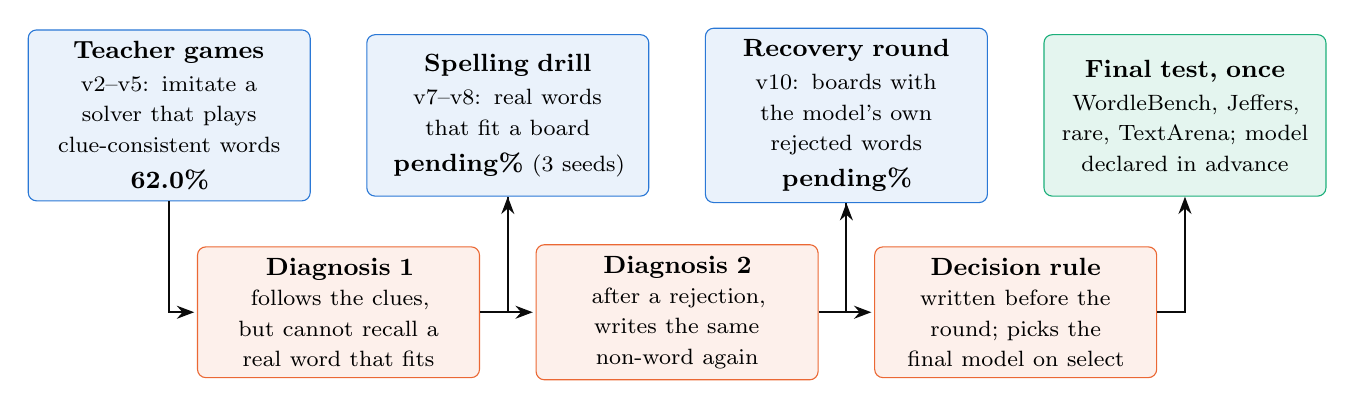
\begin{tikzpicture}[
  font=\small,
  train/.style={draw=ovblue, fill=ovblue!10, rounded corners=3pt, align=center, text width=3.3cm,
                minimum height=2.05cm, inner sep=4pt},
  diag/.style={draw=ovorange, fill=ovorange!10, rounded corners=3pt, align=center, text width=3.3cm,
               minimum height=1.5cm, inner sep=4pt},
  test/.style={draw=ovaqua, fill=ovaqua!12, rounded corners=3pt, align=center, text width=3.3cm,
               minimum height=2.05cm, inner sep=4pt},
  flow/.style={-{Stealth[length=2.2mm]}, line width=0.7pt, draw=ovink},
]
\node[train] (t1) at (0, 0)
  {\textbf{Teacher games}\\[1pt]{\footnotesize v2--v5: imitate a solver that plays clue-consistent words}\\[2pt]\textbf{62.0\%}};
\node[train] (t2) at (4.3, 0)
  {\textbf{Spelling drill}\\[1pt]{\footnotesize v7--v8: real words that fit a board}\\[2pt]\textbf{\R{agg:v8:select:alone:mean}\%} {\footnotesize(3 seeds)}};
\node[train] (t3) at (8.6, 0)
  {\textbf{Recovery round}\\[1pt]{\footnotesize v10: boards with the model's own rejected words}\\[2pt]\textbf{\W{select}{v10-s1}{}\%}};
\node[test] (t4) at (12.9, 0)
  {\textbf{Final test, once}\\[1pt]{\footnotesize WordleBench, Jeffers, rare, TextArena; model declared in advance}};
\node[diag] (d1) at (2.15, -2.5)
  {\textbf{Diagnosis 1}\\{\footnotesize follows the clues, but cannot recall a real word that fits}};
\node[diag] (d2) at (6.45, -2.5)
  {\textbf{Diagnosis 2}\\{\footnotesize after a rejection, writes the same non-word again}};
\node[diag] (d3) at (10.75, -2.5)
  {\textbf{Decision rule}\\{\footnotesize written before the round; picks the final model on select}};
\draw[flow] (t1.south) |- ([xshift=-1pt]d1.west);
\draw[flow] (d1.east) -| (t2.south);
\draw[flow] (t2.south) |- ([xshift=-1pt]d2.west);
\draw[flow] (d2.east) -| (t3.south);
\draw[flow] (t3.south) |- ([xshift=-1pt]d3.west);
\draw[flow] (d3.east) -| (t4.south);
\end{tikzpicture}
}
\caption{Method overview. Each training round (top) answers a diagnosis of the lost games of the round before it (bottom). Percentages are wins on the 534 select words for the model alone under the strict rule (v8: mean of three seeds). A rule written before the last round picks the final model on select, and the test sets are scored once at the end.}
\label{fig:overview}
\end{figure}

Our contributions are:
\begin{itemize}
\item A strict, frozen evaluation protocol. It has a selection split, a development split, test sets that we score once, three labelled rule sets, and an independent replay audit of every reported game (Section~\ref{sec:protocol}).
\item A finding about two public leaderboards. Neither checks guesses against a dictionary, so a misspelled guess still gets feedback there (Section~\ref{sec:rules}).
\item Two diagnoses of a small model's Wordle losses and one targeted fix for each: a balanced spelling drill (Sections~\ref{sec:diagnosis} and~\ref{sec:drill-results}) and a recovery round on the model's own rejected words (Sections~\ref{sec:stuck} and~\ref{sec:recovery-results}).
\item Negative results. GRPO \citep{shao2024deepseekmath}, a stronger teacher, whole-word output and self-distillation did not raise the model-alone score (Section~\ref{sec:negative}).
\item A full account of training on free Kaggle T4 GPUs, with the failures we met and the compute we used (Appendices~\ref{app:engineering} and~\ref{app:compute}).
\end{itemize}

Section~\ref{sec:related} covers related work.
Section~\ref{sec:protocol} gives the task and the protocol, and Section~\ref{sec:method} the training method.
Section~\ref{sec:results} reports the development results in the order of the rounds, and Section~\ref{sec:final} the single final test.
Sections~\ref{sec:discussion} and~\ref{sec:limitations} discuss the results and their limits.

% ============================================================================
\section{Related work}
\label{sec:related}

\paragraph{Solving Wordle.} Exact dynamic programming gives the optimal policy for the classic answer list \citep{bertsimas2022wordle}. The generalised game is NP-hard \citep{lokshtanov2022wordle,rosenbaum2022wordle}. Reinforcement learning can find strategies that a person can follow \citep{anderson2022wordle}. These solvers work on word lists directly. Our teacher is one of them: a lookahead beam search that is within 0.0004 guesses of the optimum (Section~\ref{sec:teacher}). In our setting a language model plays through text and must also write each guess.

\paragraph{Language models that play Wordle.} WordleBench \citep{wordlebench} and the Jeffers Wordle-AI-Benchmark \citep{jeffers} publish their word lists and the scores of many hosted models. SnorkelWordle \citep{snorkelwordle} publishes scores but not its words. TextArena \citep{guertler2025textarena} gives a Wordle environment for reinforcement learning of language models. Larger game suites include Wordle-like games to test chat models \citep{chalamalasetti2023clembench,wu2023smartplay}. We cite the leaderboard numbers. We did not run frontier models again.

\paragraph{Spelling in subword models.} Language models see tokens, not letters. They still learn much of the character composition of their tokens \citep{itzhak2022spelling,kaushal2022tokens}, but character-level tasks show gaps \citep{edman2024cute}. Wordle makes this gap concrete, because the model must write a real word under letter-level constraints. Our output format spaces the letters of each guess, so each letter is one token. Our first diagnosis shows that the limiting skill is the recall of real words in this format.

\paragraph{Small models.} Very small models can be fluent in a narrow domain when we train them for it \citep{eldan2023tinystories}. Recent small open models are strong general bases \citep{allal2025smollm2,gemma3}. We study how far one of them can go on one reasoning game.

\paragraph{Constrained decoding.} It is standard to limit a model's output to a grammar or a vocabulary \citep{scholak2021picard,willard2023outlines,geng2023grammar}. We compare a token-level limit with a word-level variant in which the model scores whole dictionary words.

\paragraph{Imitation and reinforcement learning.} Training on teacher games is imitation learning. A student that sees only expert states drifts after one mistake \citep{ross2011dagger}. Scheduled sampling addresses the same gap between training inputs and the model's own outputs in sequence models \citep{bengio2015scheduled}. Our recovery round applies this idea to one event, a rejected guess: the model plays, and we label the states that its own errors produce. We also try GRPO \citep{shao2024deepseekmath} and the distillation of the model's search-improved choices back into its weights \citep{anthony2017exit,hinton2015distilling}.

\paragraph{Evaluation hygiene.} If many decisions use one evaluation set, its scores become optimistic \citep{dwork2015holdout,recht2019imagenet}. We therefore keep a selection set apart from test sets that we score once, and we write each decision rule before its result exists.

% ============================================================================
\section{Task and evaluation protocol}
\label{sec:protocol}

\subsection{Game and strict rule (eval-v1, frozen)}
The game has six guesses.
The feedback for each letter is G (right letter, right place), Y (in the word, elsewhere) or X (absent), with the official rule for repeated letters.
Our feedback agrees with TextArena's engine on 10,000 test pairs.
The dictionary has 2,315 answers and 10,657 more allowed guesses, 12,972 words in total, with a fixed checksum.

The \emph{strict rule} is our headline rule.
Every model output uses a turn.
If an output has no \texttt{<guess>} tag, or if its guess is not a dictionary word, it gets no feedback and still uses the turn.
Decoding is greedy.

\paragraph{Prompt.} The model sees the rules, the board so far and the number of turns left. It answers with a short state summary and then the guess in spaced letters:
\begin{quote}\small\ttfamily
Turn 3: C R O N K -> X G G G X\\
Turns left: 3\\
$\to$ <state>fixed: \_ R O N \_ | has: - | out: C E K L M S W</state>\\
\phantom{$\to$ }<guess>F R O N D</guess>
\end{quote}
A rejected guess appears on the board as \texttt{S A T O N -> INVALID (not in word list)}.

\subsection{Word sets and test-set hygiene}
Table~\ref{tab:splits} gives the word sets.
\emph{Select} chooses checkpoints, recipes and the final model.
\emph{Heldout} is a development set that we use to check select.
We score the test sets once, for a model that we declare in advance.
No training game has a WordleBench or Jeffers word as its answer (``benchmark-clean'').

\begin{table}[htbp]
\centering\small
\caption{Word sets. Select chooses checkpoints and recipes, heldout is a development set, and the test sets are scored once for a model declared in advance.}
\label{tab:splits}
\begin{adjustbox}{max width=\linewidth}
\begin{tabular}{lrl}
\toprule
Set & Words & Use \\
\midrule
train & 1,752 & answers of the teacher games \\
select & 534 & checkpoint and recipe selection (val and heldout, minus the leaderboard words) \\
heldout & 463 & development; partly overlaps select \\
WordleBench \citep{wordlebench} & 100 & test, cited frontier scores \\
Jeffers \citep{jeffers} & 50 & test, cited frontier scores \\
rare & 500 & test, answers outside the classic list \\
TextArena Wordle-v0, adapted & 500 seeds & test; ``clean'' = the 109 games whose secret is not a training answer \\
\bottomrule
\end{tabular}\end{adjustbox}
\end{table}

\subsection{Leaderboard rules and three rule sets}
\label{sec:rules}
We read the scoring code of both public leaderboards.
WordleBench (\texttt{main.py}, commit 79436c8) scores any text inside the guess tag and has no word list.
Its yellow rule also ignores repeated letters.
Jeffers (\texttt{lib/wordle-engine.ts}, commit a79acdb) accepts any five lowercase letters.
The engine imports a dictionary check but never calls it, and it replaces malformed or repeated guesses with an unused starter word.
Thus a misspelled guess gets feedback on both leaderboards, but gets no feedback under our strict rule.
We report three rules and always label them:
\begin{description}
\item[strict] (headline) as above.
\item[retry-3] a rejected non-word does not use a turn, at most three times in a row.
\item[open-vocab] any five letters a--z get feedback and use a turn, as on both leaderboards. Malformed output still loses the turn.
\end{description}
\emph{Word-level decoding} (Section~\ref{sec:decoding}) is an inference aid, not a rule.
We score it under the strict rule and always report it next to the model alone.

\subsection{Metrics and audit}
We report the win rate with a 95\% bootstrap confidence interval \citep{efron1979bootstrap}, the mean number of guesses in won games, the share of invalid turns, and the share of guesses that contradict clues the model already has.
For two models on the same words we use the exact McNemar test on the games that only one of them wins \citep{mcnemar1947}.
An independent audit script replays every reported game from the saved outputs.
It recomputes all feedback and the win rate, and every number from our own harness passed it.
TextArena's own engine scores the TextArena games, so the audit does not cover them.

% ============================================================================
\section{Method}
\label{sec:method}

\subsection{Model and training}
We use Gemma~3 270M instruction-tuned \citep{gemma3} and train all weights.
The weights stay in fp32, and we compute in fp16 only where a startup check shows that fp16 and fp32 agree.
The optimiser is AdamW with a learning rate of $5\times10^{-5}$, 100 warm-up steps, 64 samples per step, one epoch and at most 512 tokens per sample.
We keep the checkpoint with the best select win rate, which we evaluate every 500 steps.
Each session runs on Kaggle's free tier, which gives two T4 GPUs and a weekly quota of about 30 GPU hours.
Appendix~\ref{app:hparams} gives all settings.

\subsection{Teacher and teacher games}
\label{sec:teacher}
The teacher is a lookahead beam search over the full vocabulary.
With the opener SALET it needs 3.4216 guesses on average and wins all 2,315 classic games; the proven optimum is 3.4212 \citep{bertsimas2022wordle}.
TextArena rejects SALET and more than a third of the dictionary (it accepts 8,019 of the 12,972 words).
The training games therefore use a shared vocabulary of 8,035 words and the opener CRATE (3.4281 guesses, no losses).
From round v5 on, the teacher guesses only words that fit every clue.
We call it the \emph{consistent teacher}.
A small student can imitate it, but the optimal teacher often plays probe words that break the clues.
The training games include off-script states: random openings, 10\% noise moves and some invalid turns.
These states teach the student to continue after a mistake \citep{ross2011dagger}.
We also add games on 1,610 common words that are not test answers, because a model trained only on the 1,752 training answers memorised them (Section~\ref{sec:memorise}).

\subsection{Spelling drill}
\label{sec:drill}
A drill sample is a board and one real common word that fits it, in the same prompt format.
We build boards only around training-side hidden words, never around a development or test answer.
Every common word is a target the same number of times.
The common words are the 5,557 words with a wordfreq Zipf value of 2.0 or more \citep{speer2022wordfreq}.
Half of the earlier teacher games are replayed in the same data.

\emph{Disclosure.} A target can be any common public word.
So 527 of the 534 select words and 147 of the 148 leaderboard words are spelling targets on boards built around other words.
A strict variant (v7s) never uses a development or test word as a target, and we report it next to the main variant.

Round v7 uses 30 samples per word and boards of 1--4 guesses.
Round v8 uses 40 samples per word, boards of 1--5 guesses and up to two rejected non-words per board, because v7's invalid turns were mostly in turns 4--6.

\subsection{Recovery round}
\label{sec:recovery}
The drill boards contain rejected words, but these are random near-misses of a target.
They are never the word that the model itself would write next.
The recovery round uses the model's own errors instead, in the manner of DAgger \citep{ross2011dagger}:
\begin{enumerate}
\item The model plays alone on training-side hidden words. These are the 8,546 valid words that are neither a development or test answer nor an answer of its training games. Each GPU takes one half.
\item At each turn where the game first rejects one of the model's own non-words and a turn is left, we make up to four training samples. Each sample is the game as played, with the rejected word on the board, and its target is a real word that fits the clues and was not played. One target is the hidden word. With probability 0.3 the board also shows the rejection twice, as when the model repeats it.
\item We train the model on these samples together with 4\% of the v8 data as replay, for two epochs, with a learning rate of $2\times10^{-5}$ and 30 warm-up steps. We evaluate select every 100 steps.
\end{enumerate}
A data generator raises an error if a game's answer is a development or test word.

\subsection{Word-level decoding}
\label{sec:decoding}
A token-level dictionary limit commits to the most likely allowed first letters.
Then it must complete whatever word starts with them.
Word-level decoding runs a beam search (width 16) over a trie of the 12,972 dictionary words in the spaced-letter format.
It returns the word with the highest summed log-probability under the model, and it excludes words already played.
The code never uses the clues, so the model alone decides which real word fits.

\subsection{Training rounds and decision rules}
\label{sec:rounds}
Table~\ref{tab:rounds} lists the training rounds.
Before each round, we wrote into the project roadmap what the round tests and what we would do for each possible result.
Appendix~\ref{app:prereg} gives the rules that chose the final model.
No test-set number chose any training step.

\begin{table}[htbp]
\centering\small
\caption{Training rounds. Each round answers one question raised by the round before it.}
\label{tab:rounds}
\begin{adjustbox}{max width=\linewidth}
\begin{tabular}{llll}
\toprule
Round & Starting weights & New training data & Question \\
\midrule
v2 & pretrained model & optimal-teacher games on the 1,752 training answers & Does imitation work at all? \\
v3, v3c & pretrained model & + games on 1,610 extra common answers (v3c: benchmark-clean) & Does the model memorise? \\
v5 & pretrained model & consistent-teacher games & Does a clue-consistent teacher help? \\
v6, v6w & pretrained model & stronger teacher; whole-word output (v6w) & Strategy or output format? \\
v7, v7s & v5 s1 & spelling drill, 30 per word (v7s: strict targets) & Is spelling the limit? \\
v8 & v7 s1 & deep drill, 40 per word, boards of 1--5 guesses & Late-turn spelling \\
v9 & v8 s2 & one more v8 round on fresh boards & Has the drill saturated? \\
v10 & v8 s3 & recovery samples from the model's own rejected words & Can it recover from a rejection? \\
\bottomrule
\end{tabular}\end{adjustbox}
\end{table}

% ============================================================================
\section{Results on the development sets}
\label{sec:results}

We report the results in the order of the rounds, because each diagnosis chose the next round.
Table~\ref{tab:dev} collects the main development results and Figure~\ref{fig:rounds} plots them.

\begin{table}[htbp]
\centering\small
\caption{Development results, win rate in \% (select: 534 games; heldout: 463 games). All rows passed the audit. Bold: the final model. The select score alone for v5 s1 is its training-time evaluation.}
\label{tab:dev}
\setlength{\tabcolsep}{4pt}
\begin{adjustbox}{max width=\linewidth}
\begin{tabular}{lcccccc}
\toprule
 & \multicolumn{4}{c}{select} & \multicolumn{2}{c}{heldout} \\
\cmidrule(lr){2-5}\cmidrule(lr){6-7}
Model & strict & retry-3 & open-vocab & word-level & strict & word-level \\
\midrule
SFT v5 s1 & 62.0 & \W{select}{v5-s1}{-retry3} & \W{select}{v5-s1}{-open} & \W{select}{v5-s1}{\WB} & \W{heldout}{v5-s1}{} & \W{heldout}{v5-s1}{\WB} \\
SFT v6 s1 (stronger teacher) & \W{select}{v6-s1}{} & -- & -- & \W{select}{v6-s1}{\WB} & \W{heldout}{v6-s1}{} & \W{heldout}{v6-s1}{\WB} \\
v7 s1 (drill) & \W{select}{v7-s1}{} & \W{select}{v7-s1}{-retry3} & \W{select}{v7-s1}{-open} & \W{select}{v7-s1}{\WB} & \W{heldout}{v7-s1}{} & \W{heldout}{v7-s1}{\WB} \\
v7s s1 (strict drill) & \W{select}{v7s-s1}{} & \W{select}{v7s-s1}{-retry3} & \W{select}{v7s-s1}{-open} & -- & \W{heldout}{v7s-s1}{} & -- \\
v8 s1 (deep drill) & \W{select}{v8-s1}{} & \W{select}{v8-s1}{-retry3} & \W{select}{v8-s1}{-open} & \W{select}{v8-s1}{\WB} & \W{heldout}{v8-s1}{} & \W{heldout}{v8-s1}{\WB} \\
v8 s2 & \W{select}{v8-s2}{} & \W{select}{v8-s2}{-retry3} & \W{select}{v8-s2}{-open} & \W{select}{v8-s2}{\WB} & \W{heldout}{v8-s2}{} & \W{heldout}{v8-s2}{\WB} \\
v8 s3 (base of v10) & \W{select}{v8-s3}{} & \W{select}{v8-s3}{-retry3} & \W{select}{v8-s3}{-open} & \W{select}{v8-s3}{\WB} & \W{heldout}{v8-s3}{} & \W{heldout}{v8-s3}{\WB} \\
v8 mean ($k$ = \R{agg:v8:select:alone:k}) & \R{agg:v8:select:alone:mean}\,$\pm$\,\R{agg:v8:select:alone:sd} & \R{agg:v8:select:retry:mean} & \R{agg:v8:select:open:mean} & \R{agg:v8:select:word:mean}\,$\pm$\,\R{agg:v8:select:word:sd} & \R{agg:v8:heldout:alone:mean} & \R{agg:v8:heldout:word:mean} \\
v9 s1 (one more round from v8 s2) & \W{select}{v9-s1}{} & \W{select}{v9-s1}{-retry3} & \W{select}{v9-s1}{-open} & \W{select}{v9-s1}{\WB} & \W{heldout}{v9-s1}{} & \W{heldout}{v9-s1}{\WB} \\
\midrule
\textbf{v10 s1} (recovery round) & \textbf{\W{select}{v10-s1}{}} & \W{select}{v10-s1}{-retry3} & \W{select}{v10-s1}{-open} & \textbf{\W{select}{v10-s1}{\WB}} & \textbf{\W{heldout}{v10-s1}{}} & \W{heldout}{v10-s1}{\WB} \\
v10 s2 & \W{select}{v10-s2}{} & \W{select}{v10-s2}{-retry3} & \W{select}{v10-s2}{-open} & \W{select}{v10-s2}{\WB} & \W{heldout}{v10-s2}{} & \W{heldout}{v10-s2}{\WB} \\
v10 mean ($k$ = \R{agg:v10:select:alone:k}) & \R{agg:v10:select:alone:mean}\,$\pm$\,\R{agg:v10:select:alone:sd} & \R{agg:v10:select:retry:mean} & \R{agg:v10:select:open:mean} & \R{agg:v10:select:word:mean}\,$\pm$\,\R{agg:v10:select:word:sd} & \R{agg:v10:heldout:alone:mean} & \R{agg:v10:heldout:word:mean} \\
\bottomrule
\end{tabular}\end{adjustbox}
\end{table}

\begin{figure}[htbp]
\centering
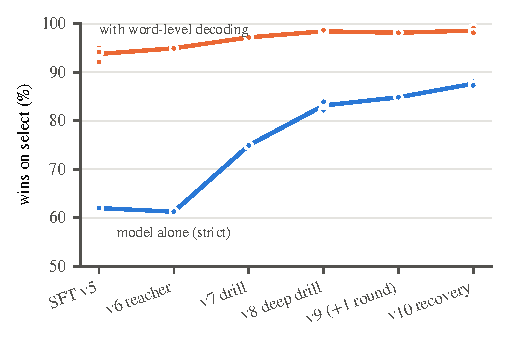
\includegraphics[width=0.48\linewidth]{figures/rounds.pdf}\hfill
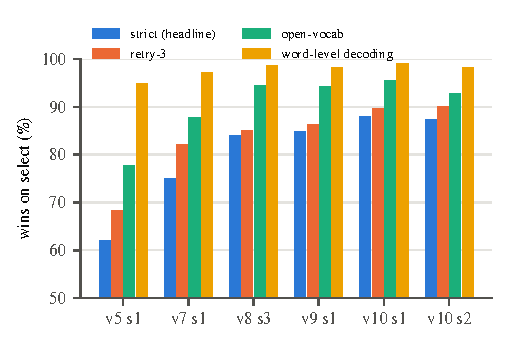
\includegraphics[width=0.48\linewidth]{figures/rules.pdf}
\caption{Left: select win rate by training round, one dot per seed, with a line through the seed means. Right: the same models under the three rule sets and with word-level decoding.}
\label{fig:rounds}
\end{figure}

\subsection{From memorising to following the clues}
\label{sec:memorise}
We first trained only on teacher games for the 1,752 training answers (v2).
The model won 20 of 20 games on training answers, 13 of 20 on unseen answers, and \W{heldout}{v2}{}\% of heldout games.
Every invalid turn on unseen answers was an invented word.
Games on 1,610 extra common answers (v3) raised heldout to \W{heldout}{v3}{}\%.
With the optimal teacher, however, 49\% of the model's guesses contradicted clues that it already had.
The consistent teacher (v5) cut this share to 7.5\%.
It also raised heldout alone from \W{heldout}{v3c}{}\% (benchmark-clean v3) to \W{heldout}{v5-s1}{}\%.

\subsection{Teacher and output limits}
Table~\ref{tab:ablation} separates the effect of the teacher from the effect of an output limit.
Word-level decoding adds 32--36 points over the model alone and 17--24 points over a token-level limit.
No training change in this study had an effect of this size.
The consistent teacher does not raise wins under word-level decoding.
But it cuts clue contradictions from 44\% to 9\% and saves about 0.2 guesses per win.
On a T4 GPU and on a laptop CPU, the word-level results were the same game for game.

\begin{table}[htbp]
\centering\small
\caption{Heldout (463 games), strict rule. Word-level decoding causes most of the wins; the consistent teacher makes play shorter and consistent with the clues.}
\label{tab:ablation}
\begin{tabular}{lcc}
\toprule
 & v3c (optimal teacher) & v5 s1 (consistent teacher) \\
\midrule
model alone & \W{heldout}{v3c}{}\% & \W{heldout}{v5-s1}{}\% \\
token-level limit & \W{heldout}{v3c}{-constrained-wordle}\% & \W{heldout}{v5-s1}{-constrained-wordle}\% \\
word-level decoding & \W{heldout}{v3c}{\WB}\% & \W{heldout}{v5-s1}{\WB}\% \\
guesses per win, word-level & \R{heldout:hf-sft-gemma270m-v3c-best\WB:gw} & \R{heldout:hf-sft-gemma270m-v5-s1-best\WB:gw} \\
guesses that contradict known clues, word-level & \R{heldout:hf-sft-gemma270m-v3c-best\WB:contra}\% & \R{heldout:hf-sft-gemma270m-v5-s1-best\WB:contra}\% \\
\bottomrule
\end{tabular}
\end{table}

\subsection{First diagnosis: the model alone fails at spelling}
\label{sec:diagnosis}
We read the select games of SFT v6 (model alone).
Of the 272 games with no invalid turn, the model won 269.
All invalid turns were well-formed five-letter non-words.
Of these, 78\% fit every clue and 38\% were one letter from the answer.
97.6\% of the model's valid guesses were words that it had seen as training targets, and these covered only 6,871 of the 12,972 dictionary words.
The win rate rose with the number of times the answer had been a training target: 12.5\% (never), 43.6\% (1--9 times), 72.4\% (10--99) and 77.1\% (100 or more).
The model knows the pattern that the answer must match, but it cannot recall a real word with that pattern.
This diagnosis led to the spelling drill (Section~\ref{sec:drill}).

\subsection{Effect of the spelling drill}
\label{sec:drill-results}
The drill raised the model-alone score on select from 62.0\% to \W{select}{v7-s1}{}\% (v7) and \R{agg:v8:select:alone:mean}\% (v8, mean of three seeds).
Heldout moved by a similar amount.
Word-level decoding rose to \R{agg:v8:select:word:mean}\%.
The three v8 seeds lie within \R{agg:v8:select:alone:sd} points (standard deviation) of each other.

On the same 534 select words, v8 s1 wins \Pp{v7-s1}{v8-s1}{bonly} games that v7 s1 loses, and loses \Pp{v7-s1}{v8-s1}{aonly} games that v7 s1 wins ($p$ \Pp{v7-s1}{v8-s1}{p}).
For v8 s2 the counts are \Pp{v7-s1}{v8-s2}{bonly} and \Pp{v7-s1}{v8-s2}{aonly} ($p$ \Pp{v7-s1}{v8-s2}{p}).
A second round of the same drill (v9) gave little.
Against v8 s3 it won \Pp{v8-s3}{v9-s1}{bonly} more games and lost \Pp{v8-s3}{v9-s1}{aonly} ($p$ = \Pp{v8-s3}{v9-s1}{p}), and its word-level score was lower.

The strict drill (v7s) scored below its starting model.
When the drill never shows a word, the model spells that word worse than before.
Two readings fit this result.
Spelling may be learned word by word.
Or v7s may have learned that about 800 words, which are exactly the likely answers, are never the right output.
These data cannot separate the two readings, and every drill-based number in this paper depends on the disclosed choice of targets.

\paragraph{Training curves.} Figure~\ref{fig:curves} (left) shows the select score during training. Each drill round starts below its starting model (v8: 57--63\% at step 500, from 74.9\%) and passes it only after about 3,000 steps. Neither v8 seed shows a clear plateau at the end of its single epoch. The recovery round is different. It starts at the level of its base and peaks early (v10 s1 at step 300 of 688).

\begin{figure}[htbp]
\centering
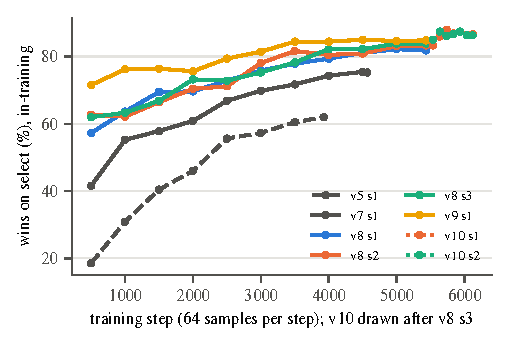
\includegraphics[width=0.48\linewidth]{figures/curves.pdf}\hfill
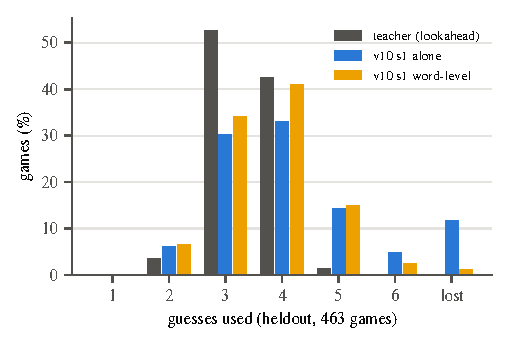
\includegraphics[width=0.48\linewidth]{figures/histogram.pdf}
\caption{Left: select win rate during training (greedy, model alone). The v10 curves start from the last step of v8 s3. Right: guesses used on heldout by the teacher and by the final model, alone and with word-level decoding.}
\label{fig:curves}
\end{figure}

\subsection{Second diagnosis: stuck on a rejected word}
\label{sec:stuck}
After the drill, \G{v8-s1}{lostwithinvalid} of the \G{v8-s1}{lost} select games that v8 s1 lost contain an invalid turn.
\G{v8-s1}{fit}\% of its non-words fit the clues and \G{v8-s1}{near}\% are one letter from the answer.
Invalid turns are rare in turns 1--3 and become frequent after turn 3 (Figure~\ref{fig:turns}).
Clue contradictions fell to 2--3\%.

The invalid turns are not independent errors.
Table~\ref{tab:stuck} separates the first non-word in a game from exact repeats of a word that the game has already rejected.
v8 s1 writes a non-word in only \G{v8-s1}{gameswithnonword} of 534 games, and it loses all of them.
After a first non-word, its next turn is the same word in \G{v8-s1}{nextsame} cases and a valid word in \G{v8-s1}{nextvalid} (Figure~\ref{fig:examples}b).
The prompt shows the rejection, but the model's state summary does not change, so it writes the same guess.
The base of v10 (v8 s3) behaves in the same way: \G{v8-s3}{nextsame} repeats against \G{v8-s3}{nextvalid} valid words.

This pattern explains two earlier numbers.
Retry-3 adds only about 2 points, because the model spends its retries on the same word.
Under open-vocab the same non-word gets feedback, the board changes, and the model continues.
That is why v8 scores about 11 points higher under open-vocab than under the strict rule (mean of three seeds).
The model had never trained on a board on which its own first choice had just been rejected.
This is the covariate shift of imitation learning \citep{ross2011dagger}, here for one specific event.
This diagnosis led to the recovery round (Section~\ref{sec:recovery}).

\begin{figure}[htbp]
\centering
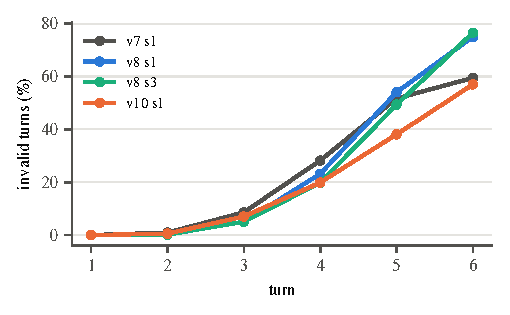
\includegraphics[width=0.48\linewidth]{figures/invalid_by_turn.pdf}\hfill
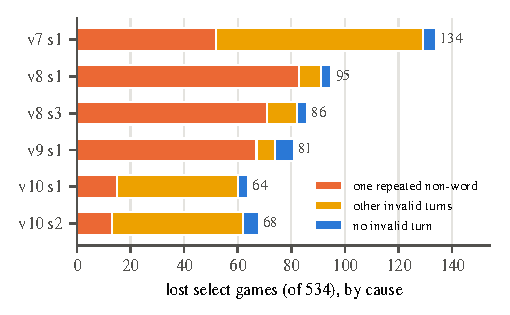
\includegraphics[width=0.48\linewidth]{figures/losses.pdf}
\caption{Left: share of invalid turns by turn number, among games still running. Late turns are harder, and fewer games reach them. Right: lost games by cause. Before the recovery round, most losses are one non-word written again and again; after it, few are. Both panels: select, model alone, strict rule.}
\label{fig:turns}
\end{figure}

\begin{table}[htbp]
\centering\small
\caption{Rejected words on select (534 games, model alone, strict rule). After the drill (v8) the model seldom writes a non-word, but then it repeats it. After the recovery round (v10) it writes a different, valid word in most cases.}
\label{tab:stuck}
\begin{adjustbox}{max width=\linewidth}
\begin{tabular}{lccccc}
\toprule
 & v7 s1 & v8 s1 & v8 s3 & v10 s1 & v10 s2 \\
\midrule
games with a non-word & \G{v7-s1}{gameswithnonword} & \G{v8-s1}{gameswithnonword} & \G{v8-s3}{gameswithnonword} & \G{v10-s1}{gameswithnonword} & \G{v10-s2}{gameswithnonword} \\
first non-words in a game & \G{v7-s1}{firsttime} & \G{v8-s1}{firsttime} & \G{v8-s3}{firsttime} & \G{v10-s1}{firsttime} & \G{v10-s2}{firsttime} \\
exact repeats of a rejected word & \G{v7-s1}{repeats} & \G{v8-s1}{repeats} & \G{v8-s3}{repeats} & \G{v10-s1}{repeats} & \G{v10-s2}{repeats} \\
next turn after a first non-word: a valid word & \G{v7-s1}{nextvalid} & \G{v8-s1}{nextvalid} & \G{v8-s3}{nextvalid} & \G{v10-s1}{nextvalid} & \G{v10-s2}{nextvalid} \\
next turn after a first non-word: the same word & \G{v7-s1}{nextsame} & \G{v8-s1}{nextsame} & \G{v8-s3}{nextsame} & \G{v10-s1}{nextsame} & \G{v10-s2}{nextsame} \\
lost games & \G{v7-s1}{lost} & \G{v8-s1}{lost} & \G{v8-s3}{lost} & \G{v10-s1}{lost} & \G{v10-s2}{lost} \\
lost games whose invalid turns are one repeated word & \G{v7-s1}{lostononerepeated} & \G{v8-s1}{lostononerepeated} & \G{v8-s3}{lostononerepeated} & \G{v10-s1}{lostononerepeated} & \G{v10-s2}{lostononerepeated} \\
games won, by invalid turns in the game: none & \G{v7-s1}{inv0} & \G{v8-s1}{inv0} & \G{v8-s3}{inv0} & \G{v10-s1}{inv0} & \G{v10-s2}{inv0} \\
\quad one & \G{v7-s1}{inv1} & \G{v8-s1}{inv1} & \G{v8-s3}{inv1} & \G{v10-s1}{inv1} & \G{v10-s2}{inv1} \\
\quad two & \G{v7-s1}{inv2} & \G{v8-s1}{inv2} & \G{v8-s3}{inv2} & \G{v10-s1}{inv2} & \G{v10-s2}{inv2} \\
\quad three or more & \G{v7-s1}{inv3} & \G{v8-s1}{inv3} & \G{v8-s3}{inv3} & \G{v10-s1}{inv3} & \G{v10-s2}{inv3} \\
\bottomrule
\end{tabular}\end{adjustbox}
\end{table}

\begin{figure}[htbp]
\centering\small
\begin{tabular}[t]{@{}r@{\;\,}l@{}}
\multicolumn{2}{@{}l}{\textbf{(a) A win}: answer \textsc{abbey}} \\[2pt]
1 & \tx{C}\tx{R}\ty{A}\tx{T}\ty{E}\;{\scriptsize\ttfamily XXYXY} \\
2 & \tx{D}\ty{A}\tx{L}\tg{E}\tx{S}\;{\scriptsize\ttfamily XYXGX} \\
3 & \tg{A}\tx{P}\tx{N}\tg{E}\tx{A}\;{\scriptsize\ttfamily GXXGX} \\
4 & \tg{A}\tg{B}\tg{B}\tg{E}\tg{Y}\;{\scriptsize\ttfamily GGGGG} \\
\end{tabular}
\hfill
\begin{tabular}[t]{@{}r@{\;\,}l@{}}
\multicolumn{2}{@{}l}{\textbf{(b) Stuck on a rejected word}: answer \textsc{baton}} \\[2pt]
1 & \tx{C}\tx{R}\ty{A}\ty{T}\tx{E}\;{\scriptsize\ttfamily XXYYX} \\
2 & \ty{T}\tg{A}\tx{L}\tg{O}\tg{N}\;{\scriptsize\ttfamily YGXGG} \\
3 & \tn{S}\tn{A}\tn{T}\tn{O}\tn{N}\;{\scriptsize\ttfamily rejected} \\
4 & \tn{S}\tn{A}\tn{T}\tn{O}\tn{N}\;{\scriptsize\ttfamily rejected} \\
5 & \tn{S}\tn{A}\tn{T}\tn{O}\tn{N}\;{\scriptsize\ttfamily rejected} \\
6 & \tn{S}\tn{A}\tn{T}\tn{O}\tn{N}\;{\scriptsize\ttfamily rejected} \\
\end{tabular}
\\[8pt]
\begin{tabular}[t]{@{}r@{\;\,}l@{}}
\multicolumn{2}{@{}l}{\textbf{(c) A trap, word-level decoding}: answer \textsc{swell}} \\[2pt]
1 & \tx{C}\tx{R}\tx{A}\tx{T}\ty{E}\;{\scriptsize\ttfamily XXXXY} \\
2 & \tx{D}\ty{E}\ty{L}\tx{E}\ty{S}\;{\scriptsize\ttfamily XYYXY} \\
3 & \tg{S}\tx{K}\tg{E}\tg{L}\tg{L}\;{\scriptsize\ttfamily GXGGG} \\
4 & \tg{S}\tx{H}\tg{E}\tg{L}\tg{L}\;{\scriptsize\ttfamily GXGGG} \\
5 & \tg{S}\tx{M}\tg{E}\tg{L}\tg{L}\;{\scriptsize\ttfamily GXGGG} \\
6 & \tg{S}\tx{P}\tg{E}\tg{L}\tg{L}\;{\scriptsize\ttfamily GXGGG} \\
\end{tabular}
\hfill
\begin{tabular}[t]{@{}r@{\;\,}l@{}}
\multicolumn{2}{@{}l}{\textbf{(d) Recovery after a rejection, v10 s1}: answer \textsc{badly}} \\[2pt]
1 & \tx{C}\tx{R}\ty{A}\tx{T}\tx{E}\;{\scriptsize\ttfamily XXYXX} \\
2 & \tx{S}\tg{A}\ty{L}\tx{O}\tx{N}\;{\scriptsize\ttfamily XGYXX} \\
3 & \tx{G}\tg{A}\tx{I}\tg{L}\tg{Y}\;{\scriptsize\ttfamily XGXGG} \\
4 & \tx{M}\tg{A}\tg{D}\tg{L}\tg{Y}\;{\scriptsize\ttfamily XGGGG} \\
5 & \tn{P}\tn{A}\tn{D}\tn{L}\tn{Y}\;{\scriptsize\ttfamily rejected} \\
6 & \tg{B}\tg{A}\tg{D}\tg{L}\tg{Y}\;{\scriptsize\ttfamily GGGGG} \\
\end{tabular}

\caption{Four select games. The letters after each guess give the feedback: G right place, Y elsewhere in the word, X absent. A boxed guess was rejected as a non-word and used the turn. (a)--(c) are games of v8 s1. In (b) the prompt shows that \textsc{saton} was rejected, yet the model writes it again. In (c), with word-level decoding, every guess is a real word, and the loss comes from a set of words that differ in one letter. (d) After the recovery round, the model follows a rejected word with a different, real word.}
\label{fig:examples}
\end{figure}

\subsection{Effect of the recovery round}
\label{sec:recovery-results}
Per GPU, the base played 4,273 training-side words alone and won 1,340 and 1,403 of them.
These words are rarer than the answer lists, so the base loses most of them.
The games gave 2,261 and 2,162 first rejections, and from them 3,077 and 2,879 recovery samples.
With the replay data, each seed trained on about 22,000 samples for 688 steps, which took 30 minutes on one T4.

Alone, the two seeds gained 3.4 and 4.1 points on select and 2.6 and 3.6 points on heldout (Table~\ref{tab:dev}).
The final model, v10 s1, wins \W{select}{v10-s1}{}\% of select games alone (95\% CI \R{select:hf-sft-gemma270m-v10-s1-best:lo}--\R{select:hf-sft-gemma270m-v10-s1-best:hi}), against \W{select}{v8-s3}{}\% for its base.
On the same words it wins \Pp{v8-s3}{v10-s1}{bonly} games that the base loses and loses \Pp{v8-s3}{v10-s1}{aonly} that the base wins ($p$ = \Pp{v8-s3}{v10-s1}{p}).
For v10 s2 the counts are \Pp{v8-s3}{v10-s2}{bonly} and \Pp{v8-s3}{v10-s2}{aonly} ($p$ = \Pp{v8-s3}{v10-s2}{p}).
The two v10 seeds do not differ significantly (\Pp{v10-s1}{v10-s2}{bonly} against \Pp{v10-s1}{v10-s2}{aonly} games, $p$ = \Pp{v10-s1}{v10-s2}{p}).
Select chose the checkpoint, so the select score is optimistic.
Heldout did not choose anything in this round, and it shows the same gain (\W{heldout}{v8-s3}{}\% to \W{heldout}{v10-s1}{}\%).
Word-level decoding stays at \W{select}{v10-s1}{\WB}\% for v10 s1.

Table~\ref{tab:stuck} shows where the gain comes from.
After a first non-word, v10 s1 writes a valid word in \G{v10-s1}{nextvalid} cases and the same word in \G{v10-s1}{nextsame}.
Games with exactly one invalid turn are now won \G{v10-s1}{inv1} times, against \G{v8-s3}{inv1} for the base.
Losses that consist of one repeated non-word fell from \G{v8-s3}{lostononerepeated} to \G{v10-s1}{lostononerepeated}.
The gap between open-vocab and the strict rule fell from 10.5 points for the base to 7.5 points (\W{select}{v10-s1}{-open}\% against \W{select}{v10-s1}{}\%).
This agrees with the diagnosis, because open-vocab hides exactly this failure.

Two problems remain.
First, the model writes a first non-word more often than its base (\G{v10-s1}{gameswithnonword} games against \G{v8-s3}{gameswithnonword}).
We do not know the cause.
One possibility is that the recovery data shows non-words that are followed by a fix, so writing one costs less in training.
Second, the model still wins \G{v10-s1}{inv3} games with three or more invalid turns.
In most of these lost games the model no longer repeats one word; it writes several different non-words (Figure~\ref{fig:turns}, right).
So the model now tries again, but its next attempts are often non-words too.
The remaining gap is again spelling, now under pressure late in the game.

\subsection{What did not help}
\label{sec:negative}
\paragraph{GRPO.} From SFT v3, GRPO lowered the share of invalid turns (23.3\% to 19.4\% on heldout) and raised the score on TextArena's clean subset. Heldout wins did not rise (\W{heldout}{v3}{}\% to \R{heldout:hf-grpo-gemma270m-v3-best:win}\%). From SFT v5, none of six GRPO checkpoints beat step 0 on select (62.0\% to 60.1--60.5\%). A probable cause is that the rollouts used mostly memorised answers, so a quarter of the groups had no reward signal. We did not run GRPO on the drilled models.

\paragraph{A stronger teacher.} In v6 the teacher preferred common words on ties and played probe words on trap sets. The model scored \W{select}{v6-s1}{}\% alone on select, no better than v5, and it used more guesses per win.

\paragraph{Whole-word output.} In v6w the model wrote each guess as one word instead of spaced letters. Invalid turns fell to about 5\%, but half of the guesses contradicted the clues, and wins fell to \W{select}{v6w-s1}{}\%.

\paragraph{Self-distillation.} Training on the model's own word-level wins (v5-d1) added 3.0 points alone. But word-level decoding fell from \W{select}{v5-s1}{\WB}\% to \W{select}{v5-d1}{\WB}\%, below our pre-set floor.

% ============================================================================
\section{Final test}
\label{sec:final}
A rule written before the last training round chose the final model on select (Appendix~\ref{app:prereg}).
We declared it before we scored any test set for it: \FINALNAME.
Table~\ref{tab:final} gives its only scores on the test sets.

\begin{table}[htbp]
\centering\small
\caption{Final test, win rate in \% (95\% CI). We scored each set once for the declared final model. Others made the cited scores on the same word sets, under the leaderboard rules of Section~\ref{sec:rules} (no dictionary), with other prompts and settings.}
\label{tab:final}
\setlength{\tabcolsep}{3.5pt}
\begin{adjustbox}{max width=\linewidth}
\begin{tabular}{lccccl}
\toprule
 & \multicolumn{3}{c}{model alone} & word-level & cited best \\
\cmidrule(lr){2-4}
Set & strict & retry-3 & open-vocab & decoding & (no dictionary) \\
\midrule
WordleBench (100) & \FC{wordlebench}{} & \F{wordlebench}{-retry3} & \FC{wordlebench}{-open} & \FC{wordlebench}{\WB} & GPT-5: 99 (3.59 guesses) \\
Jeffers (50) & \FC{jeffers}{} & \F{jeffers}{-retry3} & \FC{jeffers}{-open} & \FC{jeffers}{\WB} & GPT-5: 100 (3.58) \\
rare (500) & \FC{rare}{} & \F{rare}{-retry3} & \FC{rare}{-open} & \FC{rare}{\WB} & -- \\
TextArena, all (500) & \FP{}{all} & -- & -- & \FP{-constrained-shared-word}{all} & -- \\
TextArena, clean (109) & \FP{}{clean} & -- & -- & \FP{-constrained-shared-word}{clean} & -- \\
\bottomrule
\end{tabular}\end{adjustbox}
\end{table}

\paragraph{Comparison with the cited scores.} With word-level decoding the model wins \F{wordlebench}{\WB}\% of WordleBench games and \F{jeffers}{\WB}\% of Jeffers games, 2 and 4 points below the cited GPT-5 scores. The leaderboards use no dictionary, so their rule is open-vocab, and under that rule the model alone wins \F{wordlebench}{-open}\% and \F{jeffers}{-open}\%. On WordleBench this is in the range of many frontier models (94--98\% \citep{wordlebench}), with the caveats of Section~\ref{sec:limitations}. Under the strict rule the model alone wins \F{wordlebench}{}\% and \F{jeffers}{}\%.

\paragraph{Agreement with the development sets.} WordleBench agrees with select (\F{wordlebench}{}\% against \W{select}{v10-s1}{}\% alone). Jeffers is lower alone (\F{jeffers}{}\%), but it has only 50 games and its interval reaches \R{jeffers:hf-sft-gemma270m-\FINALRUN-best:hi}\%. With word-level decoding the two sets are 2.1 and 3.1 points below select (\W{select}{v10-s1}{\WB}\%). The rare set is the hardest: its answers are outside the classic answer list, and the model wins \F{rare}{}\% alone and \F{rare}{\WB}\% with word-level decoding, with about 4.6 guesses per win. The model's word knowledge is concentrated on common words.

\paragraph{The lost games.} Appendix~\ref{app:games} shows every WordleBench game that the final model lost. Alone, it lost 13. Ten of them contain non-words, and in nine a rejected word is written again, so the failure of Section~\ref{sec:stuck} is reduced but still present on test words. The other three are trap sets of real words that differ in one letter (\textsc{bonus}, \textsc{laser}, \textsc{water}), and these are exactly the three games that word-level decoding loses.

\paragraph{Progress since the earlier final model.} On the same two sets, the earlier declared final model (SFT v5 s1) won 95.0\% and 86.0\% with word-level decoding and 60.0\% and 54.0\% alone. The spelling drill and the recovery round raise the model-alone scores by 27 and 20 points.

\paragraph{Guesses per win.} On WordleBench the final model needs \R{wordlebench:hf-sft-gemma270m-\FINALRUN-best\WB:gw} guesses per win with word-level decoding and \R{wordlebench:hf-sft-gemma270m-\FINALRUN-best:gw} alone. On Jeffers it needs \R{jeffers:hf-sft-gemma270m-\FINALRUN-best\WB:gw} and \R{jeffers:hf-sft-gemma270m-\FINALRUN-best:gw}. The cited values for GPT-5 are 3.59 and 3.58.

\paragraph{Earlier test-set use.} We scored WordleBench and Jeffers twice before. The first use was for an older benchmark-clean model (v3c). The second was for SFT v5 s1, the declared final model of an earlier phase. These results did not choose any later recipe, and every later choice used select. We report the earlier uses because they still carry some risk of adaptive overfitting.

% ============================================================================
\section{Discussion}
\label{sec:discussion}

\paragraph{Three skills, found in sequence.} The losses of this model came from three skills, and each one became visible only after we fixed the one before it. The first was to follow the clues instead of a memorised answer. The second was to recall a real word that fits a pattern. The third was to recover when the game rejects a word. Aggregate scores did not show the second and third skills. We found them by reading lost games and by counting simple events, such as the turn after a first non-word. Each fix was a small data change, not a new algorithm.

\paragraph{Imitation needs the student's own states.} The drill already contained rejected words. It did not help with recovery, because those rejections were not the model's own. Training on states that the model's own errors produce did help, after one round and with fewer than 3,100 new samples. This is the DAgger argument \citep{ross2011dagger} in a small and measurable form.

\paragraph{The rule changes the comparison.} Under open-vocab the v8 models scored about 11 points higher than under the strict rule. Most of this gap came from one failure that open-vocab hides. A leaderboard that accepts any five letters therefore measures a different skill from a game that rejects non-words. We think that game papers should state this rule, and that leaderboards should report it.

\paragraph{Decoding aid against model alone.} Word-level decoding still adds about 11 points to the final model. With it, the model needs no dictionary knowledge in its weights, only the ability to rank real words. We report both numbers everywhere, because they answer different questions.

% ============================================================================
\section{Limitations}
\label{sec:limitations}
\begin{itemize}
\item \textbf{Other conditions than the leaderboards.} Other harnesses made the cited scores, with other prompts and sampling settings. Open-vocab matches their dictionary rule but stays stricter on malformed output. WordleBench's yellow rule is simpler than the rule of real Wordle. The comparison uses the same word sets, not the same conditions.
\item \textbf{Generalist against specialist.} Frontier models play zero-shot as general models. Our model is trained for one game.
\item \textbf{Spelling targets.} The drill's targets include test answers as common English words (Section~\ref{sec:drill}). The model never sees a board built around a test answer, and no training game has a test answer as its answer. The strict variant shows that this choice matters.
\item \textbf{Reuse of the selection set.} Select chose checkpoints, recipes and the final model over several rounds, so the select and heldout scores are optimistic. Only the final test is free of these choices.
\item \textbf{Seeds.} The drill recipe has three seeds and the recovery round two. Most earlier ablations have one seed, and their smaller differences (2--3 points) are within seed noise (v5: $\pm$1.5 points across seeds with word-level decoding).
\item \textbf{Efficiency.} Even with word-level decoding the model needs about 3.7 guesses per win, against 3.42 for the teacher. It seldom plays probe words that collect information.
\end{itemize}

% ============================================================================
\section{Conclusion}
\label{sec:conclusion}
A 270M-parameter model, trained on free GPUs, follows Wordle's clues almost without error.
Its losses came from spelling and then from recovery, not from strategy.
A balanced spelling drill closed most of the spelling gap, and one round of training on the model's own rejected words removed most of the repeats.
Word-level decoding closes nearly all of the remaining gap.
On the held-back test sets, the final model wins \F{wordlebench}{\WB}\% of WordleBench games and \F{jeffers}{\WB}\% of Jeffers games with word-level decoding, and \F{wordlebench}{-open}\% of WordleBench games alone under the leaderboard's rule.
Comparisons with frontier models depend on a rule that the leaderboards do not state: whether a misspelled word still gets feedback.

\section*{Code and data availability}
\begin{itemize}
\item Code, word lists, evaluation summaries and the source of this paper:\\ \url{https://github.com/Aafimalek/wordle-rl}
\item The final model:\\ \url{https://huggingface.co/aafimalek2032/wordle-rl-gemma3-270m}
\item Every evaluation game (the model's raw output, the feedback and the outcome of each turn) and the training data of each round:\\ \url{https://huggingface.co/collections/aafimalek2032/five-letters-wordle-rl-6af332879e666b4001ede7ed}
\end{itemize}

\section*{Reproducibility statement}
The project repository contains all code, configuration files and the frozen word lists.
Every training run records its commit, its library versions and its GPUs.
\texttt{paper/build.py} generates every number in this paper from the evaluation summaries, and an independent script checks these summaries by replaying the saved games.
So anyone can rebuild the PDF from the results folder.
The code regenerates the training data from public word lists and fixed seeds.
Appendix~\ref{app:prereg} gives the decision rules, Appendix~\ref{app:hparams} the settings and Appendix~\ref{app:compute} the compute.

\section*{Ethics statement}
The work trains a small model to play a word game.
It uses only public word lists and involves no personal data and no human subjects.
Its main practical message concerns measurement.
Leaderboard scores can depend on rules that nobody states, here whether the game accepts a misspelled guess.
We therefore report three labelled rule sets and give the rules that we read in the leaderboards' code.
All training ran on free notebook GPUs, and the model is small enough to run on a laptop CPU.

\bibliographystyle{plainnat}
\bibliography{refs}

% ============================================================================
\appendix

\section{Pre-registered decisions}
\label{app:prereg}
Before each training round we wrote into the project roadmap the round's question and the rule that would follow from each result.
These rules chose the final model:
\begin{enumerate}
\item \textbf{After v8} (mean of seeds on select, strict rule). If v8 is at least 2 points above v7 and its word-level score is at least 96\%, v8 is the final recipe and a third seed follows. Result: \R{agg:v8:select:alone:mean}\% and \R{agg:v8:select:word:mean}\%, so the first case applied.
\item \textbf{v9 against v8.} The second GPU of the seed-3 session ran one more round (v9, from v8 s2, on fresh boards). v9 replaces the best v8 seed only if it beats the v8 three-seed mean by at least 2 points, with word-level at least 96\%. Result: \W{select}{v9-s1}{}\% against a bar of 85.15\%, so the base of the next round is the best v8 seed, v8 s3 (\W{select}{v8-s3}{}\%).
\item \textbf{v10 against its base.} We planned the recovery round after the diagnosis of Section~\ref{sec:stuck} and before any v8 s3, v9 or v10 result existed. The better v10 seed becomes the final model if it is at least 2 points above the base alone on select and at most 1 point below the base with word-level decoding. Otherwise the base is final. Result: v10 s1 has \W{select}{v10-s1}{}\% alone (bar 85.9\%) and \W{select}{v10-s1}{\WB}\% with word-level decoding (bar 97.7\%), so v10 s1 is final.
\end{enumerate}
We held the final test until this decision. Before the v10 launch we changed one planned setting, the number of hidden words (from 4,000 to all 8,546), because a laptop check showed too few samples. No select score was known at that time, and the roadmap records the change.

\section{Settings and data}
\label{app:hparams}
\begin{table}[H]
\centering\small
\caption{Training settings. The rounds differ only in data, starting weights and, for v10, the learning-rate schedule and epochs.}
\begin{tabular}{ll}
\toprule
Model & \texttt{google/gemma-3-270m-it}, all weights trained \\
Optimiser & AdamW, no weight decay, gradient clipping at 1.0 \\
Learning rate & $5\times10^{-5}$ (v10: $2\times10^{-5}$), linear warm-up over 100 steps (v10: 30), cosine decay \\
Batch & 64 samples per step (16 $\times$ 4 accumulation), one epoch (v10: two) \\
Sequence length & at most 512 tokens; completions have a median of 44 tokens \\
Precision & fp32 weights; fp16 autocast after a startup check against fp32 \\
Checkpoint choice & best select win rate, model alone, greedy; every 500 steps (v10: 100) \\
Decoding & greedy, at most 96 new tokens; word-level: beam 16 over 12,972 words \\
Hardware & Kaggle free tier, one T4 per run \\
\bottomrule
\end{tabular}
\end{table}

\begin{table}[H]
\centering\small
\caption{Training data by round, in samples. We split teacher games into turns, and one sample is one turn.}
\begin{tabular}{llr}
\toprule
Round & Content & Samples \\
\midrule
v2 & teacher games on the 1,752 training answers & 138,701 \\
v5 & consistent-teacher games on training answers + on 1,610 extra answers & 143,055 + 118,061 \\
v7 & drill (5,557 words $\times$ 30) + half of the v5 games & 166,710 + 125,633 \\
v8, v9 & deep drill (5,557 words $\times$ 40) + half of the v5 games & 222,280 + 125,633 \\
v10 s1 & recovery samples from the model's own rejected words + 4\% of the v8 data & 3,077 + 18,969 \\
v10 s2 & the same, on the other half of the hidden words & 2,879 + 18,969 \\
\bottomrule
\end{tabular}
\end{table}

\section{Engineering on free GPUs}
\label{app:engineering}
\begin{itemize}
\item T4 GPUs have no fast bf16, and Gemma~3 can overflow in fp16. The weights therefore stay in fp32, and training checks fp16 against fp32 on real batches before it uses fp16.
\item Checkpoints filled Kaggle's 20\,GB output disk. We moved large files to the scratch disk, and each save now makes room first.
\item Checkpoint uploads with optimiser state reached the free Hugging Face private storage limit (100\,GB). Uploads then failed without an error and left a stale checkpoint, and we retracted the results that used it. Uploads now omit the optimiser state, retry and log the real error, and evaluations load the session's own copy first.
\item On an out-of-memory error, the code halves the generation batch or the micro-batch and keeps the effective batch the same.
\item Each session records the commit, the library versions and the GPUs. The total compute cost was \$0.
\end{itemize}

\section{Compute}
\label{app:compute}
All training and GPU evaluation ran in free Kaggle notebook sessions with two T4 GPUs each. Some evaluations ran on a laptop CPU. Table~\ref{tab:sessions} lists the sessions with a recorded duration. Earlier exploratory sessions (smoke tests, zero-shot baselines, and rounds v3 and v4) are not all in this list.

\begin{table}[H]
\centering\small
\caption{Kaggle sessions (two T4 GPUs each), wall-clock minutes. A session trains one model per GPU and then evaluates it.}
\label{tab:sessions}
\begin{tabular}{llr}
\toprule
Session & Content & Minutes \\
\midrule
\texttt{fl-gemma-v2} & SFT v2 for Gemma 3 270M and SmolLM2-135M/360M; GRPO v2 & 186 \\
\texttt{fl-gemma-v3-final} & evaluations of SFT v3 and GRPO v3 & 22 \\
\texttt{fl-gemma-v3c} & benchmark-clean SFT v3c and its evaluations & 139 \\
\texttt{fl-v5-s1} & SFT v5 seed 1 & 135 \\
\texttt{fl-ablate-word} & word-level decoding for v3c and v5 & 20 \\
\texttt{fl-v5-final} & earlier test of v5 s1; GRPO v5 (duration from the quota ledger) & about 228 \\
\texttt{fl-v5-seeds} & SFT v5 seeds 2 and 3 & 151 \\
\texttt{fl-v5-distill-r1} & self-distillation round & 87 \\
\texttt{fl-v6} & v6 (stronger teacher) and v6w (whole-word output) & 157 \\
\texttt{fl-v7} & v7 (drill) and v7s (strict drill) & 175 \\
\texttt{fl-v8} & v8 seeds 1 and 2 (deep drill) & 211 \\
\texttt{fl-v9} & v8 seed 3 and v9 & 213 \\
\texttt{fl-v10} & v10 seeds 1 and 2 (recovery round) & 78 \\
\texttt{fl-final} & final test & 54 \\
\midrule
Total recorded & & 1856 (30.9 h) \\
\bottomrule

\end{tabular}
\end{table}

\section{Zero-shot baselines}
Under the strict protocol, untrained small models almost never produce a valid guess tag. On heldout, Gemma~3 270M instruction-tuned wins \R{heldout:hf-gemma-3-270m-it:win}\%, SmolLM2-360M-Instruct \citep{allal2025smollm2} \R{heldout:hf-SmolLM2-360M-Instruct:win}\% and Qwen3-0.6B without thinking \citep{qwen3} \R{heldout:hf-Qwen3-0.6B-nothinking:win}\%. After fine-tuning on the same v2 games, SmolLM2-135M and SmolLM2-360M reach \R{heldout:hf-sft-smollm2-135m-v2-best:win}\% and \R{heldout:hf-sft-smollm2-360m-v2-best:win}\%, against \W{heldout}{v2}{}\% for Gemma~3 270M.

\section{Licences and data}
We use Gemma~3 under the Gemma Terms of Use, and the released weights follow the same terms. The dictionary is the public Wordle word list. The leaderboard word sets come from the WordleBench and Jeffers repositories, and we use them only for evaluation. The word frequencies come from \texttt{wordfreq} \citep{speer2022wordfreq}. Every number comes from result files that an independent script checks by replaying the games.

\section{More games}
\label{app:games}
These games are chosen by rule, not by hand: every WordleBench game that the final model lost alone under the strict rule (Figure~\ref{fig:gal-alone}), every WordleBench game that it lost with word-level decoding, and every WordleBench game that it won alone after a rejected word (Figure~\ref{fig:gal-word}). Letters after each guess give the feedback (G right place, Y elsewhere in the word, X absent); a boxed guess was rejected as a non-word and used the turn.

\begin{figure}[htbp]
\centering\small
\begin{tabular}[t]{@{}r@{\;\,}l@{}}
\multicolumn{2}{@{}l}{\textbf{\textsc{angel}}} \\[2pt]
1 & \tx{C}\tx{R}\ty{A}\tx{T}\ty{E}\;{\scriptsize\ttfamily XXYXY} \\
2 & \tx{D}\ty{A}\ty{L}\tg{E}\tx{S}\;{\scriptsize\ttfamily XYYGX} \\
3 & \tg{A}\ty{L}\tx{I}\tg{E}\ty{N}\;{\scriptsize\ttfamily GYXGY} \\
4 & \tn{A}\tn{N}\tn{N}\tn{E}\tn{L}\;{\scriptsize\ttfamily rej.} \\
5 & \tn{A}\tn{N}\tn{N}\tn{E}\tn{L}\;{\scriptsize\ttfamily rej.} \\
6 & \tn{A}\tn{N}\tn{N}\tn{E}\tn{L}\;{\scriptsize\ttfamily rej.} \\
\end{tabular}
\hfill
\begin{tabular}[t]{@{}r@{\;\,}l@{}}
\multicolumn{2}{@{}l}{\textbf{\textsc{awful}}} \\[2pt]
1 & \tx{C}\tx{R}\ty{A}\tx{T}\tx{E}\;{\scriptsize\ttfamily XXYXX} \\
2 & \tx{S}\ty{A}\ty{L}\tx{O}\tx{N}\;{\scriptsize\ttfamily XYYXX} \\
3 & \tg{A}\ty{L}\tx{B}\tg{U}\tx{M}\;{\scriptsize\ttfamily GYXGX} \\
4 & \tn{A}\tn{P}\tn{P}\tn{U}\tn{L}\;{\scriptsize\ttfamily rej.} \\
5 & \tn{A}\tn{X}\tn{I}\tn{U}\tn{L}\;{\scriptsize\ttfamily rej.} \\
6 & \tn{A}\tn{P}\tn{P}\tn{U}\tn{L}\;{\scriptsize\ttfamily rej.} \\
\end{tabular}
\hfill
\begin{tabular}[t]{@{}r@{\;\,}l@{}}
\multicolumn{2}{@{}l}{\textbf{\textsc{banal}}} \\[2pt]
1 & \tx{C}\tx{R}\ty{A}\tx{T}\tx{E}\;{\scriptsize\ttfamily XXYXX} \\
2 & \tx{S}\tg{A}\ty{L}\tx{O}\ty{N}\;{\scriptsize\ttfamily XGYXY} \\
3 & \ty{L}\tg{A}\tg{N}\tx{K}\tx{Y}\;{\scriptsize\ttfamily YGGXX} \\
4 & \tn{M}\tn{A}\tn{N}\tn{L}\tn{A}\;{\scriptsize\ttfamily rej.} \\
5 & \tn{M}\tn{A}\tn{N}\tn{L}\tn{A}\;{\scriptsize\ttfamily rej.} \\
6 & \tx{M}\tg{A}\tg{N}\tx{I}\ty{A}\;{\scriptsize\ttfamily XGGXY} \\
\end{tabular}
\hfill
\begin{tabular}[t]{@{}r@{\;\,}l@{}}
\multicolumn{2}{@{}l}{\textbf{\textsc{bonus}}} \\[2pt]
1 & \tx{C}\tx{R}\tx{A}\tx{T}\tx{E}\;{\scriptsize\ttfamily XXXXX} \\
2 & \ty{S}\tx{P}\ty{O}\tx{I}\tx{L}\;{\scriptsize\ttfamily YXYXX} \\
3 & \tg{B}\tg{O}\ty{S}\tx{O}\tx{M}\;{\scriptsize\ttfamily GGYXX} \\
4 & \tg{B}\tg{O}\tg{N}\tx{D}\tg{S}\;{\scriptsize\ttfamily GGGXG} \\
5 & \tg{B}\tg{O}\tg{N}\tx{G}\tg{S}\;{\scriptsize\ttfamily GGGXG} \\
6 & \tg{B}\tg{O}\tg{N}\tx{K}\tg{S}\;{\scriptsize\ttfamily GGGXG} \\
\end{tabular}
\\[6pt]
\begin{tabular}[t]{@{}r@{\;\,}l@{}}
\multicolumn{2}{@{}l}{\textbf{\textsc{eagle}}} \\[2pt]
1 & \tx{C}\tx{R}\ty{A}\tx{T}\tg{E}\;{\scriptsize\ttfamily XXYXG} \\
2 & \ty{A}\tx{N}\tg{G}\tg{L}\tg{E}\;{\scriptsize\ttfamily YXGGG} \\
3 & \tn{B}\tn{A}\tn{G}\tn{L}\tn{E}\;{\scriptsize\ttfamily rej.} \\
4 & \tn{M}\tn{A}\tn{G}\tn{L}\tn{E}\;{\scriptsize\ttfamily rej.} \\
5 & \tn{M}\tn{A}\tn{G}\tn{L}\tn{E}\;{\scriptsize\ttfamily rej.} \\
6 & \tn{V}\tn{A}\tn{G}\tn{L}\tn{E}\;{\scriptsize\ttfamily rej.} \\
\end{tabular}
\hfill
\begin{tabular}[t]{@{}r@{\;\,}l@{}}
\multicolumn{2}{@{}l}{\textbf{\textsc{laser}}} \\[2pt]
1 & \tx{C}\ty{R}\ty{A}\tx{T}\ty{E}\;{\scriptsize\ttfamily XYYXY} \\
2 & \ty{R}\ty{E}\tx{P}\ty{A}\tx{Y}\;{\scriptsize\ttfamily YYXYX} \\
3 & \tx{W}\tg{A}\tx{G}\tg{E}\tg{R}\;{\scriptsize\ttfamily XGXGG} \\
4 & \tx{B}\tg{A}\tx{K}\tg{E}\tg{R}\;{\scriptsize\ttfamily XGXGG} \\
5 & \ty{S}\tg{A}\tx{F}\tg{E}\tg{R}\;{\scriptsize\ttfamily YGXGG} \\
6 & \tx{M}\tg{A}\tg{S}\tg{E}\tg{R}\;{\scriptsize\ttfamily XGGGG} \\
\end{tabular}
\hfill
\begin{tabular}[t]{@{}r@{\;\,}l@{}}
\multicolumn{2}{@{}l}{\textbf{\textsc{photo}}} \\[2pt]
1 & \tx{C}\tx{R}\tx{A}\tg{T}\tx{E}\;{\scriptsize\ttfamily XXXGX} \\
2 & \tx{T}\ty{O}\tx{I}\tg{T}\tx{S}\;{\scriptsize\ttfamily XYXGX} \\
3 & \tn{P}\tn{L}\tn{O}\tn{T}\tn{H}\;{\scriptsize\ttfamily rej.} \\
4 & \tn{P}\tn{L}\tn{O}\tn{T}\tn{H}\;{\scriptsize\ttfamily rej.} \\
5 & \tn{P}\tn{L}\tn{O}\tn{T}\tn{H}\;{\scriptsize\ttfamily rej.} \\
6 & \tg{P}\ty{O}\tx{U}\tg{T}\tx{Y}\;{\scriptsize\ttfamily GYXGX} \\
\end{tabular}
\hfill
\begin{tabular}[t]{@{}r@{\;\,}l@{}}
\multicolumn{2}{@{}l}{\textbf{\textsc{sonic}}} \\[2pt]
1 & \ty{C}\tx{R}\tx{A}\tx{T}\tx{E}\;{\scriptsize\ttfamily YXXXX} \\
2 & \tg{S}\tx{L}\ty{I}\ty{C}\tx{K}\;{\scriptsize\ttfamily GXYYX} \\
3 & \tn{S}\tn{I}\tn{C}\tn{H}\tn{S}\;{\scriptsize\ttfamily rej.} \\
4 & \tn{S}\tn{I}\tn{C}\tn{H}\tn{S}\;{\scriptsize\ttfamily rej.} \\
5 & \tn{S}\tn{I}\tn{C}\tn{H}\tn{S}\;{\scriptsize\ttfamily rej.} \\
6 & \tg{S}\tx{K}\ty{I}\ty{N}\tx{S}\;{\scriptsize\ttfamily GXYYX} \\
\end{tabular}
\\[6pt]
\begin{tabular}[t]{@{}r@{\;\,}l@{}}
\multicolumn{2}{@{}l}{\textbf{\textsc{touch}}} \\[2pt]
1 & \ty{C}\tx{R}\tx{A}\ty{T}\tx{E}\;{\scriptsize\ttfamily YXXYX} \\
2 & \tx{D}\ty{U}\ty{T}\tg{C}\tg{H}\;{\scriptsize\ttfamily XYYGG} \\
3 & \tn{S}\tn{T}\tn{U}\tn{C}\tn{H}\;{\scriptsize\ttfamily rej.} \\
4 & \tn{S}\tn{T}\tn{U}\tn{C}\tn{H}\;{\scriptsize\ttfamily rej.} \\
5 & \tn{S}\tn{T}\tn{U}\tn{C}\tn{H}\;{\scriptsize\ttfamily rej.} \\
6 & \tn{S}\tn{T}\tn{U}\tn{C}\tn{H}\;{\scriptsize\ttfamily rej.} \\
\end{tabular}
\hfill
\begin{tabular}[t]{@{}r@{\;\,}l@{}}
\multicolumn{2}{@{}l}{\textbf{\textsc{using}}} \\[2pt]
1 & \tx{C}\tx{R}\tx{A}\tx{T}\tx{E}\;{\scriptsize\ttfamily XXXXX} \\
2 & \ty{S}\tx{P}\tx{O}\ty{I}\tx{L}\;{\scriptsize\ttfamily YXXYX} \\
3 & \tx{F}\ty{I}\ty{S}\tx{H}\tx{Y}\;{\scriptsize\ttfamily XYYXX} \\
4 & \tx{W}\tx{H}\tg{I}\ty{S}\tx{K}\;{\scriptsize\ttfamily XXGYX} \\
5 & \ty{N}\tx{O}\tg{I}\ty{S}\tx{E}\;{\scriptsize\ttfamily YXGYX} \\
6 & \tn{N}\tn{U}\tn{I}\tn{N}\tn{S}\;{\scriptsize\ttfamily rej.} \\
\end{tabular}
\hfill
\begin{tabular}[t]{@{}r@{\;\,}l@{}}
\multicolumn{2}{@{}l}{\textbf{\textsc{usurp}}} \\[2pt]
1 & \tx{C}\ty{R}\tx{A}\tx{T}\tx{E}\;{\scriptsize\ttfamily XYXXX} \\
2 & \ty{S}\ty{U}\ty{R}\tx{L}\tx{Y}\;{\scriptsize\ttfamily YYYXX} \\
3 & \tn{V}\tn{O}\tn{U}\tn{R}\tn{S}\;{\scriptsize\ttfamily rej.} \\
4 & \tn{R}\tn{O}\tn{U}\tn{N}\tn{S}\;{\scriptsize\ttfamily rej.} \\
5 & \tn{R}\tn{O}\tn{U}\tn{N}\tn{S}\;{\scriptsize\ttfamily rej.} \\
6 & \tn{R}\tn{O}\tn{U}\tn{N}\tn{S}\;{\scriptsize\ttfamily rej.} \\
\end{tabular}
\hfill
\begin{tabular}[t]{@{}r@{\;\,}l@{}}
\multicolumn{2}{@{}l}{\textbf{\textsc{water}}} \\[2pt]
1 & \tx{C}\ty{R}\ty{A}\ty{T}\ty{E}\;{\scriptsize\ttfamily XYYYY} \\
2 & \ty{A}\tx{L}\tg{T}\tg{E}\tg{R}\;{\scriptsize\ttfamily YXGGG} \\
3 & \tx{E}\tg{A}\tg{T}\tg{E}\tg{R}\;{\scriptsize\ttfamily XGGGG} \\
4 & \tx{T}\tg{A}\tg{T}\tg{E}\tg{R}\;{\scriptsize\ttfamily XGGGG} \\
5 & \tx{R}\tg{A}\tg{T}\tg{E}\tg{R}\;{\scriptsize\ttfamily XGGGG} \\
6 & \tx{P}\tg{A}\tg{T}\tg{E}\tg{R}\;{\scriptsize\ttfamily XGGGG} \\
\end{tabular}
\\[6pt]
\begin{tabular}[t]{@{}r@{\;\,}l@{}}
\multicolumn{2}{@{}l}{\textbf{\textsc{yacht}}} \\[2pt]
1 & \ty{C}\tx{R}\ty{A}\ty{T}\tx{E}\;{\scriptsize\ttfamily YXYYX} \\
2 & \tx{T}\tg{A}\tg{C}\tx{I}\tg{T}\;{\scriptsize\ttfamily XGGXG} \\
3 & \tn{B}\tn{A}\tn{C}\tn{H}\tn{T}\;{\scriptsize\ttfamily rej.} \\
4 & \tn{S}\tn{A}\tn{C}\tn{U}\tn{T}\;{\scriptsize\ttfamily rej.} \\
5 & \tn{B}\tn{A}\tn{C}\tn{H}\tn{T}\;{\scriptsize\ttfamily rej.} \\
6 & \tx{B}\tg{A}\tg{C}\tx{K}\tx{S}\;{\scriptsize\ttfamily XGGXX} \\
\end{tabular}
\hfill
\hphantom{\begin{tabular}[t]{@{}r@{\;\,}l@{}}
\multicolumn{2}{@{}l}{\textbf{\textsc{angel}}} \\[2pt]
1 & \tx{C}\tx{R}\ty{A}\tx{T}\ty{E}\;{\scriptsize\ttfamily XXYXY} \\
2 & \tx{D}\ty{A}\ty{L}\tg{E}\tx{S}\;{\scriptsize\ttfamily XYYGX} \\
3 & \tg{A}\ty{L}\tx{I}\tg{E}\ty{N}\;{\scriptsize\ttfamily GYXGY} \\
4 & \tn{A}\tn{N}\tn{N}\tn{E}\tn{L}\;{\scriptsize\ttfamily rej.} \\
5 & \tn{A}\tn{N}\tn{N}\tn{E}\tn{L}\;{\scriptsize\ttfamily rej.} \\
6 & \tn{A}\tn{N}\tn{N}\tn{E}\tn{L}\;{\scriptsize\ttfamily rej.} \\
\end{tabular}}
\hfill
\hphantom{\begin{tabular}[t]{@{}r@{\;\,}l@{}}
\multicolumn{2}{@{}l}{\textbf{\textsc{angel}}} \\[2pt]
1 & \tx{C}\tx{R}\ty{A}\tx{T}\ty{E}\;{\scriptsize\ttfamily XXYXY} \\
2 & \tx{D}\ty{A}\ty{L}\tg{E}\tx{S}\;{\scriptsize\ttfamily XYYGX} \\
3 & \tg{A}\ty{L}\tx{I}\tg{E}\ty{N}\;{\scriptsize\ttfamily GYXGY} \\
4 & \tn{A}\tn{N}\tn{N}\tn{E}\tn{L}\;{\scriptsize\ttfamily rej.} \\
5 & \tn{A}\tn{N}\tn{N}\tn{E}\tn{L}\;{\scriptsize\ttfamily rej.} \\
6 & \tn{A}\tn{N}\tn{N}\tn{E}\tn{L}\;{\scriptsize\ttfamily rej.} \\
\end{tabular}}
\hfill
\hphantom{\begin{tabular}[t]{@{}r@{\;\,}l@{}}
\multicolumn{2}{@{}l}{\textbf{\textsc{angel}}} \\[2pt]
1 & \tx{C}\tx{R}\ty{A}\tx{T}\ty{E}\;{\scriptsize\ttfamily XXYXY} \\
2 & \tx{D}\ty{A}\ty{L}\tg{E}\tx{S}\;{\scriptsize\ttfamily XYYGX} \\
3 & \tg{A}\ty{L}\tx{I}\tg{E}\ty{N}\;{\scriptsize\ttfamily GYXGY} \\
4 & \tn{A}\tn{N}\tn{N}\tn{E}\tn{L}\;{\scriptsize\ttfamily rej.} \\
5 & \tn{A}\tn{N}\tn{N}\tn{E}\tn{L}\;{\scriptsize\ttfamily rej.} \\
6 & \tn{A}\tn{N}\tn{N}\tn{E}\tn{L}\;{\scriptsize\ttfamily rej.} \\
\end{tabular}}

\caption{Every WordleBench game that the final model lost alone under the strict rule (13 of 100). Ten contain non-words, and in nine of these a rejected word is written again: on test words the recovery round reduced this failure but did not remove it. The other three (\textsc{bonus}, \textsc{laser}, \textsc{water}) contain only real words that differ in one letter, and word-level decoding loses exactly these three games too. \textsc{laser} is not a Wordle answer word.}
\label{fig:gal-alone}
\end{figure}

\begin{figure}[htbp]
\centering\small
\textbf{Lost with word-level decoding}\\[4pt]
\begin{tabular}[t]{@{}r@{\;\,}l@{}}
\multicolumn{2}{@{}l}{\textbf{\textsc{bonus}}} \\[2pt]
1 & \tx{C}\tx{R}\tx{A}\tx{T}\tx{E}\;{\scriptsize\ttfamily XXXXX} \\
2 & \ty{S}\tx{P}\ty{O}\tx{I}\tx{L}\;{\scriptsize\ttfamily YXYXX} \\
3 & \tg{B}\tg{O}\ty{S}\tx{O}\tx{M}\;{\scriptsize\ttfamily GGYXX} \\
4 & \tg{B}\tg{O}\tg{N}\tx{D}\tg{S}\;{\scriptsize\ttfamily GGGXG} \\
5 & \tg{B}\tg{O}\tg{N}\tx{G}\tg{S}\;{\scriptsize\ttfamily GGGXG} \\
6 & \tg{B}\tg{O}\tg{N}\tx{K}\tg{S}\;{\scriptsize\ttfamily GGGXG} \\
\end{tabular}
\hfill
\begin{tabular}[t]{@{}r@{\;\,}l@{}}
\multicolumn{2}{@{}l}{\textbf{\textsc{laser}}} \\[2pt]
1 & \tx{C}\ty{R}\ty{A}\tx{T}\ty{E}\;{\scriptsize\ttfamily XYYXY} \\
2 & \ty{R}\ty{E}\tx{P}\ty{A}\tx{Y}\;{\scriptsize\ttfamily YYXYX} \\
3 & \tx{W}\tg{A}\tx{G}\tg{E}\tg{R}\;{\scriptsize\ttfamily XGXGG} \\
4 & \tx{B}\tg{A}\tx{K}\tg{E}\tg{R}\;{\scriptsize\ttfamily XGXGG} \\
5 & \ty{S}\tg{A}\tx{F}\tg{E}\tg{R}\;{\scriptsize\ttfamily YGXGG} \\
6 & \tx{M}\tg{A}\tg{S}\tg{E}\tg{R}\;{\scriptsize\ttfamily XGGGG} \\
\end{tabular}
\hfill
\begin{tabular}[t]{@{}r@{\;\,}l@{}}
\multicolumn{2}{@{}l}{\textbf{\textsc{water}}} \\[2pt]
1 & \tx{C}\ty{R}\ty{A}\ty{T}\ty{E}\;{\scriptsize\ttfamily XYYYY} \\
2 & \ty{A}\tx{L}\tg{T}\tg{E}\tg{R}\;{\scriptsize\ttfamily YXGGG} \\
3 & \tx{E}\tg{A}\tg{T}\tg{E}\tg{R}\;{\scriptsize\ttfamily XGGGG} \\
4 & \tx{T}\tg{A}\tg{T}\tg{E}\tg{R}\;{\scriptsize\ttfamily XGGGG} \\
5 & \tx{R}\tg{A}\tg{T}\tg{E}\tg{R}\;{\scriptsize\ttfamily XGGGG} \\
6 & \tx{P}\tg{A}\tg{T}\tg{E}\tg{R}\;{\scriptsize\ttfamily XGGGG} \\
\end{tabular}
\hfill
\hphantom{\begin{tabular}[t]{@{}r@{\;\,}l@{}}
\multicolumn{2}{@{}l}{\textbf{\textsc{bonus}}} \\[2pt]
1 & \tx{C}\tx{R}\tx{A}\tx{T}\tx{E}\;{\scriptsize\ttfamily XXXXX} \\
2 & \ty{S}\tx{P}\ty{O}\tx{I}\tx{L}\;{\scriptsize\ttfamily YXYXX} \\
3 & \tg{B}\tg{O}\ty{S}\tx{O}\tx{M}\;{\scriptsize\ttfamily GGYXX} \\
4 & \tg{B}\tg{O}\tg{N}\tx{D}\tg{S}\;{\scriptsize\ttfamily GGGXG} \\
5 & \tg{B}\tg{O}\tg{N}\tx{G}\tg{S}\;{\scriptsize\ttfamily GGGXG} \\
6 & \tg{B}\tg{O}\tg{N}\tx{K}\tg{S}\;{\scriptsize\ttfamily GGGXG} \\
\end{tabular}}

\\[10pt]
\textbf{Won alone after a rejected word}\\[4pt]
\begin{tabular}[t]{@{}r@{\;\,}l@{}}
\multicolumn{2}{@{}l}{\textbf{\textsc{acorn}}} \\[2pt]
1 & \ty{C}\ty{R}\ty{A}\tx{T}\tx{E}\;{\scriptsize\ttfamily YYYXX} \\
2 & \tx{S}\tg{C}\ty{R}\ty{A}\tx{M}\;{\scriptsize\ttfamily XGYYX} \\
3 & \tn{O}\tn{C}\tn{C}\tn{R}\tn{A}\;{\scriptsize\ttfamily rej.} \\
4 & \tg{A}\tg{C}\tg{O}\tg{R}\tg{N}\;{\scriptsize\ttfamily GGGGG} \\
\end{tabular}
\hfill
\begin{tabular}[t]{@{}r@{\;\,}l@{}}
\multicolumn{2}{@{}l}{\textbf{\textsc{clear}}} \\[2pt]
1 & \tg{C}\ty{R}\ty{A}\tx{T}\ty{E}\;{\scriptsize\ttfamily GYYXY} \\
2 & \tg{C}\ty{E}\tx{D}\tg{A}\tg{R}\;{\scriptsize\ttfamily GYXGG} \\
3 & \tn{C}\tn{H}\tn{E}\tn{A}\tn{R}\;{\scriptsize\ttfamily rej.} \\
4 & \tg{C}\tg{L}\tg{E}\tg{A}\tg{R}\;{\scriptsize\ttfamily GGGGG} \\
\end{tabular}
\hfill
\begin{tabular}[t]{@{}r@{\;\,}l@{}}
\multicolumn{2}{@{}l}{\textbf{\textsc{guess}}} \\[2pt]
1 & \tx{C}\tx{R}\tx{A}\tx{T}\ty{E}\;{\scriptsize\ttfamily XXXXY} \\
2 & \tx{D}\ty{E}\tx{L}\tx{E}\tg{S}\;{\scriptsize\ttfamily XYXXG} \\
3 & \ty{S}\tx{K}\tg{E}\tx{N}\tg{S}\;{\scriptsize\ttfamily YXGXG} \\
4 & \tn{O}\tn{S}\tn{E}\tn{F}\tn{S}\;{\scriptsize\ttfamily rej.} \\
5 & \tg{G}\tg{U}\tg{E}\tg{S}\tg{S}\;{\scriptsize\ttfamily GGGGG} \\
\end{tabular}
\hfill
\begin{tabular}[t]{@{}r@{\;\,}l@{}}
\multicolumn{2}{@{}l}{\textbf{\textsc{mourn}}} \\[2pt]
1 & \tx{C}\ty{R}\tx{A}\tx{T}\tx{E}\;{\scriptsize\ttfamily XYXXX} \\
2 & \tx{S}\ty{U}\ty{R}\tx{L}\tx{Y}\;{\scriptsize\ttfamily XYYXX} \\
3 & \tx{G}\tg{O}\tg{U}\tg{R}\tx{D}\;{\scriptsize\ttfamily XGGGX} \\
4 & \tn{H}\tn{O}\tn{U}\tn{R}\tn{N}\;{\scriptsize\ttfamily rej.} \\
5 & \tg{M}\tg{O}\tg{U}\tg{R}\tg{N}\;{\scriptsize\ttfamily GGGGG} \\
\end{tabular}
\\[6pt]
\begin{tabular}[t]{@{}r@{\;\,}l@{}}
\multicolumn{2}{@{}l}{\textbf{\textsc{their}}} \\[2pt]
1 & \tx{C}\ty{R}\tx{A}\ty{T}\ty{E}\;{\scriptsize\ttfamily XYXYY} \\
2 & \tx{M}\ty{E}\ty{T}\tx{E}\tg{R}\;{\scriptsize\ttfamily XYYXG} \\
3 & \tn{S}\tn{T}\tn{E}\tn{R}\tn{R}\;{\scriptsize\ttfamily rej.} \\
4 & \tg{T}\tg{H}\tg{E}\tg{I}\tg{R}\;{\scriptsize\ttfamily GGGGG} \\
\end{tabular}
\hfill
\begin{tabular}[t]{@{}r@{\;\,}l@{}}
\multicolumn{2}{@{}l}{\textbf{\textsc{thrum}}} \\[2pt]
1 & \tx{C}\ty{R}\tx{A}\ty{T}\tx{E}\;{\scriptsize\ttfamily XYXYX} \\
2 & \tx{S}\tg{H}\tx{O}\ty{R}\ty{T}\;{\scriptsize\ttfamily XGXYY} \\
3 & \tn{T}\tn{H}\tn{R}\tn{D}\tn{Y}\;{\scriptsize\ttfamily rej.} \\
4 & \tg{T}\tg{H}\tg{R}\tg{U}\tg{M}\;{\scriptsize\ttfamily GGGGG} \\
\end{tabular}
\hfill
\begin{tabular}[t]{@{}r@{\;\,}l@{}}
\multicolumn{2}{@{}l}{\textbf{\textsc{tooth}}} \\[2pt]
1 & \tx{C}\tx{R}\tx{A}\tg{T}\tx{E}\;{\scriptsize\ttfamily XXXGX} \\
2 & \tg{T}\tg{O}\tx{I}\tg{T}\tx{S}\;{\scriptsize\ttfamily GGXGX} \\
3 & \tn{T}\tn{O}\tn{F}\tn{T}\tn{Y}\;{\scriptsize\ttfamily rej.} \\
4 & \tg{T}\tg{O}\tg{O}\tg{T}\tg{H}\;{\scriptsize\ttfamily GGGGG} \\
\end{tabular}
\hfill
\hphantom{\begin{tabular}[t]{@{}r@{\;\,}l@{}}
\multicolumn{2}{@{}l}{\textbf{\textsc{acorn}}} \\[2pt]
1 & \ty{C}\ty{R}\ty{A}\tx{T}\tx{E}\;{\scriptsize\ttfamily YYYXX} \\
2 & \tx{S}\tg{C}\ty{R}\ty{A}\tx{M}\;{\scriptsize\ttfamily XGYYX} \\
3 & \tn{O}\tn{C}\tn{C}\tn{R}\tn{A}\;{\scriptsize\ttfamily rej.} \\
4 & \tg{A}\tg{C}\tg{O}\tg{R}\tg{N}\;{\scriptsize\ttfamily GGGGG} \\
\end{tabular}}

\caption{Top: every WordleBench game that the final model lost with word-level decoding (3 of 100). Bottom: every WordleBench game that it won alone although the game rejected one of its guesses (7 games); after the rejection the model writes a different, real word.}
\label{fig:gal-word}
\end{figure}

\clearpage
\section{All recorded runs}
Table~\ref{tab:all} lists every evaluation in the project's results folder for the development splits and the earlier test-set uses. \texttt{paper/build.py} generates it from the audited summaries.

{\scriptsize
\begin{longtable}{llrrlrrr}
\caption{All recorded evaluations: win rate in \% with its 95\% interval, guesses per win, invalid turns in \%, and guesses that contradict known clues in \%. $^\dagger$ retracted: scored a stale checkpoint (Appendix~\ref{app:engineering}).}\label{tab:all}\\
\toprule
Split & Run & Games & Win & 95\% CI & G/win & Invalid & Contra. \\
\midrule
\endfirsthead
\toprule
Split & Run & Games & Win & 95\% CI & G/win & Invalid & Contra. \\
\midrule
\endhead
select & \texttt{grpo-gemma270m-v5-s1-best-word-level} & 534 & 94.9 & 93.1--96.8 & 3.91 & 0.0 & 9.0 \\
select & \texttt{sft-gemma270m-v10-s1-best} & 534 & 88.0 & 85.4--90.8 & 3.80 & 10.3 & 1.6 \\
select & \texttt{sft-gemma270m-v10-s1-best-word-level} & 534 & 99.1 & 98.1--99.8 & 3.73 & 0.0 & 1.5 \\
select & \texttt{sft-gemma270m-v10-s1-best-open} & 534 & 95.5 & 93.6--97.2 & 3.89 & 0.0 & 1.3 \\
select & \texttt{sft-gemma270m-v10-s1-best-retry3} & 534 & 89.7 & 87.1--92.1 & 3.74 & 4.4 & 6.2 \\
select & \texttt{sft-gemma270m-v10-s2-best} & 534 & 87.3 & 84.5--90.1 & 3.77 & 10.2 & 1.7 \\
select & \texttt{sft-gemma270m-v10-s2-best-word-level} & 534 & 98.1 & 96.8--99.3 & 3.73 & 0.0 & 2.6 \\
select & \texttt{sft-gemma270m-v10-s2-best-open} & 534 & 92.9 & 90.6--94.9 & 3.85 & 0.0 & 2.1 \\
select & \texttt{sft-gemma270m-v10-s2-best-retry3} & 534 & 90.1 & 87.5--92.5 & 3.72 & 4.4 & 5.2 \\
select & \texttt{sft-gemma270m-v3c-best-word-level} & 534 & 94.9 & 92.9--96.6 & 4.09 & 0.0 & 43.2 \\
select & \texttt{sft-gemma270m-v5-d1-best} & 534 & 65.0 & 61.0--68.9 & 3.82 & 21.2 & 9.4 \\
select & \texttt{sft-gemma270m-v5-d1-best-word-level} & 534 & 92.7 & 90.4--94.8 & 3.97 & 0.0 & 12.5 \\
select & \texttt{sft-gemma270m-v5-s1-best-word-level} & 534 & 94.9 & 93.1--96.8 & 3.91 & 0.0 & 9.0 \\
select & \texttt{sft-gemma270m-v5-s1-best-open} & 534 & 77.7 & 74.2--80.9 & 4.05 & 0.0 & 4.5 \\
select & \texttt{sft-gemma270m-v5-s1-best-retry3} & 534 & 68.4 & 64.4--72.1 & 3.73 & 10.4 & 20.6 \\
select & \texttt{sft-gemma270m-v5-s2-best-word-level} & 534 & 92.1 & 89.7--94.4 & 3.91 & 0.0 & 10.4 \\
select & \texttt{sft-gemma270m-v5-s3-best-word-level} & 534 & 94.2 & 92.1--95.9 & 3.91 & 0.0 & 8.7 \\
select & \texttt{sft-gemma270m-v6-s1-best} & 534 & 61.2 & 57.1--65.4 & 3.97 & 23.6 & 20.9 \\
select & \texttt{sft-gemma270m-v6-s1-best-word-level} & 534 & 94.9 & 92.9--96.6 & 4.08 & 0.0 & 19.4 \\
select & \texttt{sft-gemma270m-v6w-s1-best} & 534 & 44.9 & 40.6--49.1 & 3.97 & 5.4 & 52.3 \\
select & \texttt{sft-gemma270m-v6w-s1-best-word-level} & 534 & 54.5 & 50.2--58.8 & 4.24 & 0.0 & 51.8 \\
select & \texttt{sft-gemma270m-v7-s1-best} & 534 & 74.9 & 71.2--78.7 & 3.71 & 15.2 & 7.1 \\
select & \texttt{sft-gemma270m-v7-s1-best-word-level} & 534 & 97.2 & 95.7--98.5 & 3.83 & 0.0 & 5.5 \\
select & \texttt{sft-gemma270m-v7-s1-best-open} & 534 & 87.8 & 84.8--90.6 & 3.88 & 0.0 & 4.5 \\
select & \texttt{sft-gemma270m-v7-s1-best-retry3} & 534 & 82.0 & 78.7--85.2 & 3.76 & 3.6 & 16.1 \\
select & \texttt{sft-gemma270m-v7s-s1-best} & 534 & 56.2 & 52.1--60.3 & 3.80 & 24.0 & 9.4 \\
select & \texttt{sft-gemma270m-v7s-s1-best-open} & 534 & 74.0 & 70.2--77.5 & 4.10 & 0.0 & 6.9 \\
select & \texttt{sft-gemma270m-v7s-s1-best-retry3} & 534 & 63.9 & 59.6--67.6 & 3.92 & 5.0 & 27.8 \\
select & \texttt{sft-gemma270m-v8-s1-best} & 534 & 82.2 & 78.8--85.2 & 3.62 & 12.5 & 2.3 \\
select & \texttt{sft-gemma270m-v8-s1-best-word-level} & 534 & 98.1 & 97.0--99.3 & 3.76 & 0.0 & 3.3 \\
select & \texttt{sft-gemma270m-v8-s1-best-open} & 534 & 94.4 & 92.3--96.1 & 3.81 & 0.0 & 2.6 \\
select & \texttt{sft-gemma270m-v8-s1-best-retry3} & 534 & 84.3 & 81.1--87.1 & 3.66 & 6.0 & 10.0 \\
select & \texttt{sft-gemma270m-v8-s2-best} & 534 & 83.3 & 80.0--86.5 & 3.64 & 11.5 & 3.1 \\
select & \texttt{sft-gemma270m-v8-s2-best-word-level} & 534 & 98.5 & 97.4--99.4 & 3.74 & 0.0 & 3.0 \\
select & \texttt{sft-gemma270m-v8-s2-best-open} & 534 & 94.0 & 91.9--95.9 & 3.80 & 0.0 & 3.3 \\
select & \texttt{sft-gemma270m-v8-s2-best-retry3} & 534 & 84.8 & 81.8--87.8 & 3.67 & 5.2 & 10.8 \\
select & \texttt{sft-gemma270m-v8-s3-best} & 534 & 83.9 & 80.7--86.9 & 3.62 & 11.3 & 2.6 \\
select & \texttt{sft-gemma270m-v8-s3-best-word-level} & 534 & 98.7 & 97.6--99.6 & 3.71 & 0.0 & 2.6 \\
select & \texttt{sft-gemma270m-v8-s3-best-open} & 534 & 94.4 & 92.3--96.3 & 3.80 & 0.0 & 2.4 \\
select & \texttt{sft-gemma270m-v8-s3-best-retry3} & 534 & 85.0 & 81.8--88.0 & 3.64 & 5.8 & 9.0 \\
select & \texttt{sft-gemma270m-v9-s1-best} & 534 & 84.8 & 81.8--87.8 & 3.64 & 10.3 & 2.4 \\
select & \texttt{sft-gemma270m-v9-s1-best-word-level} & 534 & 98.1 & 96.8--99.3 & 3.73 & 0.0 & 2.9 \\
select & \texttt{sft-gemma270m-v9-s1-best-open} & 534 & 94.2 & 92.1--96.1 & 3.78 & 0.3 & 2.2 \\
select & \texttt{sft-gemma270m-v9-s1-best-retry3} & 534 & 86.3 & 83.3--89.1 & 3.67 & 4.0 & 10.1 \\
heldout & \texttt{Qwen3-0.6B-nothinking} & 463 & 0.0 & 0.0--0.0 & -- & 100.0 & -- \\
heldout & \texttt{SmolLM2-135M-Instruct} & 463 & 0.0 & 0.0--0.0 & -- & 100.0 & -- \\
heldout & \texttt{SmolLM2-360M-Instruct} & 463 & 0.2 & 0.0--0.6 & 1.00 & 83.3 & -- \\
heldout & \texttt{gemma-3-270m-it} & 463 & 0.0 & 0.0--0.0 & -- & 100.0 & -- \\
heldout & \texttt{grpo-gemma270m-v3-best} & 463 & 61.8 & 57.5--66.1 & 4.04 & 19.4 & -- \\
heldout & \texttt{grpo-gemma270m-v3-best-token-level} & 463 & 74.1 & 70.2--78.2 & 4.17 & 0.0 & -- \\
heldout & \texttt{grpo-gemma270m-v5-s1-best} & 463 & 61.8 & 57.5--66.1 & 3.78 & 25.1 & 7.5 \\
heldout & \texttt{grpo-gemma270m-v5-s1-best-word-level} & 463 & 94.2 & 92.0--96.1 & 3.90 & 0.0 & 9.4 \\
heldout & \texttt{sft-gemma270m-v10-s1-best} & 463 & 88.3 & 85.3--91.1 & 3.79 & 10.0 & 1.6 \\
heldout & \texttt{sft-gemma270m-v10-s1-best-word-level} & 463 & 98.9 & 97.8--99.8 & 3.72 & 0.0 & 1.6 \\
heldout & \texttt{sft-gemma270m-v10-s2-best} & 463 & 87.3 & 84.0--90.3 & 3.76 & 9.8 & 1.6 \\
heldout & \texttt{sft-gemma270m-v10-s2-best-word-level} & 463 & 98.3 & 97.0--99.4 & 3.73 & 0.0 & 2.7 \\
heldout & \texttt{sft-gemma270m-v2-best} & 463 & 55.7 & 51.4--60.0 & 3.85 & 25.3 & -- \\
heldout & \texttt{sft-gemma270m-v3-best} & 463 & 64.6 & 60.0--68.9 & 3.98 & 23.3 & -- \\
heldout & \texttt{sft-gemma270m-v3-best-token-level} & 463 & 79.5 & 75.8--83.2 & 4.11 & 0.0 & -- \\
heldout & \texttt{sft-gemma270m-v3c-best} & 463 & 58.5 & 54.2--63.1 & 3.99 & 24.4 & -- \\
heldout & \texttt{sft-gemma270m-v3c-best-token-level} & 463 & 77.1 & 73.2--80.8 & 4.15 & 0.0 & -- \\
heldout & \texttt{sft-gemma270m-v3c-best-word-level} & 463 & 94.2 & 92.0--96.3 & 4.08 & 0.0 & 44.0 \\
heldout & \texttt{sft-gemma270m-v4-best}$^\dagger$ & 463 & 55.1 & 50.5--59.6 & 4.18 & 25.9 & -- \\
heldout & \texttt{sft-gemma270m-v4-best-token-level}$^\dagger$ & 463 & 72.4 & 68.0--76.2 & 4.24 & 0.0 & -- \\
heldout & \texttt{sft-gemma270m-v5-d1-best} & 463 & 65.7 & 61.3--70.2 & 3.81 & 20.7 & 9.0 \\
heldout & \texttt{sft-gemma270m-v5-d1-best-word-level} & 463 & 92.9 & 90.5--95.2 & 3.95 & 0.0 & 12.0 \\
heldout & \texttt{sft-gemma270m-v5-s1-best} & 463 & 61.8 & 57.5--66.1 & 3.78 & 25.1 & 7.5 \\
heldout & \texttt{sft-gemma270m-v5-s1-best-token-level} & 463 & 70.2 & 66.1--74.3 & 3.91 & 0.0 & 32.6 \\
heldout & \texttt{sft-gemma270m-v5-s1-best-word-level} & 463 & 94.2 & 92.0--96.1 & 3.90 & 0.0 & 9.4 \\
heldout & \texttt{sft-gemma270m-v5-s1-best-word-level-laptop} & 463 & 94.2 & 92.0--96.1 & 3.90 & 0.0 & 9.4 \\
heldout & \texttt{sft-gemma270m-v5-s2-best} & 463 & 59.6 & 55.3--63.9 & 3.73 & 24.4 & 9.0 \\
heldout & \texttt{sft-gemma270m-v5-s2-best-word-level} & 463 & 92.4 & 90.1--94.8 & 3.89 & 0.0 & 9.4 \\
heldout & \texttt{sft-gemma270m-v5-s3-best} & 463 & 58.7 & 54.4--63.3 & 3.78 & 26.1 & 8.3 \\
heldout & \texttt{sft-gemma270m-v5-s3-best-word-level} & 463 & 94.2 & 91.8--96.1 & 3.90 & 0.0 & 8.1 \\
heldout & \texttt{sft-gemma270m-v6-s1-best} & 463 & 61.8 & 57.2--66.1 & 3.97 & 23.9 & 21.0 \\
heldout & \texttt{sft-gemma270m-v6-s1-best-word-level} & 463 & 95.7 & 93.7--97.4 & 4.06 & 0.0 & 19.0 \\
heldout & \texttt{sft-gemma270m-v6w-s1-best} & 463 & 44.7 & 40.2--49.0 & 3.94 & 5.0 & 52.5 \\
heldout & \texttt{sft-gemma270m-v6w-s1-best-word-level} & 463 & 55.3 & 50.8--59.6 & 4.23 & 0.0 & 51.5 \\
heldout & \texttt{sft-gemma270m-v7-s1-best} & 463 & 76.7 & 72.6--80.6 & 3.67 & 14.4 & 6.3 \\
heldout & \texttt{sft-gemma270m-v7-s1-best-word-level} & 463 & 97.6 & 96.3--98.9 & 3.81 & 0.0 & 5.0 \\
heldout & \texttt{sft-gemma270m-v7s-s1-best} & 463 & 56.6 & 52.3--60.9 & 3.76 & 23.6 & 9.0 \\
heldout & \texttt{sft-gemma270m-v8-s1-best} & 463 & 82.3 & 78.6--86.0 & 3.61 & 12.5 & 2.1 \\
heldout & \texttt{sft-gemma270m-v8-s1-best-word-level} & 463 & 98.5 & 97.4--99.6 & 3.74 & 0.0 & 2.4 \\
heldout & \texttt{sft-gemma270m-v8-s2-best} & 463 & 84.2 & 81.0--87.5 & 3.65 & 10.9 & 2.9 \\
heldout & \texttt{sft-gemma270m-v8-s2-best-word-level} & 463 & 98.9 & 97.8--99.8 & 3.75 & 0.0 & 2.7 \\
heldout & \texttt{sft-gemma270m-v8-s3-best} & 463 & 84.7 & 81.2--87.9 & 3.63 & 10.8 & 2.6 \\
heldout & \texttt{sft-gemma270m-v8-s3-best-word-level} & 463 & 99.1 & 98.3--99.8 & 3.72 & 0.0 & 2.4 \\
heldout & \texttt{sft-gemma270m-v9-s1-best} & 463 & 85.5 & 82.3--88.8 & 3.64 & 10.2 & 1.8 \\
heldout & \texttt{sft-gemma270m-v9-s1-best-word-level} & 463 & 98.7 & 97.6--99.6 & 3.72 & 0.0 & 2.4 \\
heldout & \texttt{sft-smollm2-135m-v2-best} & 463 & 23.3 & 19.4--27.2 & 3.74 & 42.7 & -- \\
heldout & \texttt{sft-smollm2-360m-v2-best} & 463 & 33.7 & 29.6--38.0 & 3.94 & 30.9 & -- \\
heldout & \texttt{solver-EntropySolver} & 463 & 100.0 & 100.0--100.0 & 3.52 & 0.0 & -- \\
heldout & \texttt{solver-LookaheadSolver} & 463 & 100.0 & 100.0--100.0 & 3.42 & 0.0 & -- \\
heldout & \texttt{solver-LookaheadSolver-hard} & 463 & 99.6 & 98.9--100.0 & 3.52 & 0.0 & -- \\
heldout & \texttt{solver-RandomConsistentSolver} & 463 & 98.7 & 97.6--99.6 & 3.96 & 0.0 & -- \\
wordlebench & \texttt{sft-gemma270m-v10-s1-best} & 100 & 87.0 & 80.0--93.0 & 3.79 & 9.1 & 3.0 \\
wordlebench & \texttt{sft-gemma270m-v10-s1-best-word-level} & 100 & 97.0 & 93.0--100.0 & 3.68 & 0.0 & 1.1 \\
wordlebench & \texttt{sft-gemma270m-v10-s1-best-open} & 100 & 94.0 & 89.0--98.0 & 3.88 & 0.0 & 1.7 \\
wordlebench & \texttt{sft-gemma270m-v10-s1-best-retry3} & 100 & 87.0 & 80.0--93.0 & 3.71 & 3.2 & 8.3 \\
wordlebench & \texttt{sft-gemma270m-v3c-best} & 100 & 56.0 & 46.0--66.0 & 3.95 & 24.3 & -- \\
wordlebench & \texttt{sft-gemma270m-v3c-best-token-level} & 100 & 73.0 & 64.0--81.0 & 4.14 & 0.0 & -- \\
wordlebench & \texttt{sft-gemma270m-v5-s1-best} & 100 & 60.0 & 50.0--70.0 & 3.97 & 25.7 & 10.2 \\
wordlebench & \texttt{sft-gemma270m-v5-s1-best-word-level} & 100 & 95.0 & 90.0--99.0 & 3.95 & 0.0 & 10.8 \\
jeffers & \texttt{sft-gemma270m-v10-s1-best} & 50 & 74.0 & 62.0--86.0 & 3.86 & 17.2 & 3.8 \\
jeffers & \texttt{sft-gemma270m-v10-s1-best-word-level} & 50 & 96.0 & 90.0--100.0 & 3.75 & 0.0 & 2.1 \\
jeffers & \texttt{sft-gemma270m-v10-s1-best-open} & 50 & 88.0 & 78.0--96.0 & 3.98 & 0.0 & 2.5 \\
jeffers & \texttt{sft-gemma270m-v10-s1-best-retry3} & 50 & 80.0 & 68.0--90.0 & 3.85 & 5.6 & 13.2 \\
jeffers & \texttt{sft-gemma270m-v3c-best} & 50 & 56.0 & 42.0--70.0 & 4.00 & 24.2 & -- \\
jeffers & \texttt{sft-gemma270m-v3c-best-token-level} & 50 & 64.0 & 52.0--76.0 & 4.09 & 0.0 & -- \\
jeffers & \texttt{sft-gemma270m-v5-s1-best} & 50 & 54.0 & 40.0--68.0 & 3.59 & 30.6 & 6.2 \\
jeffers & \texttt{sft-gemma270m-v5-s1-best-word-level} & 50 & 86.0 & 76.0--94.0 & 3.84 & 0.0 & 18.5 \\
rare & \texttt{grpo-gemma270m-v3-best} & 500 & 41.2 & 37.0--45.4 & 4.57 & 20.4 & -- \\
rare & \texttt{grpo-gemma270m-v3-best-token-level} & 500 & 58.6 & 54.4--63.0 & 4.74 & 0.0 & -- \\
rare & \texttt{sft-gemma270m-v10-s1-best} & 500 & 42.2 & 38.2--46.6 & 4.58 & 22.2 & 3.1 \\
rare & \texttt{sft-gemma270m-v10-s1-best-word-level} & 500 & 76.6 & 73.0--80.4 & 4.60 & 0.0 & 8.9 \\
rare & \texttt{sft-gemma270m-v10-s1-best-open} & 500 & 51.4 & 47.2--55.8 & 4.67 & 0.0 & 3.0 \\
rare & \texttt{sft-gemma270m-v10-s1-best-retry3} & 500 & 46.0 & 42.0--50.6 & 4.47 & 10.9 & 14.9 \\
rare & \texttt{sft-gemma270m-v3-best} & 500 & 35.6 & 31.4--39.8 & 4.63 & 25.8 & -- \\
rare & \texttt{sft-gemma270m-v3c-best-token-level} & 500 & 54.0 & 49.4--58.4 & 4.81 & 0.0 & -- \\
rare & \texttt{sft-gemma270m-v5-s1-best-word-level} & 500 & 75.8 & 72.0--79.6 & 4.74 & 0.0 & 13.1 \\
rare & \texttt{solver-EntropySolver} & 500 & 99.8 & 99.4--100.0 & 4.13 & 0.0 & -- \\
full & \texttt{grpo-gemma270m-v3-best} & 2315 & 84.2 & 82.6--85.7 & 3.72 & 9.7 & -- \\
full & \texttt{grpo-gemma270m-v3-best-token-level} & 2315 & 89.5 & 88.2--90.6 & 3.79 & 0.0 & -- \\
full & \texttt{solver-EntropySolver} & 2315 & 100.0 & 100.0--100.0 & 3.47 & 0.0 & -- \\
full & \texttt{solver-LookaheadSolver} & 2315 & 100.0 & 100.0--100.0 & 3.42 & 0.0 & -- \\
full & \texttt{solver-RandomConsistentSolver} & 2315 & 98.5 & 98.0--99.0 & 4.07 & 0.0 & -- \\
\bottomrule

\end{longtable}
}

\end{document}
